\documentclass{article}

\usepackage[final]{nips_2017}

\usepackage[utf8]{inputenc} % allow utf-8 input
\usepackage[T1]{fontenc}    % use 8-bit T1 fonts
\usepackage{hyperref}       % hyperlinks
\usepackage{url}            % simple URL typesetting
\usepackage{booktabs}       % professional-quality tables
\usepackage{amsfonts}       % blackboard math symbols
\usepackage{nicefrac}       % compact symbols for 1/2, etc.
\usepackage{microtype}      % microtypography

\usepackage{adjustbox}
\usepackage{tikz}

\usepackage{caption}
%\usepackage{lipsum}

\usepackage{algorithm}
\usepackage{algorithmic}

\usepackage{amsmath}
\DeclareMathOperator*{\argmax}{arg\,max}

\usepackage{graphicx}
%\graphicspath{ {./} }
\usepackage{wrapfig}

\title{Exploring speed and memory trade-offs for achieving optimum performance on SQuAD dataset}

\author{
  Renat Aksitov\\
  \texttt{raksitov@stanford.edu} \\
}

\begin{document}

\maketitle
\begin{abstract}
	In this project I am building deep learning system for reading comprehension in Stanford Question Answering Dataset. I am constructing the architecture of my system by exploring some high performing models for SQuaD, and carefully choosing which of their details I could adapt, which ones I might need to change and which ones to drop altogether. My choices are primarily dictated by the computing resources constraints. Overall, I was able to train single model that achieved {\bf 76.37} F1 and {\bf 66.00} EM on dev dataset and ensemble of 12 models that achieved {\bf 80.044} F1 and {\bf 71.971} EM on test dataset.
\end{abstract}

\section{Introduction}
  The focus of this project is applying deep learning techniques to the question answering for reading comprehension. This is a challenging task for an algorithm, as it requires both understanding of natural language and knowledge about the world. Deep learning system might acquire required understanding and knowledge purely from the annotated data, but it will need high quality data and a lot of it.
  
  Recently, after introduction of the SQuAD data set [1], which is arguably the first data set for question answering that satisfies these requirements, a lot of progress has been made in a very short time in applying deep learning to a reading comprehension problem. Several original high performing models were introduced in a fast succession by researchers around the world with a culmination in February this year when Microsoft Research submitted [6] first model that exceeded human performance on one of the SQuAD metrics.

\section{Background}
  To make a very difficult problem more approachable, SQuAD dataset defines some constraints on questions and answers that are considered. The problem definition is as follows. Given the text (also called context or passage) and the question (also called query) about the text, we need to choose a span in the text, that will be answering the question. For evaluating correctness of the answer, we will be using human labels. Evaluation data has 3 labels from different people per example, and sometimes it is 3 different spans. Selecting either one of them will be considered correct, which makes the task a bit easier. SQuAD defines two evaluation metrics: the exact match (EM) and more forgiving partial match (for which F1-score is used).
  
  One method, that had a lot of success on SQuAD data set, came from Neural Machine Translation and is called attention. The idea is to make different parts of a model to {\it attend} to each other. For example, we might want the model to be aware of a query, when encoding a context or vice versa. One high performing model that adds both context2query and query2context attention is called BiDAF [2] and it has achieved state of the art results on SQuAD when it was first introduced. 

\section{Approach}
I am starting with the provided baseline and then build upon it with various improvements, many of which I am borrowing from the BiDAF model [2]. In this section I will be describing improvements themselves, and I will outline their impact on the final model performance in the next section.

The baseline model has 4 main components: {\bf word embeddings}, {\bf context encoding}, {\bf attention flow layer} and {\bf output layer}. The only 2 components that are missing in the baseline from the BiDAF architecture are {\bf character embeddings} and {\bf modeling layer}.

{\bf Character embeddings} are considered useful for handling unknown (OOV) words, but, as could be seen from the ablation table in [2], adding them boosts BiDAFs F1-score on SQuAD dev set by less than 2 points. After considering this I decided that instead of implementing {\bf character embeddings} I might as well try to reduce the amount of OOV words directly. The baseline model uses GloVe {\bf word embeddings} pre-trained on Wikipedia data with 400K vocabulary. Replacing these embeddings with the ones pre-trained on Common Crawl data with 1.9M vocabulary increases amount of the words known to the model almost fivefold.

{\bf Context encoding component} in the baseline applies a 1-layer bidirectional GRU to the question and context embeddings. The resulting forward and backward hidden states produced by GRU are concatenated to obtain the context hidden states and the question hidden states. I have modified the encoder in the following ways:
\begin{itemize}
\item added support of multiple layers.
\item provided option to choose different encoder for question and context (e.g., not to share
weights, as baseline does).
\item implemented capability to pass final encoding states from question encoder as an initial states into the context encoder (this could be done independently from previous choice of whether to share weights or not), with the idea that it could be useful for the context encoding to be aware of the question representation.
\item made RNN cell type configurable (specifically, other than GRU, I have also tried LSTM and LayerNormBasicLSTMCell; the authors of the latter promise performance improvements on NLP tasks [4] over standard LSTM, but, unfortunately, I have found that Tensorflow implementation of it is very slow, so it seems prohibitively expensive to use at the moment).
\item set up 3 additional ways to combine final states besides concatenation - adding, averaging and max pooling.
\end{itemize}

The next step is to apply {\bf attention} to the hidden states produced by the context encoding layer. In the baseline we take basic dot-product attention, with the context hidden states attending to the question hidden states. The attention outputs are then concatenated to the context hidden states to obtain the
blended representations. I have made 2 changes for this layer:
\begin{itemize}
\item in the basic attention module, I have added element-wise product between attention output and context hidden states, similarly to how it is done in BiDAF. Theoretically, deep network should be able to learn such {\it feature cross} by itself if needed, but, by providing it, we are simplifying the task for the network and the convergence speed might improve.
\item I have also added a new module, with an implementation of Bidirectional Attention Flow from BiDAF paper. Unlike baseline, which has only Context2Query attention, here we also add Query2Context attention. Another difference from the baseline is that the dot product is replaced with trainable {\it similarity function}. New module could be used instead of basic attention module interchangeably in my implementation.
\end{itemize}

\captionsetup{format=plain, font=footnotesize, labelfont=bf}
\begin{adjustbox}{max width=\textwidth, caption={Model Architecture}, nofloat}
% Graphic for TeX using PGF
% Title: /home/renat/Diagram1.dia
% Creator: Dia v0.97.3
% CreationDate: Tue Mar 20 20:45:22 2018
% For: renat
% \usepackage{tikz}
% The following commands are not supported in PSTricks at present
% We define them conditionally, so when they are implemented,
% this pgf file will use them.
\ifx\du\undefined
  \newlength{\du}
\fi
\setlength{\du}{15\unitlength}
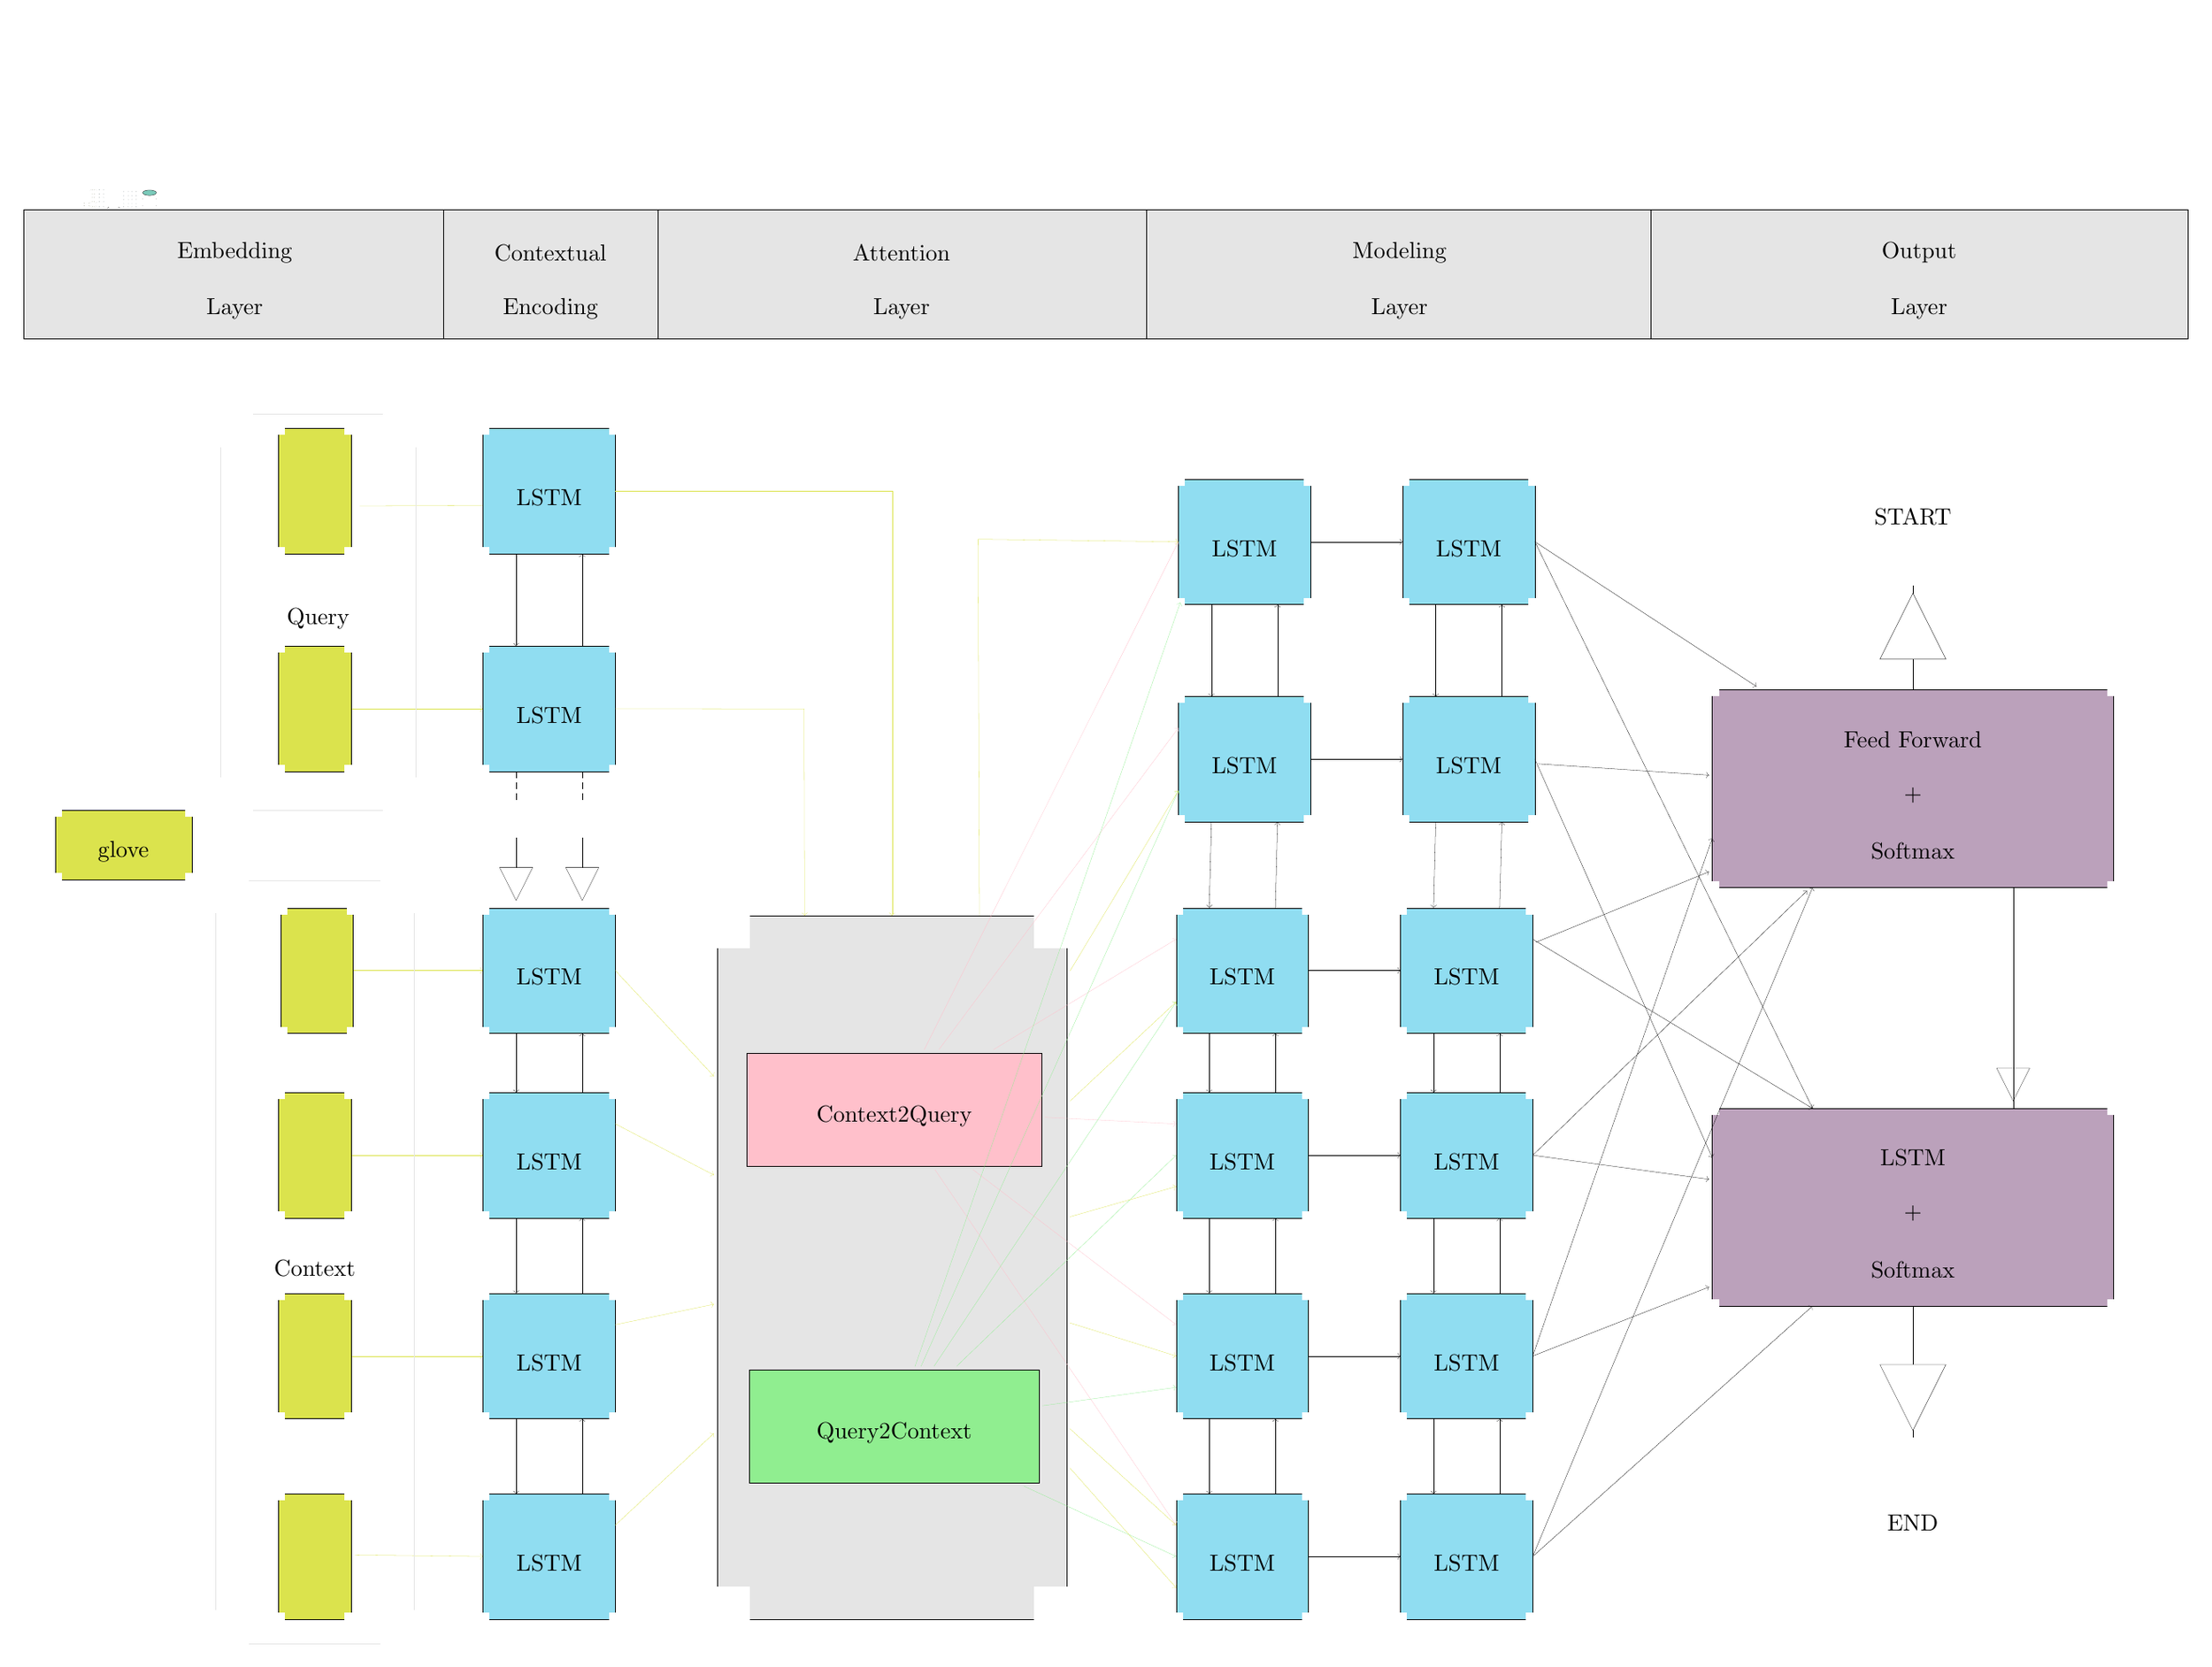
\begin{tikzpicture}
\pgftransformxscale{1.000000}
\pgftransformyscale{-1.000000}
\definecolor{dialinecolor}{rgb}{0.000000, 0.000000, 0.000000}
\pgfsetstrokecolor{dialinecolor}
\definecolor{dialinecolor}{rgb}{1.000000, 1.000000, 1.000000}
\pgfsetfillcolor{dialinecolor}
% setfont left to latex
\definecolor{dialinecolor}{rgb}{0.000000, 0.000000, 0.000000}
\pgfsetstrokecolor{dialinecolor}
\node at (3.142625\du,-2.277826\du){};
% setfont left to latex
\definecolor{dialinecolor}{rgb}{0.000000, 0.000000, 0.000000}
\pgfsetstrokecolor{dialinecolor}
\node at (7.008032\du,4.867120\du){};
% setfont left to latex
\definecolor{dialinecolor}{rgb}{0.000000, 0.000000, 0.000000}
\pgfsetstrokecolor{dialinecolor}
\node at (7.008032\du,4.867120\du){};
\pgfsetlinewidth{0.100000\du}
\pgfsetdash{}{0pt}
\pgfsetdash{}{0pt}
\pgfsetbuttcap
{
\definecolor{dialinecolor}{rgb}{0.858824, 0.890196, 0.301961}
\pgfsetfillcolor{dialinecolor}
% was here!!!
\pgfsetarrowsend{to}
\definecolor{dialinecolor}{rgb}{0.858824, 0.890196, 0.301961}
\pgfsetstrokecolor{dialinecolor}
\draw (4.161315\du,4.924215\du)--(6.127982\du,4.917537\du);
}
\pgfsetlinewidth{0.100000\du}
\pgfsetdash{}{0pt}
\pgfsetdash{}{0pt}
\pgfsetbuttcap
{
\definecolor{dialinecolor}{rgb}{0.858824, 0.890196, 0.301961}
\pgfsetfillcolor{dialinecolor}
% was here!!!
\pgfsetarrowsend{to}
\definecolor{dialinecolor}{rgb}{0.858824, 0.890196, 0.301961}
\pgfsetstrokecolor{dialinecolor}
\draw (4.028082\du,7.997537\du)--(6.029815\du,7.997537\du);
}
\pgfsetlinewidth{0.100000\du}
\pgfsetdash{}{0pt}
\pgfsetdash{}{0pt}
\pgfsetbuttcap
{
\definecolor{dialinecolor}{rgb}{0.858824, 0.890196, 0.301961}
\pgfsetfillcolor{dialinecolor}
% was here!!!
\pgfsetarrowsend{to}
\definecolor{dialinecolor}{rgb}{0.858824, 0.890196, 0.301961}
\pgfsetstrokecolor{dialinecolor}
\draw (4.061415\du,11.967537\du)--(6.029815\du,11.967537\du);
}
\pgfsetlinewidth{0.100000\du}
\pgfsetdash{}{0pt}
\pgfsetdash{}{0pt}
\pgfsetbuttcap
{
\definecolor{dialinecolor}{rgb}{0.858824, 0.890196, 0.301961}
\pgfsetfillcolor{dialinecolor}
% was here!!!
\pgfsetarrowsend{to}
\definecolor{dialinecolor}{rgb}{0.858824, 0.890196, 0.301961}
\pgfsetstrokecolor{dialinecolor}
\draw (4.028082\du,14.767537\du)--(6.029815\du,14.767537\du);
}
\pgfsetlinewidth{0.100000\du}
\pgfsetdash{}{0pt}
\pgfsetdash{}{0pt}
\pgfsetbuttcap
{
\definecolor{dialinecolor}{rgb}{0.858824, 0.890196, 0.301961}
\pgfsetfillcolor{dialinecolor}
% was here!!!
\pgfsetarrowsend{to}
\definecolor{dialinecolor}{rgb}{0.858824, 0.890196, 0.301961}
\pgfsetstrokecolor{dialinecolor}
\draw (4.028082\du,17.811757\du)--(6.029815\du,17.811757\du);
}
\pgfsetlinewidth{0.100000\du}
\pgfsetdash{}{0pt}
\pgfsetdash{}{0pt}
\pgfsetbuttcap
{
\definecolor{dialinecolor}{rgb}{0.858824, 0.890196, 0.301961}
\pgfsetfillcolor{dialinecolor}
% was here!!!
\pgfsetarrowsend{to}
\definecolor{dialinecolor}{rgb}{0.858824, 0.890196, 0.301961}
\pgfsetstrokecolor{dialinecolor}
\draw (4.088251\du,20.828682\du)--(6.029815\du,20.850870\du);
}
\pgfsetlinewidth{0.100000\du}
\pgfsetdash{}{0pt}
\pgfsetdash{}{0pt}
\pgfsetbuttcap
{
\definecolor{dialinecolor}{rgb}{0.000000, 0.000000, 0.000000}
\pgfsetfillcolor{dialinecolor}
% was here!!!
}
\definecolor{dialinecolor}{rgb}{0.000000, 0.000000, 0.000000}
\pgfsetstrokecolor{dialinecolor}
\draw (6.530857\du,9.947537\du)--(6.530857\du,10.405734\du);
\pgfsetlinewidth{0.100000\du}
\pgfsetdash{}{0pt}
\definecolor{dialinecolor}{rgb}{0.000000, 0.000000, 0.000000}
\pgfsetstrokecolor{dialinecolor}
\draw (6.530857\du,8.947537\du)--(6.530857\du,9.047537\du);
\definecolor{dialinecolor}{rgb}{0.000000, 0.000000, 0.000000}
\pgfsetstrokecolor{dialinecolor}
\draw (6.530857\du,9.114204\du)--(6.530857\du,9.214204\du);
\definecolor{dialinecolor}{rgb}{0.000000, 0.000000, 0.000000}
\pgfsetstrokecolor{dialinecolor}
\draw (6.530857\du,9.280870\du)--(6.530857\du,9.380870\du);
\pgfsetlinewidth{0.100000\du}
\pgfsetdash{}{0pt}
\pgfsetmiterjoin
\definecolor{dialinecolor}{rgb}{0.000000, 0.000000, 0.000000}
\pgfsetstrokecolor{dialinecolor}
\draw (6.280857\du,10.405734\du)--(6.530857\du,10.905734\du)--(6.780857\du,10.405734\du)--cycle;
\pgfsetlinewidth{0.100000\du}
\pgfsetdash{}{0pt}
\pgfsetdash{}{0pt}
\pgfsetmiterjoin
\definecolor{dialinecolor}{rgb}{0.898039, 0.898039, 0.898039}
\pgfsetstrokecolor{dialinecolor}
\draw (2.544748\du,3.534204\du)--(4.511415\du,3.534204\du);
\definecolor{dialinecolor}{rgb}{0.898039, 0.898039, 0.898039}
\pgfsetstrokecolor{dialinecolor}
\draw (2.544748\du,9.534204\du)--(4.511415\du,9.534204\du);
\definecolor{dialinecolor}{rgb}{0.898039, 0.898039, 0.898039}
\pgfsetstrokecolor{dialinecolor}
\pgfpathmoveto{\pgfpoint{2.544761\du}{3.534204\du}}
\pgfpatharc{270}{180}{0.500000\du and 0.500000\du}
\pgfusepath{stroke}
\definecolor{dialinecolor}{rgb}{0.898039, 0.898039, 0.898039}
\pgfsetstrokecolor{dialinecolor}
\pgfpathmoveto{\pgfpoint{5.011415\du}{4.034204\du}}
\pgfpatharc{360}{270}{0.500000\du and 0.500000\du}
\pgfusepath{stroke}
\definecolor{dialinecolor}{rgb}{0.898039, 0.898039, 0.898039}
\pgfsetstrokecolor{dialinecolor}
\draw (2.044748\du,4.034204\du)--(2.044748\du,9.034204\du);
\definecolor{dialinecolor}{rgb}{0.898039, 0.898039, 0.898039}
\pgfsetstrokecolor{dialinecolor}
\draw (5.011415\du,4.034204\du)--(5.011415\du,9.034204\du);
\definecolor{dialinecolor}{rgb}{0.898039, 0.898039, 0.898039}
\pgfsetstrokecolor{dialinecolor}
\pgfpathmoveto{\pgfpoint{2.044748\du}{9.034177\du}}
\pgfpatharc{180}{90}{0.500000\du and 0.500000\du}
\pgfusepath{stroke}
\definecolor{dialinecolor}{rgb}{0.898039, 0.898039, 0.898039}
\pgfsetstrokecolor{dialinecolor}
\pgfpathmoveto{\pgfpoint{4.511375\du}{9.534204\du}}
\pgfpatharc{90}{0}{0.500000\du and 0.500000\du}
\pgfusepath{stroke}
% setfont left to latex
\definecolor{dialinecolor}{rgb}{0.000000, 0.000000, 0.000000}
\pgfsetstrokecolor{dialinecolor}
\node at (3.528082\du,6.635037\du){Query};
\definecolor{dialinecolor}{rgb}{0.858824, 0.890196, 0.301961}
\pgfsetfillcolor{dialinecolor}
\fill (3.028082\du,7.047537\du)--(3.028082\du,8.947537\du)--(3.928082\du,8.947537\du)--(3.928082\du,7.047537\du)--cycle;
\definecolor{dialinecolor}{rgb}{0.858824, 0.890196, 0.301961}
\pgfsetfillcolor{dialinecolor}
\pgfpathmoveto{\pgfpoint{3.028084\du}{7.047537\du}}
\pgfpatharc{270}{180}{0.100000\du and 0.100000\du}
\pgfusepath{fill}
\definecolor{dialinecolor}{rgb}{0.858824, 0.890196, 0.301961}
\pgfsetfillcolor{dialinecolor}
\pgfpathmoveto{\pgfpoint{4.028082\du}{7.147537\du}}
\pgfpatharc{360}{270}{0.100000\du and 0.100000\du}
\pgfusepath{fill}
\definecolor{dialinecolor}{rgb}{0.858824, 0.890196, 0.301961}
\pgfsetfillcolor{dialinecolor}
\fill (2.928082\du,7.147537\du)--(2.928082\du,8.847537\du)--(4.028082\du,8.847537\du)--(4.028082\du,7.147537\du)--cycle;
\definecolor{dialinecolor}{rgb}{0.858824, 0.890196, 0.301961}
\pgfsetfillcolor{dialinecolor}
\pgfpathmoveto{\pgfpoint{2.928082\du}{8.847532\du}}
\pgfpatharc{180}{90}{0.100000\du and 0.100000\du}
\pgfusepath{fill}
\definecolor{dialinecolor}{rgb}{0.858824, 0.890196, 0.301961}
\pgfsetfillcolor{dialinecolor}
\pgfpathmoveto{\pgfpoint{3.928074\du}{8.947537\du}}
\pgfpatharc{90}{0}{0.100000\du and 0.100000\du}
\pgfusepath{fill}
\pgfsetlinewidth{0.100000\du}
\pgfsetdash{}{0pt}
\pgfsetdash{}{0pt}
\pgfsetmiterjoin
\definecolor{dialinecolor}{rgb}{0.000000, 0.000000, 0.000000}
\pgfsetstrokecolor{dialinecolor}
\draw (3.028082\du,7.047537\du)--(3.928082\du,7.047537\du);
\definecolor{dialinecolor}{rgb}{0.000000, 0.000000, 0.000000}
\pgfsetstrokecolor{dialinecolor}
\draw (3.028082\du,8.947537\du)--(3.928082\du,8.947537\du);
\definecolor{dialinecolor}{rgb}{0.000000, 0.000000, 0.000000}
\pgfsetstrokecolor{dialinecolor}
\pgfpathmoveto{\pgfpoint{3.028084\du}{7.047537\du}}
\pgfpatharc{270}{180}{0.100000\du and 0.100000\du}
\pgfusepath{stroke}
\definecolor{dialinecolor}{rgb}{0.000000, 0.000000, 0.000000}
\pgfsetstrokecolor{dialinecolor}
\pgfpathmoveto{\pgfpoint{4.028082\du}{7.147537\du}}
\pgfpatharc{360}{270}{0.100000\du and 0.100000\du}
\pgfusepath{stroke}
\definecolor{dialinecolor}{rgb}{0.000000, 0.000000, 0.000000}
\pgfsetstrokecolor{dialinecolor}
\draw (2.928082\du,7.147537\du)--(2.928082\du,8.847537\du);
\definecolor{dialinecolor}{rgb}{0.000000, 0.000000, 0.000000}
\pgfsetstrokecolor{dialinecolor}
\draw (4.028082\du,7.147537\du)--(4.028082\du,8.847537\du);
\definecolor{dialinecolor}{rgb}{0.000000, 0.000000, 0.000000}
\pgfsetstrokecolor{dialinecolor}
\pgfpathmoveto{\pgfpoint{2.928082\du}{8.847532\du}}
\pgfpatharc{180}{90}{0.100000\du and 0.100000\du}
\pgfusepath{stroke}
\definecolor{dialinecolor}{rgb}{0.000000, 0.000000, 0.000000}
\pgfsetstrokecolor{dialinecolor}
\pgfpathmoveto{\pgfpoint{3.928074\du}{8.947537\du}}
\pgfpatharc{90}{0}{0.100000\du and 0.100000\du}
\pgfusepath{stroke}
% setfont left to latex
\definecolor{dialinecolor}{rgb}{0.000000, 0.000000, 0.000000}
\pgfsetstrokecolor{dialinecolor}
\node at (3.478082\du,8.192537\du){};
\definecolor{dialinecolor}{rgb}{0.858824, 0.890196, 0.301961}
\pgfsetfillcolor{dialinecolor}
\fill (3.028082\du,3.750870\du)--(3.028082\du,5.650870\du)--(3.928082\du,5.650870\du)--(3.928082\du,3.750870\du)--cycle;
\definecolor{dialinecolor}{rgb}{0.858824, 0.890196, 0.301961}
\pgfsetfillcolor{dialinecolor}
\pgfpathmoveto{\pgfpoint{3.028084\du}{3.750870\du}}
\pgfpatharc{270}{180}{0.100000\du and 0.100000\du}
\pgfusepath{fill}
\definecolor{dialinecolor}{rgb}{0.858824, 0.890196, 0.301961}
\pgfsetfillcolor{dialinecolor}
\pgfpathmoveto{\pgfpoint{4.028082\du}{3.850870\du}}
\pgfpatharc{360}{270}{0.100000\du and 0.100000\du}
\pgfusepath{fill}
\definecolor{dialinecolor}{rgb}{0.858824, 0.890196, 0.301961}
\pgfsetfillcolor{dialinecolor}
\fill (2.928082\du,3.850870\du)--(2.928082\du,5.550870\du)--(4.028082\du,5.550870\du)--(4.028082\du,3.850870\du)--cycle;
\definecolor{dialinecolor}{rgb}{0.858824, 0.890196, 0.301961}
\pgfsetfillcolor{dialinecolor}
\pgfpathmoveto{\pgfpoint{2.928082\du}{5.550865\du}}
\pgfpatharc{180}{90}{0.100000\du and 0.100000\du}
\pgfusepath{fill}
\definecolor{dialinecolor}{rgb}{0.858824, 0.890196, 0.301961}
\pgfsetfillcolor{dialinecolor}
\pgfpathmoveto{\pgfpoint{3.928074\du}{5.650870\du}}
\pgfpatharc{90}{0}{0.100000\du and 0.100000\du}
\pgfusepath{fill}
\pgfsetlinewidth{0.100000\du}
\pgfsetdash{}{0pt}
\pgfsetdash{}{0pt}
\pgfsetmiterjoin
\definecolor{dialinecolor}{rgb}{0.000000, 0.000000, 0.000000}
\pgfsetstrokecolor{dialinecolor}
\draw (3.028082\du,3.750870\du)--(3.928082\du,3.750870\du);
\definecolor{dialinecolor}{rgb}{0.000000, 0.000000, 0.000000}
\pgfsetstrokecolor{dialinecolor}
\draw (3.028082\du,5.650870\du)--(3.928082\du,5.650870\du);
\definecolor{dialinecolor}{rgb}{0.000000, 0.000000, 0.000000}
\pgfsetstrokecolor{dialinecolor}
\pgfpathmoveto{\pgfpoint{3.028084\du}{3.750870\du}}
\pgfpatharc{270}{180}{0.100000\du and 0.100000\du}
\pgfusepath{stroke}
\definecolor{dialinecolor}{rgb}{0.000000, 0.000000, 0.000000}
\pgfsetstrokecolor{dialinecolor}
\pgfpathmoveto{\pgfpoint{4.028082\du}{3.850870\du}}
\pgfpatharc{360}{270}{0.100000\du and 0.100000\du}
\pgfusepath{stroke}
\definecolor{dialinecolor}{rgb}{0.000000, 0.000000, 0.000000}
\pgfsetstrokecolor{dialinecolor}
\draw (2.928082\du,3.850870\du)--(2.928082\du,5.550870\du);
\definecolor{dialinecolor}{rgb}{0.000000, 0.000000, 0.000000}
\pgfsetstrokecolor{dialinecolor}
\draw (4.028082\du,3.850870\du)--(4.028082\du,5.550870\du);
\definecolor{dialinecolor}{rgb}{0.000000, 0.000000, 0.000000}
\pgfsetstrokecolor{dialinecolor}
\pgfpathmoveto{\pgfpoint{2.928082\du}{5.550865\du}}
\pgfpatharc{180}{90}{0.100000\du and 0.100000\du}
\pgfusepath{stroke}
\definecolor{dialinecolor}{rgb}{0.000000, 0.000000, 0.000000}
\pgfsetstrokecolor{dialinecolor}
\pgfpathmoveto{\pgfpoint{3.928074\du}{5.650870\du}}
\pgfpatharc{90}{0}{0.100000\du and 0.100000\du}
\pgfusepath{stroke}
% setfont left to latex
\definecolor{dialinecolor}{rgb}{0.000000, 0.000000, 0.000000}
\pgfsetstrokecolor{dialinecolor}
\node at (3.478082\du,4.895870\du){};
\pgfsetlinewidth{0.100000\du}
\pgfsetdash{}{0pt}
\pgfsetdash{}{0pt}
\pgfsetbuttcap
{
\definecolor{dialinecolor}{rgb}{0.000000, 0.000000, 0.000000}
\pgfsetfillcolor{dialinecolor}
% was here!!!
}
\definecolor{dialinecolor}{rgb}{0.000000, 0.000000, 0.000000}
\pgfsetstrokecolor{dialinecolor}
\draw (7.532940\du,9.947537\du)--(7.532940\du,10.405734\du);
\pgfsetlinewidth{0.100000\du}
\pgfsetdash{}{0pt}
\definecolor{dialinecolor}{rgb}{0.000000, 0.000000, 0.000000}
\pgfsetstrokecolor{dialinecolor}
\draw (7.532940\du,8.947537\du)--(7.532940\du,9.047537\du);
\definecolor{dialinecolor}{rgb}{0.000000, 0.000000, 0.000000}
\pgfsetstrokecolor{dialinecolor}
\draw (7.532940\du,9.114204\du)--(7.532940\du,9.214204\du);
\definecolor{dialinecolor}{rgb}{0.000000, 0.000000, 0.000000}
\pgfsetstrokecolor{dialinecolor}
\draw (7.532940\du,9.280870\du)--(7.532940\du,9.380870\du);
\pgfsetlinewidth{0.100000\du}
\pgfsetdash{}{0pt}
\pgfsetmiterjoin
\definecolor{dialinecolor}{rgb}{0.000000, 0.000000, 0.000000}
\pgfsetstrokecolor{dialinecolor}
\draw (7.282940\du,10.405734\du)--(7.532940\du,10.905734\du)--(7.782940\du,10.405734\du)--cycle;
\definecolor{dialinecolor}{rgb}{0.898039, 0.898039, 0.898039}
\pgfsetfillcolor{dialinecolor}
\fill (10.078082\du,11.134204\du)--(10.078082\du,21.800870\du)--(14.378082\du,21.800870\du)--(14.378082\du,11.134204\du)--cycle;
\definecolor{dialinecolor}{rgb}{0.898039, 0.898039, 0.898039}
\pgfsetfillcolor{dialinecolor}
\pgfpathmoveto{\pgfpoint{10.078095\du}{11.134204\du}}
\pgfpatharc{270}{180}{0.500000\du and 0.500000\du}
\pgfusepath{fill}
\definecolor{dialinecolor}{rgb}{0.898039, 0.898039, 0.898039}
\pgfsetfillcolor{dialinecolor}
\pgfpathmoveto{\pgfpoint{14.878082\du}{11.634204\du}}
\pgfpatharc{360}{270}{0.500000\du and 0.500000\du}
\pgfusepath{fill}
\definecolor{dialinecolor}{rgb}{0.898039, 0.898039, 0.898039}
\pgfsetfillcolor{dialinecolor}
\fill (9.578082\du,11.634204\du)--(9.578082\du,21.300870\du)--(14.878082\du,21.300870\du)--(14.878082\du,11.634204\du)--cycle;
\definecolor{dialinecolor}{rgb}{0.898039, 0.898039, 0.898039}
\pgfsetfillcolor{dialinecolor}
\pgfpathmoveto{\pgfpoint{9.578082\du}{21.300844\du}}
\pgfpatharc{180}{90}{0.500000\du and 0.500000\du}
\pgfusepath{fill}
\definecolor{dialinecolor}{rgb}{0.898039, 0.898039, 0.898039}
\pgfsetfillcolor{dialinecolor}
\pgfpathmoveto{\pgfpoint{14.378042\du}{21.800870\du}}
\pgfpatharc{90}{0}{0.500000\du and 0.500000\du}
\pgfusepath{fill}
\pgfsetlinewidth{0.100000\du}
\pgfsetdash{}{0pt}
\pgfsetdash{}{0pt}
\pgfsetmiterjoin
\definecolor{dialinecolor}{rgb}{0.000000, 0.000000, 0.000000}
\pgfsetstrokecolor{dialinecolor}
\draw (10.078082\du,11.134204\du)--(14.378082\du,11.134204\du);
\definecolor{dialinecolor}{rgb}{0.000000, 0.000000, 0.000000}
\pgfsetstrokecolor{dialinecolor}
\draw (10.078082\du,21.800870\du)--(14.378082\du,21.800870\du);
\definecolor{dialinecolor}{rgb}{0.000000, 0.000000, 0.000000}
\pgfsetstrokecolor{dialinecolor}
\pgfpathmoveto{\pgfpoint{10.078095\du}{11.134204\du}}
\pgfpatharc{270}{180}{0.500000\du and 0.500000\du}
\pgfusepath{stroke}
\definecolor{dialinecolor}{rgb}{0.000000, 0.000000, 0.000000}
\pgfsetstrokecolor{dialinecolor}
\pgfpathmoveto{\pgfpoint{14.878082\du}{11.634204\du}}
\pgfpatharc{360}{270}{0.500000\du and 0.500000\du}
\pgfusepath{stroke}
\definecolor{dialinecolor}{rgb}{0.000000, 0.000000, 0.000000}
\pgfsetstrokecolor{dialinecolor}
\draw (9.578082\du,11.634204\du)--(9.578082\du,21.300870\du);
\definecolor{dialinecolor}{rgb}{0.000000, 0.000000, 0.000000}
\pgfsetstrokecolor{dialinecolor}
\draw (14.878082\du,11.634204\du)--(14.878082\du,21.300870\du);
\definecolor{dialinecolor}{rgb}{0.000000, 0.000000, 0.000000}
\pgfsetstrokecolor{dialinecolor}
\pgfpathmoveto{\pgfpoint{9.578082\du}{21.300844\du}}
\pgfpatharc{180}{90}{0.500000\du and 0.500000\du}
\pgfusepath{stroke}
\definecolor{dialinecolor}{rgb}{0.000000, 0.000000, 0.000000}
\pgfsetstrokecolor{dialinecolor}
\pgfpathmoveto{\pgfpoint{14.378042\du}{21.800870\du}}
\pgfpatharc{90}{0}{0.500000\du and 0.500000\du}
\pgfusepath{stroke}
% setfont left to latex
\definecolor{dialinecolor}{rgb}{0.000000, 0.000000, 0.000000}
\pgfsetstrokecolor{dialinecolor}
\node at (12.228082\du,16.568370\du){};
\definecolor{dialinecolor}{rgb}{1.000000, 0.752941, 0.796078}
\pgfsetfillcolor{dialinecolor}
\fill (10.028082\du,13.217537\du)--(10.028082\du,14.934204\du)--(14.494748\du,14.934204\du)--(14.494748\du,13.217537\du)--cycle;
\pgfsetlinewidth{0.100000\du}
\pgfsetdash{}{0pt}
\pgfsetdash{}{0pt}
\pgfsetmiterjoin
\definecolor{dialinecolor}{rgb}{0.000000, 0.000000, 0.000000}
\pgfsetstrokecolor{dialinecolor}
\draw (10.028082\du,13.217537\du)--(10.028082\du,14.934204\du)--(14.494748\du,14.934204\du)--(14.494748\du,13.217537\du)--cycle;
% setfont left to latex
\definecolor{dialinecolor}{rgb}{0.000000, 0.000000, 0.000000}
\pgfsetstrokecolor{dialinecolor}
\node at (12.261415\du,14.176704\du){Context2Query};
\definecolor{dialinecolor}{rgb}{0.564706, 0.933333, 0.564706}
\pgfsetfillcolor{dialinecolor}
\fill (10.061415\du,18.017537\du)--(10.061415\du,19.734204\du)--(14.461415\du,19.734204\du)--(14.461415\du,18.017537\du)--cycle;
\pgfsetlinewidth{0.100000\du}
\pgfsetdash{}{0pt}
\pgfsetdash{}{0pt}
\pgfsetmiterjoin
\definecolor{dialinecolor}{rgb}{0.000000, 0.000000, 0.000000}
\pgfsetstrokecolor{dialinecolor}
\draw (10.061415\du,18.017537\du)--(10.061415\du,19.734204\du)--(14.461415\du,19.734204\du)--(14.461415\du,18.017537\du)--cycle;
% setfont left to latex
\definecolor{dialinecolor}{rgb}{0.000000, 0.000000, 0.000000}
\pgfsetstrokecolor{dialinecolor}
\node at (12.261415\du,18.976704\du){Query2Context};
\definecolor{dialinecolor}{rgb}{0.858824, 0.890196, 0.301961}
\pgfsetfillcolor{dialinecolor}
\fill (-0.355252\du,9.534204\du)--(-0.355252\du,10.584204\du)--(1.511415\du,10.584204\du)--(1.511415\du,9.534204\du)--cycle;
\definecolor{dialinecolor}{rgb}{0.858824, 0.890196, 0.301961}
\pgfsetfillcolor{dialinecolor}
\pgfpathmoveto{\pgfpoint{-0.355249\du}{9.534204\du}}
\pgfpatharc{270}{180}{0.100000\du and 0.100000\du}
\pgfusepath{fill}
\definecolor{dialinecolor}{rgb}{0.858824, 0.890196, 0.301961}
\pgfsetfillcolor{dialinecolor}
\pgfpathmoveto{\pgfpoint{1.611415\du}{9.634204\du}}
\pgfpatharc{360}{270}{0.100000\du and 0.100000\du}
\pgfusepath{fill}
\definecolor{dialinecolor}{rgb}{0.858824, 0.890196, 0.301961}
\pgfsetfillcolor{dialinecolor}
\fill (-0.455252\du,9.634204\du)--(-0.455252\du,10.484204\du)--(1.611415\du,10.484204\du)--(1.611415\du,9.634204\du)--cycle;
\definecolor{dialinecolor}{rgb}{0.858824, 0.890196, 0.301961}
\pgfsetfillcolor{dialinecolor}
\pgfpathmoveto{\pgfpoint{-0.455252\du}{10.484198\du}}
\pgfpatharc{180}{90}{0.100000\du and 0.100000\du}
\pgfusepath{fill}
\definecolor{dialinecolor}{rgb}{0.858824, 0.890196, 0.301961}
\pgfsetfillcolor{dialinecolor}
\pgfpathmoveto{\pgfpoint{1.511407\du}{10.584204\du}}
\pgfpatharc{90}{0}{0.100000\du and 0.100000\du}
\pgfusepath{fill}
\pgfsetlinewidth{0.100000\du}
\pgfsetdash{}{0pt}
\pgfsetdash{}{0pt}
\pgfsetmiterjoin
\definecolor{dialinecolor}{rgb}{0.000000, 0.000000, 0.000000}
\pgfsetstrokecolor{dialinecolor}
\draw (-0.355252\du,9.534204\du)--(1.511415\du,9.534204\du);
\definecolor{dialinecolor}{rgb}{0.000000, 0.000000, 0.000000}
\pgfsetstrokecolor{dialinecolor}
\draw (-0.355252\du,10.584204\du)--(1.511415\du,10.584204\du);
\definecolor{dialinecolor}{rgb}{0.000000, 0.000000, 0.000000}
\pgfsetstrokecolor{dialinecolor}
\pgfpathmoveto{\pgfpoint{-0.355249\du}{9.534204\du}}
\pgfpatharc{270}{180}{0.100000\du and 0.100000\du}
\pgfusepath{stroke}
\definecolor{dialinecolor}{rgb}{0.000000, 0.000000, 0.000000}
\pgfsetstrokecolor{dialinecolor}
\pgfpathmoveto{\pgfpoint{1.611415\du}{9.634204\du}}
\pgfpatharc{360}{270}{0.100000\du and 0.100000\du}
\pgfusepath{stroke}
\definecolor{dialinecolor}{rgb}{0.000000, 0.000000, 0.000000}
\pgfsetstrokecolor{dialinecolor}
\draw (-0.455252\du,9.634204\du)--(-0.455252\du,10.484204\du);
\definecolor{dialinecolor}{rgb}{0.000000, 0.000000, 0.000000}
\pgfsetstrokecolor{dialinecolor}
\draw (1.611415\du,9.634204\du)--(1.611415\du,10.484204\du);
\definecolor{dialinecolor}{rgb}{0.000000, 0.000000, 0.000000}
\pgfsetstrokecolor{dialinecolor}
\pgfpathmoveto{\pgfpoint{-0.455252\du}{10.484198\du}}
\pgfpatharc{180}{90}{0.100000\du and 0.100000\du}
\pgfusepath{stroke}
\definecolor{dialinecolor}{rgb}{0.000000, 0.000000, 0.000000}
\pgfsetstrokecolor{dialinecolor}
\pgfpathmoveto{\pgfpoint{1.511407\du}{10.584204\du}}
\pgfpatharc{90}{0}{0.100000\du and 0.100000\du}
\pgfusepath{stroke}
% setfont left to latex
\definecolor{dialinecolor}{rgb}{0.000000, 0.000000, 0.000000}
\pgfsetstrokecolor{dialinecolor}
\node at (0.578082\du,10.160037\du){glove};
\pgfsetlinewidth{0.100000\du}
\pgfsetdash{}{0pt}
\pgfsetdash{}{0pt}
\pgfsetmiterjoin
\definecolor{dialinecolor}{rgb}{0.898039, 0.898039, 0.898039}
\pgfsetstrokecolor{dialinecolor}
\draw (2.478082\du,10.600870\du)--(4.478082\du,10.600870\du);
\definecolor{dialinecolor}{rgb}{0.898039, 0.898039, 0.898039}
\pgfsetstrokecolor{dialinecolor}
\draw (2.478082\du,22.167537\du)--(4.478082\du,22.167537\du);
\definecolor{dialinecolor}{rgb}{0.898039, 0.898039, 0.898039}
\pgfsetstrokecolor{dialinecolor}
\pgfpathmoveto{\pgfpoint{2.478095\du}{10.600870\du}}
\pgfpatharc{270}{180}{0.500000\du and 0.500000\du}
\pgfusepath{stroke}
\definecolor{dialinecolor}{rgb}{0.898039, 0.898039, 0.898039}
\pgfsetstrokecolor{dialinecolor}
\pgfpathmoveto{\pgfpoint{4.978082\du}{11.100870\du}}
\pgfpatharc{360}{270}{0.500000\du and 0.500000\du}
\pgfusepath{stroke}
\definecolor{dialinecolor}{rgb}{0.898039, 0.898039, 0.898039}
\pgfsetstrokecolor{dialinecolor}
\draw (1.978082\du,11.100870\du)--(1.978082\du,21.667537\du);
\definecolor{dialinecolor}{rgb}{0.898039, 0.898039, 0.898039}
\pgfsetstrokecolor{dialinecolor}
\draw (4.978082\du,11.100870\du)--(4.978082\du,21.667537\du);
\definecolor{dialinecolor}{rgb}{0.898039, 0.898039, 0.898039}
\pgfsetstrokecolor{dialinecolor}
\pgfpathmoveto{\pgfpoint{1.978082\du}{21.667511\du}}
\pgfpatharc{180}{90}{0.500000\du and 0.500000\du}
\pgfusepath{stroke}
\definecolor{dialinecolor}{rgb}{0.898039, 0.898039, 0.898039}
\pgfsetstrokecolor{dialinecolor}
\pgfpathmoveto{\pgfpoint{4.478042\du}{22.167537\du}}
\pgfpatharc{90}{0}{0.500000\du and 0.500000\du}
\pgfusepath{stroke}
% setfont left to latex
\definecolor{dialinecolor}{rgb}{0.000000, 0.000000, 0.000000}
\pgfsetstrokecolor{dialinecolor}
\node at (3.478082\du,16.485037\du){Context};
\definecolor{dialinecolor}{rgb}{0.858824, 0.890196, 0.301961}
\pgfsetfillcolor{dialinecolor}
\fill (3.028082\du,16.861757\du)--(3.028082\du,18.761757\du)--(3.928082\du,18.761757\du)--(3.928082\du,16.861757\du)--cycle;
\definecolor{dialinecolor}{rgb}{0.858824, 0.890196, 0.301961}
\pgfsetfillcolor{dialinecolor}
\pgfpathmoveto{\pgfpoint{3.028084\du}{16.861757\du}}
\pgfpatharc{270}{180}{0.100000\du and 0.100000\du}
\pgfusepath{fill}
\definecolor{dialinecolor}{rgb}{0.858824, 0.890196, 0.301961}
\pgfsetfillcolor{dialinecolor}
\pgfpathmoveto{\pgfpoint{4.028082\du}{16.961757\du}}
\pgfpatharc{360}{270}{0.100000\du and 0.100000\du}
\pgfusepath{fill}
\definecolor{dialinecolor}{rgb}{0.858824, 0.890196, 0.301961}
\pgfsetfillcolor{dialinecolor}
\fill (2.928082\du,16.961757\du)--(2.928082\du,18.661757\du)--(4.028082\du,18.661757\du)--(4.028082\du,16.961757\du)--cycle;
\definecolor{dialinecolor}{rgb}{0.858824, 0.890196, 0.301961}
\pgfsetfillcolor{dialinecolor}
\pgfpathmoveto{\pgfpoint{2.928082\du}{18.661751\du}}
\pgfpatharc{180}{90}{0.100000\du and 0.100000\du}
\pgfusepath{fill}
\definecolor{dialinecolor}{rgb}{0.858824, 0.890196, 0.301961}
\pgfsetfillcolor{dialinecolor}
\pgfpathmoveto{\pgfpoint{3.928074\du}{18.761757\du}}
\pgfpatharc{90}{0}{0.100000\du and 0.100000\du}
\pgfusepath{fill}
\pgfsetlinewidth{0.100000\du}
\pgfsetdash{}{0pt}
\pgfsetdash{}{0pt}
\pgfsetmiterjoin
\definecolor{dialinecolor}{rgb}{0.000000, 0.000000, 0.000000}
\pgfsetstrokecolor{dialinecolor}
\draw (3.028082\du,16.861757\du)--(3.928082\du,16.861757\du);
\definecolor{dialinecolor}{rgb}{0.000000, 0.000000, 0.000000}
\pgfsetstrokecolor{dialinecolor}
\draw (3.028082\du,18.761757\du)--(3.928082\du,18.761757\du);
\definecolor{dialinecolor}{rgb}{0.000000, 0.000000, 0.000000}
\pgfsetstrokecolor{dialinecolor}
\pgfpathmoveto{\pgfpoint{3.028084\du}{16.861757\du}}
\pgfpatharc{270}{180}{0.100000\du and 0.100000\du}
\pgfusepath{stroke}
\definecolor{dialinecolor}{rgb}{0.000000, 0.000000, 0.000000}
\pgfsetstrokecolor{dialinecolor}
\pgfpathmoveto{\pgfpoint{4.028082\du}{16.961757\du}}
\pgfpatharc{360}{270}{0.100000\du and 0.100000\du}
\pgfusepath{stroke}
\definecolor{dialinecolor}{rgb}{0.000000, 0.000000, 0.000000}
\pgfsetstrokecolor{dialinecolor}
\draw (2.928082\du,16.961757\du)--(2.928082\du,18.661757\du);
\definecolor{dialinecolor}{rgb}{0.000000, 0.000000, 0.000000}
\pgfsetstrokecolor{dialinecolor}
\draw (4.028082\du,16.961757\du)--(4.028082\du,18.661757\du);
\definecolor{dialinecolor}{rgb}{0.000000, 0.000000, 0.000000}
\pgfsetstrokecolor{dialinecolor}
\pgfpathmoveto{\pgfpoint{2.928082\du}{18.661751\du}}
\pgfpatharc{180}{90}{0.100000\du and 0.100000\du}
\pgfusepath{stroke}
\definecolor{dialinecolor}{rgb}{0.000000, 0.000000, 0.000000}
\pgfsetstrokecolor{dialinecolor}
\pgfpathmoveto{\pgfpoint{3.928074\du}{18.761757\du}}
\pgfpatharc{90}{0}{0.100000\du and 0.100000\du}
\pgfusepath{stroke}
% setfont left to latex
\definecolor{dialinecolor}{rgb}{0.000000, 0.000000, 0.000000}
\pgfsetstrokecolor{dialinecolor}
\node at (3.478082\du,18.006757\du){};
\definecolor{dialinecolor}{rgb}{0.858824, 0.890196, 0.301961}
\pgfsetfillcolor{dialinecolor}
\fill (3.028082\du,13.817537\du)--(3.028082\du,15.717537\du)--(3.928082\du,15.717537\du)--(3.928082\du,13.817537\du)--cycle;
\definecolor{dialinecolor}{rgb}{0.858824, 0.890196, 0.301961}
\pgfsetfillcolor{dialinecolor}
\pgfpathmoveto{\pgfpoint{3.028084\du}{13.817537\du}}
\pgfpatharc{270}{180}{0.100000\du and 0.100000\du}
\pgfusepath{fill}
\definecolor{dialinecolor}{rgb}{0.858824, 0.890196, 0.301961}
\pgfsetfillcolor{dialinecolor}
\pgfpathmoveto{\pgfpoint{4.028082\du}{13.917537\du}}
\pgfpatharc{360}{270}{0.100000\du and 0.100000\du}
\pgfusepath{fill}
\definecolor{dialinecolor}{rgb}{0.858824, 0.890196, 0.301961}
\pgfsetfillcolor{dialinecolor}
\fill (2.928082\du,13.917537\du)--(2.928082\du,15.617537\du)--(4.028082\du,15.617537\du)--(4.028082\du,13.917537\du)--cycle;
\definecolor{dialinecolor}{rgb}{0.858824, 0.890196, 0.301961}
\pgfsetfillcolor{dialinecolor}
\pgfpathmoveto{\pgfpoint{2.928082\du}{15.617532\du}}
\pgfpatharc{180}{90}{0.100000\du and 0.100000\du}
\pgfusepath{fill}
\definecolor{dialinecolor}{rgb}{0.858824, 0.890196, 0.301961}
\pgfsetfillcolor{dialinecolor}
\pgfpathmoveto{\pgfpoint{3.928074\du}{15.717537\du}}
\pgfpatharc{90}{0}{0.100000\du and 0.100000\du}
\pgfusepath{fill}
\pgfsetlinewidth{0.100000\du}
\pgfsetdash{}{0pt}
\pgfsetdash{}{0pt}
\pgfsetmiterjoin
\definecolor{dialinecolor}{rgb}{0.000000, 0.000000, 0.000000}
\pgfsetstrokecolor{dialinecolor}
\draw (3.028082\du,13.817537\du)--(3.928082\du,13.817537\du);
\definecolor{dialinecolor}{rgb}{0.000000, 0.000000, 0.000000}
\pgfsetstrokecolor{dialinecolor}
\draw (3.028082\du,15.717537\du)--(3.928082\du,15.717537\du);
\definecolor{dialinecolor}{rgb}{0.000000, 0.000000, 0.000000}
\pgfsetstrokecolor{dialinecolor}
\pgfpathmoveto{\pgfpoint{3.028084\du}{13.817537\du}}
\pgfpatharc{270}{180}{0.100000\du and 0.100000\du}
\pgfusepath{stroke}
\definecolor{dialinecolor}{rgb}{0.000000, 0.000000, 0.000000}
\pgfsetstrokecolor{dialinecolor}
\pgfpathmoveto{\pgfpoint{4.028082\du}{13.917537\du}}
\pgfpatharc{360}{270}{0.100000\du and 0.100000\du}
\pgfusepath{stroke}
\definecolor{dialinecolor}{rgb}{0.000000, 0.000000, 0.000000}
\pgfsetstrokecolor{dialinecolor}
\draw (2.928082\du,13.917537\du)--(2.928082\du,15.617537\du);
\definecolor{dialinecolor}{rgb}{0.000000, 0.000000, 0.000000}
\pgfsetstrokecolor{dialinecolor}
\draw (4.028082\du,13.917537\du)--(4.028082\du,15.617537\du);
\definecolor{dialinecolor}{rgb}{0.000000, 0.000000, 0.000000}
\pgfsetstrokecolor{dialinecolor}
\pgfpathmoveto{\pgfpoint{2.928082\du}{15.617532\du}}
\pgfpatharc{180}{90}{0.100000\du and 0.100000\du}
\pgfusepath{stroke}
\definecolor{dialinecolor}{rgb}{0.000000, 0.000000, 0.000000}
\pgfsetstrokecolor{dialinecolor}
\pgfpathmoveto{\pgfpoint{3.928074\du}{15.717537\du}}
\pgfpatharc{90}{0}{0.100000\du and 0.100000\du}
\pgfusepath{stroke}
% setfont left to latex
\definecolor{dialinecolor}{rgb}{0.000000, 0.000000, 0.000000}
\pgfsetstrokecolor{dialinecolor}
\node at (3.478082\du,14.962537\du){};
\definecolor{dialinecolor}{rgb}{0.858824, 0.890196, 0.301961}
\pgfsetfillcolor{dialinecolor}
\fill (3.061415\du,11.017537\du)--(3.061415\du,12.917537\du)--(3.961415\du,12.917537\du)--(3.961415\du,11.017537\du)--cycle;
\definecolor{dialinecolor}{rgb}{0.858824, 0.890196, 0.301961}
\pgfsetfillcolor{dialinecolor}
\pgfpathmoveto{\pgfpoint{3.061418\du}{11.017537\du}}
\pgfpatharc{270}{180}{0.100000\du and 0.100000\du}
\pgfusepath{fill}
\definecolor{dialinecolor}{rgb}{0.858824, 0.890196, 0.301961}
\pgfsetfillcolor{dialinecolor}
\pgfpathmoveto{\pgfpoint{4.061415\du}{11.117537\du}}
\pgfpatharc{360}{270}{0.100000\du and 0.100000\du}
\pgfusepath{fill}
\definecolor{dialinecolor}{rgb}{0.858824, 0.890196, 0.301961}
\pgfsetfillcolor{dialinecolor}
\fill (2.961415\du,11.117537\du)--(2.961415\du,12.817537\du)--(4.061415\du,12.817537\du)--(4.061415\du,11.117537\du)--cycle;
\definecolor{dialinecolor}{rgb}{0.858824, 0.890196, 0.301961}
\pgfsetfillcolor{dialinecolor}
\pgfpathmoveto{\pgfpoint{2.961415\du}{12.817532\du}}
\pgfpatharc{180}{90}{0.100000\du and 0.100000\du}
\pgfusepath{fill}
\definecolor{dialinecolor}{rgb}{0.858824, 0.890196, 0.301961}
\pgfsetfillcolor{dialinecolor}
\pgfpathmoveto{\pgfpoint{3.961407\du}{12.917537\du}}
\pgfpatharc{90}{0}{0.100000\du and 0.100000\du}
\pgfusepath{fill}
\pgfsetlinewidth{0.100000\du}
\pgfsetdash{}{0pt}
\pgfsetdash{}{0pt}
\pgfsetmiterjoin
\definecolor{dialinecolor}{rgb}{0.000000, 0.000000, 0.000000}
\pgfsetstrokecolor{dialinecolor}
\draw (3.061415\du,11.017537\du)--(3.961415\du,11.017537\du);
\definecolor{dialinecolor}{rgb}{0.000000, 0.000000, 0.000000}
\pgfsetstrokecolor{dialinecolor}
\draw (3.061415\du,12.917537\du)--(3.961415\du,12.917537\du);
\definecolor{dialinecolor}{rgb}{0.000000, 0.000000, 0.000000}
\pgfsetstrokecolor{dialinecolor}
\pgfpathmoveto{\pgfpoint{3.061418\du}{11.017537\du}}
\pgfpatharc{270}{180}{0.100000\du and 0.100000\du}
\pgfusepath{stroke}
\definecolor{dialinecolor}{rgb}{0.000000, 0.000000, 0.000000}
\pgfsetstrokecolor{dialinecolor}
\pgfpathmoveto{\pgfpoint{4.061415\du}{11.117537\du}}
\pgfpatharc{360}{270}{0.100000\du and 0.100000\du}
\pgfusepath{stroke}
\definecolor{dialinecolor}{rgb}{0.000000, 0.000000, 0.000000}
\pgfsetstrokecolor{dialinecolor}
\draw (2.961415\du,11.117537\du)--(2.961415\du,12.817537\du);
\definecolor{dialinecolor}{rgb}{0.000000, 0.000000, 0.000000}
\pgfsetstrokecolor{dialinecolor}
\draw (4.061415\du,11.117537\du)--(4.061415\du,12.817537\du);
\definecolor{dialinecolor}{rgb}{0.000000, 0.000000, 0.000000}
\pgfsetstrokecolor{dialinecolor}
\pgfpathmoveto{\pgfpoint{2.961415\du}{12.817532\du}}
\pgfpatharc{180}{90}{0.100000\du and 0.100000\du}
\pgfusepath{stroke}
\definecolor{dialinecolor}{rgb}{0.000000, 0.000000, 0.000000}
\pgfsetstrokecolor{dialinecolor}
\pgfpathmoveto{\pgfpoint{3.961407\du}{12.917537\du}}
\pgfpatharc{90}{0}{0.100000\du and 0.100000\du}
\pgfusepath{stroke}
% setfont left to latex
\definecolor{dialinecolor}{rgb}{0.000000, 0.000000, 0.000000}
\pgfsetstrokecolor{dialinecolor}
\node at (3.511415\du,12.162537\du){};
\definecolor{dialinecolor}{rgb}{0.858824, 0.890196, 0.301961}
\pgfsetfillcolor{dialinecolor}
\fill (3.028082\du,19.900870\du)--(3.028082\du,21.800870\du)--(3.928082\du,21.800870\du)--(3.928082\du,19.900870\du)--cycle;
\definecolor{dialinecolor}{rgb}{0.858824, 0.890196, 0.301961}
\pgfsetfillcolor{dialinecolor}
\pgfpathmoveto{\pgfpoint{3.028084\du}{19.900870\du}}
\pgfpatharc{270}{180}{0.100000\du and 0.100000\du}
\pgfusepath{fill}
\definecolor{dialinecolor}{rgb}{0.858824, 0.890196, 0.301961}
\pgfsetfillcolor{dialinecolor}
\pgfpathmoveto{\pgfpoint{4.028082\du}{20.000870\du}}
\pgfpatharc{360}{270}{0.100000\du and 0.100000\du}
\pgfusepath{fill}
\definecolor{dialinecolor}{rgb}{0.858824, 0.890196, 0.301961}
\pgfsetfillcolor{dialinecolor}
\fill (2.928082\du,20.000870\du)--(2.928082\du,21.700870\du)--(4.028082\du,21.700870\du)--(4.028082\du,20.000870\du)--cycle;
\definecolor{dialinecolor}{rgb}{0.858824, 0.890196, 0.301961}
\pgfsetfillcolor{dialinecolor}
\pgfpathmoveto{\pgfpoint{2.928082\du}{21.700865\du}}
\pgfpatharc{180}{90}{0.100000\du and 0.100000\du}
\pgfusepath{fill}
\definecolor{dialinecolor}{rgb}{0.858824, 0.890196, 0.301961}
\pgfsetfillcolor{dialinecolor}
\pgfpathmoveto{\pgfpoint{3.928074\du}{21.800870\du}}
\pgfpatharc{90}{0}{0.100000\du and 0.100000\du}
\pgfusepath{fill}
\pgfsetlinewidth{0.100000\du}
\pgfsetdash{}{0pt}
\pgfsetdash{}{0pt}
\pgfsetmiterjoin
\definecolor{dialinecolor}{rgb}{0.000000, 0.000000, 0.000000}
\pgfsetstrokecolor{dialinecolor}
\draw (3.028082\du,19.900870\du)--(3.928082\du,19.900870\du);
\definecolor{dialinecolor}{rgb}{0.000000, 0.000000, 0.000000}
\pgfsetstrokecolor{dialinecolor}
\draw (3.028082\du,21.800870\du)--(3.928082\du,21.800870\du);
\definecolor{dialinecolor}{rgb}{0.000000, 0.000000, 0.000000}
\pgfsetstrokecolor{dialinecolor}
\pgfpathmoveto{\pgfpoint{3.028084\du}{19.900870\du}}
\pgfpatharc{270}{180}{0.100000\du and 0.100000\du}
\pgfusepath{stroke}
\definecolor{dialinecolor}{rgb}{0.000000, 0.000000, 0.000000}
\pgfsetstrokecolor{dialinecolor}
\pgfpathmoveto{\pgfpoint{4.028082\du}{20.000870\du}}
\pgfpatharc{360}{270}{0.100000\du and 0.100000\du}
\pgfusepath{stroke}
\definecolor{dialinecolor}{rgb}{0.000000, 0.000000, 0.000000}
\pgfsetstrokecolor{dialinecolor}
\draw (2.928082\du,20.000870\du)--(2.928082\du,21.700870\du);
\definecolor{dialinecolor}{rgb}{0.000000, 0.000000, 0.000000}
\pgfsetstrokecolor{dialinecolor}
\draw (4.028082\du,20.000870\du)--(4.028082\du,21.700870\du);
\definecolor{dialinecolor}{rgb}{0.000000, 0.000000, 0.000000}
\pgfsetstrokecolor{dialinecolor}
\pgfpathmoveto{\pgfpoint{2.928082\du}{21.700865\du}}
\pgfpatharc{180}{90}{0.100000\du and 0.100000\du}
\pgfusepath{stroke}
\definecolor{dialinecolor}{rgb}{0.000000, 0.000000, 0.000000}
\pgfsetstrokecolor{dialinecolor}
\pgfpathmoveto{\pgfpoint{3.928074\du}{21.800870\du}}
\pgfpatharc{90}{0}{0.100000\du and 0.100000\du}
\pgfusepath{stroke}
% setfont left to latex
\definecolor{dialinecolor}{rgb}{0.000000, 0.000000, 0.000000}
\pgfsetstrokecolor{dialinecolor}
\node at (3.478082\du,21.045870\du){};
\definecolor{dialinecolor}{rgb}{0.564706, 0.866667, 0.945098}
\pgfsetfillcolor{dialinecolor}
\fill (6.129815\du,7.047537\du)--(6.129815\du,8.947537\du)--(7.933982\du,8.947537\du)--(7.933982\du,7.047537\du)--cycle;
\definecolor{dialinecolor}{rgb}{0.564706, 0.866667, 0.945098}
\pgfsetfillcolor{dialinecolor}
\pgfpathmoveto{\pgfpoint{6.129818\du}{7.047537\du}}
\pgfpatharc{270}{180}{0.100000\du and 0.100000\du}
\pgfusepath{fill}
\definecolor{dialinecolor}{rgb}{0.564706, 0.866667, 0.945098}
\pgfsetfillcolor{dialinecolor}
\pgfpathmoveto{\pgfpoint{8.033982\du}{7.147537\du}}
\pgfpatharc{360}{270}{0.100000\du and 0.100000\du}
\pgfusepath{fill}
\definecolor{dialinecolor}{rgb}{0.564706, 0.866667, 0.945098}
\pgfsetfillcolor{dialinecolor}
\fill (6.029815\du,7.147537\du)--(6.029815\du,8.847537\du)--(8.033982\du,8.847537\du)--(8.033982\du,7.147537\du)--cycle;
\definecolor{dialinecolor}{rgb}{0.564706, 0.866667, 0.945098}
\pgfsetfillcolor{dialinecolor}
\pgfpathmoveto{\pgfpoint{6.029815\du}{8.847532\du}}
\pgfpatharc{180}{90}{0.100000\du and 0.100000\du}
\pgfusepath{fill}
\definecolor{dialinecolor}{rgb}{0.564706, 0.866667, 0.945098}
\pgfsetfillcolor{dialinecolor}
\pgfpathmoveto{\pgfpoint{7.933974\du}{8.947537\du}}
\pgfpatharc{90}{0}{0.100000\du and 0.100000\du}
\pgfusepath{fill}
\pgfsetlinewidth{0.100000\du}
\pgfsetdash{}{0pt}
\pgfsetdash{}{0pt}
\pgfsetmiterjoin
\definecolor{dialinecolor}{rgb}{0.000000, 0.000000, 0.000000}
\pgfsetstrokecolor{dialinecolor}
\draw (6.129815\du,7.047537\du)--(7.933982\du,7.047537\du);
\definecolor{dialinecolor}{rgb}{0.000000, 0.000000, 0.000000}
\pgfsetstrokecolor{dialinecolor}
\draw (6.129815\du,8.947537\du)--(7.933982\du,8.947537\du);
\definecolor{dialinecolor}{rgb}{0.000000, 0.000000, 0.000000}
\pgfsetstrokecolor{dialinecolor}
\pgfpathmoveto{\pgfpoint{6.129818\du}{7.047537\du}}
\pgfpatharc{270}{180}{0.100000\du and 0.100000\du}
\pgfusepath{stroke}
\definecolor{dialinecolor}{rgb}{0.000000, 0.000000, 0.000000}
\pgfsetstrokecolor{dialinecolor}
\pgfpathmoveto{\pgfpoint{8.033982\du}{7.147537\du}}
\pgfpatharc{360}{270}{0.100000\du and 0.100000\du}
\pgfusepath{stroke}
\definecolor{dialinecolor}{rgb}{0.000000, 0.000000, 0.000000}
\pgfsetstrokecolor{dialinecolor}
\draw (6.029815\du,7.147537\du)--(6.029815\du,8.847537\du);
\definecolor{dialinecolor}{rgb}{0.000000, 0.000000, 0.000000}
\pgfsetstrokecolor{dialinecolor}
\draw (8.033982\du,7.147537\du)--(8.033982\du,8.847537\du);
\definecolor{dialinecolor}{rgb}{0.000000, 0.000000, 0.000000}
\pgfsetstrokecolor{dialinecolor}
\pgfpathmoveto{\pgfpoint{6.029815\du}{8.847532\du}}
\pgfpatharc{180}{90}{0.100000\du and 0.100000\du}
\pgfusepath{stroke}
\definecolor{dialinecolor}{rgb}{0.000000, 0.000000, 0.000000}
\pgfsetstrokecolor{dialinecolor}
\pgfpathmoveto{\pgfpoint{7.933974\du}{8.947537\du}}
\pgfpatharc{90}{0}{0.100000\du and 0.100000\du}
\pgfusepath{stroke}
% setfont left to latex
\definecolor{dialinecolor}{rgb}{0.000000, 0.000000, 0.000000}
\pgfsetstrokecolor{dialinecolor}
\node at (7.031898\du,8.098370\du){LSTM};
\pgfsetlinewidth{0.100000\du}
\pgfsetdash{}{0pt}
\pgfsetdash{}{0pt}
\pgfsetbuttcap
{
\definecolor{dialinecolor}{rgb}{0.000000, 0.000000, 0.000000}
\pgfsetfillcolor{dialinecolor}
% was here!!!
\pgfsetarrowsend{to}
\definecolor{dialinecolor}{rgb}{0.000000, 0.000000, 0.000000}
\pgfsetstrokecolor{dialinecolor}
\draw (6.530857\du,5.650870\du)--(6.530857\du,7.047537\du);
}
\pgfsetlinewidth{0.100000\du}
\pgfsetdash{}{0pt}
\pgfsetdash{}{0pt}
\pgfsetbuttcap
{
\definecolor{dialinecolor}{rgb}{0.000000, 0.000000, 0.000000}
\pgfsetfillcolor{dialinecolor}
% was here!!!
\pgfsetarrowsend{to}
\definecolor{dialinecolor}{rgb}{0.000000, 0.000000, 0.000000}
\pgfsetstrokecolor{dialinecolor}
\draw (7.532940\du,7.047537\du)--(7.532940\du,5.650870\du);
}
\definecolor{dialinecolor}{rgb}{0.564706, 0.866667, 0.945098}
\pgfsetfillcolor{dialinecolor}
\fill (6.129815\du,3.750870\du)--(6.129815\du,5.650870\du)--(7.933982\du,5.650870\du)--(7.933982\du,3.750870\du)--cycle;
\definecolor{dialinecolor}{rgb}{0.564706, 0.866667, 0.945098}
\pgfsetfillcolor{dialinecolor}
\pgfpathmoveto{\pgfpoint{6.129818\du}{3.750870\du}}
\pgfpatharc{270}{180}{0.100000\du and 0.100000\du}
\pgfusepath{fill}
\definecolor{dialinecolor}{rgb}{0.564706, 0.866667, 0.945098}
\pgfsetfillcolor{dialinecolor}
\pgfpathmoveto{\pgfpoint{8.033982\du}{3.850870\du}}
\pgfpatharc{360}{270}{0.100000\du and 0.100000\du}
\pgfusepath{fill}
\definecolor{dialinecolor}{rgb}{0.564706, 0.866667, 0.945098}
\pgfsetfillcolor{dialinecolor}
\fill (6.029815\du,3.850870\du)--(6.029815\du,5.550870\du)--(8.033982\du,5.550870\du)--(8.033982\du,3.850870\du)--cycle;
\definecolor{dialinecolor}{rgb}{0.564706, 0.866667, 0.945098}
\pgfsetfillcolor{dialinecolor}
\pgfpathmoveto{\pgfpoint{6.029815\du}{5.550865\du}}
\pgfpatharc{180}{90}{0.100000\du and 0.100000\du}
\pgfusepath{fill}
\definecolor{dialinecolor}{rgb}{0.564706, 0.866667, 0.945098}
\pgfsetfillcolor{dialinecolor}
\pgfpathmoveto{\pgfpoint{7.933974\du}{5.650870\du}}
\pgfpatharc{90}{0}{0.100000\du and 0.100000\du}
\pgfusepath{fill}
\pgfsetlinewidth{0.100000\du}
\pgfsetdash{}{0pt}
\pgfsetdash{}{0pt}
\pgfsetmiterjoin
\definecolor{dialinecolor}{rgb}{0.000000, 0.000000, 0.000000}
\pgfsetstrokecolor{dialinecolor}
\draw (6.129815\du,3.750870\du)--(7.933982\du,3.750870\du);
\definecolor{dialinecolor}{rgb}{0.000000, 0.000000, 0.000000}
\pgfsetstrokecolor{dialinecolor}
\draw (6.129815\du,5.650870\du)--(7.933982\du,5.650870\du);
\definecolor{dialinecolor}{rgb}{0.000000, 0.000000, 0.000000}
\pgfsetstrokecolor{dialinecolor}
\pgfpathmoveto{\pgfpoint{6.129818\du}{3.750870\du}}
\pgfpatharc{270}{180}{0.100000\du and 0.100000\du}
\pgfusepath{stroke}
\definecolor{dialinecolor}{rgb}{0.000000, 0.000000, 0.000000}
\pgfsetstrokecolor{dialinecolor}
\pgfpathmoveto{\pgfpoint{8.033982\du}{3.850870\du}}
\pgfpatharc{360}{270}{0.100000\du and 0.100000\du}
\pgfusepath{stroke}
\definecolor{dialinecolor}{rgb}{0.000000, 0.000000, 0.000000}
\pgfsetstrokecolor{dialinecolor}
\draw (6.029815\du,3.850870\du)--(6.029815\du,5.550870\du);
\definecolor{dialinecolor}{rgb}{0.000000, 0.000000, 0.000000}
\pgfsetstrokecolor{dialinecolor}
\draw (8.033982\du,3.850870\du)--(8.033982\du,5.550870\du);
\definecolor{dialinecolor}{rgb}{0.000000, 0.000000, 0.000000}
\pgfsetstrokecolor{dialinecolor}
\pgfpathmoveto{\pgfpoint{6.029815\du}{5.550865\du}}
\pgfpatharc{180}{90}{0.100000\du and 0.100000\du}
\pgfusepath{stroke}
\definecolor{dialinecolor}{rgb}{0.000000, 0.000000, 0.000000}
\pgfsetstrokecolor{dialinecolor}
\pgfpathmoveto{\pgfpoint{7.933974\du}{5.650870\du}}
\pgfpatharc{90}{0}{0.100000\du and 0.100000\du}
\pgfusepath{stroke}
% setfont left to latex
\definecolor{dialinecolor}{rgb}{0.000000, 0.000000, 0.000000}
\pgfsetstrokecolor{dialinecolor}
\node at (7.031898\du,4.801704\du){LSTM};
\pgfsetlinewidth{0.100000\du}
\pgfsetdash{}{0pt}
\pgfsetdash{}{0pt}
\pgfsetbuttcap
{
\definecolor{dialinecolor}{rgb}{0.000000, 0.000000, 0.000000}
\pgfsetfillcolor{dialinecolor}
% was here!!!
\pgfsetarrowsend{to}
\definecolor{dialinecolor}{rgb}{0.000000, 0.000000, 0.000000}
\pgfsetstrokecolor{dialinecolor}
\draw (6.530857\du,12.917537\du)--(6.530857\du,13.817537\du);
}
\pgfsetlinewidth{0.100000\du}
\pgfsetdash{}{0pt}
\pgfsetdash{}{0pt}
\pgfsetbuttcap
{
\definecolor{dialinecolor}{rgb}{0.000000, 0.000000, 0.000000}
\pgfsetfillcolor{dialinecolor}
% was here!!!
\pgfsetarrowsend{to}
\definecolor{dialinecolor}{rgb}{0.000000, 0.000000, 0.000000}
\pgfsetstrokecolor{dialinecolor}
\draw (6.530857\du,15.717537\du)--(6.530857\du,16.861757\du);
}
\pgfsetlinewidth{0.100000\du}
\pgfsetdash{}{0pt}
\pgfsetdash{}{0pt}
\pgfsetbuttcap
{
\definecolor{dialinecolor}{rgb}{0.000000, 0.000000, 0.000000}
\pgfsetfillcolor{dialinecolor}
% was here!!!
\pgfsetarrowsend{to}
\definecolor{dialinecolor}{rgb}{0.000000, 0.000000, 0.000000}
\pgfsetstrokecolor{dialinecolor}
\draw (6.530857\du,18.761757\du)--(6.530857\du,19.900870\du);
}
\pgfsetlinewidth{0.100000\du}
\pgfsetdash{}{0pt}
\pgfsetdash{}{0pt}
\pgfsetbuttcap
{
\definecolor{dialinecolor}{rgb}{0.000000, 0.000000, 0.000000}
\pgfsetfillcolor{dialinecolor}
% was here!!!
\pgfsetarrowsend{to}
\definecolor{dialinecolor}{rgb}{0.000000, 0.000000, 0.000000}
\pgfsetstrokecolor{dialinecolor}
\draw (7.532940\du,13.817537\du)--(7.532940\du,12.917537\du);
}
\pgfsetlinewidth{0.100000\du}
\pgfsetdash{}{0pt}
\pgfsetdash{}{0pt}
\pgfsetbuttcap
{
\definecolor{dialinecolor}{rgb}{0.000000, 0.000000, 0.000000}
\pgfsetfillcolor{dialinecolor}
% was here!!!
\pgfsetarrowsend{to}
\definecolor{dialinecolor}{rgb}{0.000000, 0.000000, 0.000000}
\pgfsetstrokecolor{dialinecolor}
\draw (7.532940\du,16.861757\du)--(7.532940\du,15.717537\du);
}
\pgfsetlinewidth{0.100000\du}
\pgfsetdash{}{0pt}
\pgfsetdash{}{0pt}
\pgfsetbuttcap
{
\definecolor{dialinecolor}{rgb}{0.000000, 0.000000, 0.000000}
\pgfsetfillcolor{dialinecolor}
% was here!!!
\pgfsetarrowsend{to}
\definecolor{dialinecolor}{rgb}{0.000000, 0.000000, 0.000000}
\pgfsetstrokecolor{dialinecolor}
\draw (7.532940\du,19.900870\du)--(7.532940\du,18.761757\du);
}
\definecolor{dialinecolor}{rgb}{0.564706, 0.866667, 0.945098}
\pgfsetfillcolor{dialinecolor}
\fill (6.129815\du,11.017537\du)--(6.129815\du,12.917537\du)--(7.933982\du,12.917537\du)--(7.933982\du,11.017537\du)--cycle;
\definecolor{dialinecolor}{rgb}{0.564706, 0.866667, 0.945098}
\pgfsetfillcolor{dialinecolor}
\pgfpathmoveto{\pgfpoint{6.129818\du}{11.017537\du}}
\pgfpatharc{270}{180}{0.100000\du and 0.100000\du}
\pgfusepath{fill}
\definecolor{dialinecolor}{rgb}{0.564706, 0.866667, 0.945098}
\pgfsetfillcolor{dialinecolor}
\pgfpathmoveto{\pgfpoint{8.033982\du}{11.117537\du}}
\pgfpatharc{360}{270}{0.100000\du and 0.100000\du}
\pgfusepath{fill}
\definecolor{dialinecolor}{rgb}{0.564706, 0.866667, 0.945098}
\pgfsetfillcolor{dialinecolor}
\fill (6.029815\du,11.117537\du)--(6.029815\du,12.817537\du)--(8.033982\du,12.817537\du)--(8.033982\du,11.117537\du)--cycle;
\definecolor{dialinecolor}{rgb}{0.564706, 0.866667, 0.945098}
\pgfsetfillcolor{dialinecolor}
\pgfpathmoveto{\pgfpoint{6.029815\du}{12.817532\du}}
\pgfpatharc{180}{90}{0.100000\du and 0.100000\du}
\pgfusepath{fill}
\definecolor{dialinecolor}{rgb}{0.564706, 0.866667, 0.945098}
\pgfsetfillcolor{dialinecolor}
\pgfpathmoveto{\pgfpoint{7.933974\du}{12.917537\du}}
\pgfpatharc{90}{0}{0.100000\du and 0.100000\du}
\pgfusepath{fill}
\pgfsetlinewidth{0.100000\du}
\pgfsetdash{}{0pt}
\pgfsetdash{}{0pt}
\pgfsetmiterjoin
\definecolor{dialinecolor}{rgb}{0.000000, 0.000000, 0.000000}
\pgfsetstrokecolor{dialinecolor}
\draw (6.129815\du,11.017537\du)--(7.933982\du,11.017537\du);
\definecolor{dialinecolor}{rgb}{0.000000, 0.000000, 0.000000}
\pgfsetstrokecolor{dialinecolor}
\draw (6.129815\du,12.917537\du)--(7.933982\du,12.917537\du);
\definecolor{dialinecolor}{rgb}{0.000000, 0.000000, 0.000000}
\pgfsetstrokecolor{dialinecolor}
\pgfpathmoveto{\pgfpoint{6.129818\du}{11.017537\du}}
\pgfpatharc{270}{180}{0.100000\du and 0.100000\du}
\pgfusepath{stroke}
\definecolor{dialinecolor}{rgb}{0.000000, 0.000000, 0.000000}
\pgfsetstrokecolor{dialinecolor}
\pgfpathmoveto{\pgfpoint{8.033982\du}{11.117537\du}}
\pgfpatharc{360}{270}{0.100000\du and 0.100000\du}
\pgfusepath{stroke}
\definecolor{dialinecolor}{rgb}{0.000000, 0.000000, 0.000000}
\pgfsetstrokecolor{dialinecolor}
\draw (6.029815\du,11.117537\du)--(6.029815\du,12.817537\du);
\definecolor{dialinecolor}{rgb}{0.000000, 0.000000, 0.000000}
\pgfsetstrokecolor{dialinecolor}
\draw (8.033982\du,11.117537\du)--(8.033982\du,12.817537\du);
\definecolor{dialinecolor}{rgb}{0.000000, 0.000000, 0.000000}
\pgfsetstrokecolor{dialinecolor}
\pgfpathmoveto{\pgfpoint{6.029815\du}{12.817532\du}}
\pgfpatharc{180}{90}{0.100000\du and 0.100000\du}
\pgfusepath{stroke}
\definecolor{dialinecolor}{rgb}{0.000000, 0.000000, 0.000000}
\pgfsetstrokecolor{dialinecolor}
\pgfpathmoveto{\pgfpoint{7.933974\du}{12.917537\du}}
\pgfpatharc{90}{0}{0.100000\du and 0.100000\du}
\pgfusepath{stroke}
% setfont left to latex
\definecolor{dialinecolor}{rgb}{0.000000, 0.000000, 0.000000}
\pgfsetstrokecolor{dialinecolor}
\node at (7.031898\du,12.068370\du){LSTM};
\definecolor{dialinecolor}{rgb}{0.564706, 0.866667, 0.945098}
\pgfsetfillcolor{dialinecolor}
\fill (6.129815\du,19.900870\du)--(6.129815\du,21.800870\du)--(7.933982\du,21.800870\du)--(7.933982\du,19.900870\du)--cycle;
\definecolor{dialinecolor}{rgb}{0.564706, 0.866667, 0.945098}
\pgfsetfillcolor{dialinecolor}
\pgfpathmoveto{\pgfpoint{6.129818\du}{19.900870\du}}
\pgfpatharc{270}{180}{0.100000\du and 0.100000\du}
\pgfusepath{fill}
\definecolor{dialinecolor}{rgb}{0.564706, 0.866667, 0.945098}
\pgfsetfillcolor{dialinecolor}
\pgfpathmoveto{\pgfpoint{8.033982\du}{20.000870\du}}
\pgfpatharc{360}{270}{0.100000\du and 0.100000\du}
\pgfusepath{fill}
\definecolor{dialinecolor}{rgb}{0.564706, 0.866667, 0.945098}
\pgfsetfillcolor{dialinecolor}
\fill (6.029815\du,20.000870\du)--(6.029815\du,21.700870\du)--(8.033982\du,21.700870\du)--(8.033982\du,20.000870\du)--cycle;
\definecolor{dialinecolor}{rgb}{0.564706, 0.866667, 0.945098}
\pgfsetfillcolor{dialinecolor}
\pgfpathmoveto{\pgfpoint{6.029815\du}{21.700865\du}}
\pgfpatharc{180}{90}{0.100000\du and 0.100000\du}
\pgfusepath{fill}
\definecolor{dialinecolor}{rgb}{0.564706, 0.866667, 0.945098}
\pgfsetfillcolor{dialinecolor}
\pgfpathmoveto{\pgfpoint{7.933974\du}{21.800870\du}}
\pgfpatharc{90}{0}{0.100000\du and 0.100000\du}
\pgfusepath{fill}
\pgfsetlinewidth{0.100000\du}
\pgfsetdash{}{0pt}
\pgfsetdash{}{0pt}
\pgfsetmiterjoin
\definecolor{dialinecolor}{rgb}{0.000000, 0.000000, 0.000000}
\pgfsetstrokecolor{dialinecolor}
\draw (6.129815\du,19.900870\du)--(7.933982\du,19.900870\du);
\definecolor{dialinecolor}{rgb}{0.000000, 0.000000, 0.000000}
\pgfsetstrokecolor{dialinecolor}
\draw (6.129815\du,21.800870\du)--(7.933982\du,21.800870\du);
\definecolor{dialinecolor}{rgb}{0.000000, 0.000000, 0.000000}
\pgfsetstrokecolor{dialinecolor}
\pgfpathmoveto{\pgfpoint{6.129818\du}{19.900870\du}}
\pgfpatharc{270}{180}{0.100000\du and 0.100000\du}
\pgfusepath{stroke}
\definecolor{dialinecolor}{rgb}{0.000000, 0.000000, 0.000000}
\pgfsetstrokecolor{dialinecolor}
\pgfpathmoveto{\pgfpoint{8.033982\du}{20.000870\du}}
\pgfpatharc{360}{270}{0.100000\du and 0.100000\du}
\pgfusepath{stroke}
\definecolor{dialinecolor}{rgb}{0.000000, 0.000000, 0.000000}
\pgfsetstrokecolor{dialinecolor}
\draw (6.029815\du,20.000870\du)--(6.029815\du,21.700870\du);
\definecolor{dialinecolor}{rgb}{0.000000, 0.000000, 0.000000}
\pgfsetstrokecolor{dialinecolor}
\draw (8.033982\du,20.000870\du)--(8.033982\du,21.700870\du);
\definecolor{dialinecolor}{rgb}{0.000000, 0.000000, 0.000000}
\pgfsetstrokecolor{dialinecolor}
\pgfpathmoveto{\pgfpoint{6.029815\du}{21.700865\du}}
\pgfpatharc{180}{90}{0.100000\du and 0.100000\du}
\pgfusepath{stroke}
\definecolor{dialinecolor}{rgb}{0.000000, 0.000000, 0.000000}
\pgfsetstrokecolor{dialinecolor}
\pgfpathmoveto{\pgfpoint{7.933974\du}{21.800870\du}}
\pgfpatharc{90}{0}{0.100000\du and 0.100000\du}
\pgfusepath{stroke}
% setfont left to latex
\definecolor{dialinecolor}{rgb}{0.000000, 0.000000, 0.000000}
\pgfsetstrokecolor{dialinecolor}
\node at (7.031898\du,20.951704\du){LSTM};
\definecolor{dialinecolor}{rgb}{0.564706, 0.866667, 0.945098}
\pgfsetfillcolor{dialinecolor}
\fill (6.129815\du,16.861757\du)--(6.129815\du,18.761757\du)--(7.933982\du,18.761757\du)--(7.933982\du,16.861757\du)--cycle;
\definecolor{dialinecolor}{rgb}{0.564706, 0.866667, 0.945098}
\pgfsetfillcolor{dialinecolor}
\pgfpathmoveto{\pgfpoint{6.129818\du}{16.861757\du}}
\pgfpatharc{270}{180}{0.100000\du and 0.100000\du}
\pgfusepath{fill}
\definecolor{dialinecolor}{rgb}{0.564706, 0.866667, 0.945098}
\pgfsetfillcolor{dialinecolor}
\pgfpathmoveto{\pgfpoint{8.033982\du}{16.961757\du}}
\pgfpatharc{360}{270}{0.100000\du and 0.100000\du}
\pgfusepath{fill}
\definecolor{dialinecolor}{rgb}{0.564706, 0.866667, 0.945098}
\pgfsetfillcolor{dialinecolor}
\fill (6.029815\du,16.961757\du)--(6.029815\du,18.661757\du)--(8.033982\du,18.661757\du)--(8.033982\du,16.961757\du)--cycle;
\definecolor{dialinecolor}{rgb}{0.564706, 0.866667, 0.945098}
\pgfsetfillcolor{dialinecolor}
\pgfpathmoveto{\pgfpoint{6.029815\du}{18.661751\du}}
\pgfpatharc{180}{90}{0.100000\du and 0.100000\du}
\pgfusepath{fill}
\definecolor{dialinecolor}{rgb}{0.564706, 0.866667, 0.945098}
\pgfsetfillcolor{dialinecolor}
\pgfpathmoveto{\pgfpoint{7.933974\du}{18.761757\du}}
\pgfpatharc{90}{0}{0.100000\du and 0.100000\du}
\pgfusepath{fill}
\pgfsetlinewidth{0.100000\du}
\pgfsetdash{}{0pt}
\pgfsetdash{}{0pt}
\pgfsetmiterjoin
\definecolor{dialinecolor}{rgb}{0.000000, 0.000000, 0.000000}
\pgfsetstrokecolor{dialinecolor}
\draw (6.129815\du,16.861757\du)--(7.933982\du,16.861757\du);
\definecolor{dialinecolor}{rgb}{0.000000, 0.000000, 0.000000}
\pgfsetstrokecolor{dialinecolor}
\draw (6.129815\du,18.761757\du)--(7.933982\du,18.761757\du);
\definecolor{dialinecolor}{rgb}{0.000000, 0.000000, 0.000000}
\pgfsetstrokecolor{dialinecolor}
\pgfpathmoveto{\pgfpoint{6.129818\du}{16.861757\du}}
\pgfpatharc{270}{180}{0.100000\du and 0.100000\du}
\pgfusepath{stroke}
\definecolor{dialinecolor}{rgb}{0.000000, 0.000000, 0.000000}
\pgfsetstrokecolor{dialinecolor}
\pgfpathmoveto{\pgfpoint{8.033982\du}{16.961757\du}}
\pgfpatharc{360}{270}{0.100000\du and 0.100000\du}
\pgfusepath{stroke}
\definecolor{dialinecolor}{rgb}{0.000000, 0.000000, 0.000000}
\pgfsetstrokecolor{dialinecolor}
\draw (6.029815\du,16.961757\du)--(6.029815\du,18.661757\du);
\definecolor{dialinecolor}{rgb}{0.000000, 0.000000, 0.000000}
\pgfsetstrokecolor{dialinecolor}
\draw (8.033982\du,16.961757\du)--(8.033982\du,18.661757\du);
\definecolor{dialinecolor}{rgb}{0.000000, 0.000000, 0.000000}
\pgfsetstrokecolor{dialinecolor}
\pgfpathmoveto{\pgfpoint{6.029815\du}{18.661751\du}}
\pgfpatharc{180}{90}{0.100000\du and 0.100000\du}
\pgfusepath{stroke}
\definecolor{dialinecolor}{rgb}{0.000000, 0.000000, 0.000000}
\pgfsetstrokecolor{dialinecolor}
\pgfpathmoveto{\pgfpoint{7.933974\du}{18.761757\du}}
\pgfpatharc{90}{0}{0.100000\du and 0.100000\du}
\pgfusepath{stroke}
% setfont left to latex
\definecolor{dialinecolor}{rgb}{0.000000, 0.000000, 0.000000}
\pgfsetstrokecolor{dialinecolor}
\node at (7.031898\du,17.912590\du){LSTM};
\definecolor{dialinecolor}{rgb}{0.564706, 0.866667, 0.945098}
\pgfsetfillcolor{dialinecolor}
\fill (6.129815\du,13.817537\du)--(6.129815\du,15.717537\du)--(7.933982\du,15.717537\du)--(7.933982\du,13.817537\du)--cycle;
\definecolor{dialinecolor}{rgb}{0.564706, 0.866667, 0.945098}
\pgfsetfillcolor{dialinecolor}
\pgfpathmoveto{\pgfpoint{6.129818\du}{13.817537\du}}
\pgfpatharc{270}{180}{0.100000\du and 0.100000\du}
\pgfusepath{fill}
\definecolor{dialinecolor}{rgb}{0.564706, 0.866667, 0.945098}
\pgfsetfillcolor{dialinecolor}
\pgfpathmoveto{\pgfpoint{8.033982\du}{13.917537\du}}
\pgfpatharc{360}{270}{0.100000\du and 0.100000\du}
\pgfusepath{fill}
\definecolor{dialinecolor}{rgb}{0.564706, 0.866667, 0.945098}
\pgfsetfillcolor{dialinecolor}
\fill (6.029815\du,13.917537\du)--(6.029815\du,15.617537\du)--(8.033982\du,15.617537\du)--(8.033982\du,13.917537\du)--cycle;
\definecolor{dialinecolor}{rgb}{0.564706, 0.866667, 0.945098}
\pgfsetfillcolor{dialinecolor}
\pgfpathmoveto{\pgfpoint{6.029815\du}{15.617532\du}}
\pgfpatharc{180}{90}{0.100000\du and 0.100000\du}
\pgfusepath{fill}
\definecolor{dialinecolor}{rgb}{0.564706, 0.866667, 0.945098}
\pgfsetfillcolor{dialinecolor}
\pgfpathmoveto{\pgfpoint{7.933974\du}{15.717537\du}}
\pgfpatharc{90}{0}{0.100000\du and 0.100000\du}
\pgfusepath{fill}
\pgfsetlinewidth{0.100000\du}
\pgfsetdash{}{0pt}
\pgfsetdash{}{0pt}
\pgfsetmiterjoin
\definecolor{dialinecolor}{rgb}{0.000000, 0.000000, 0.000000}
\pgfsetstrokecolor{dialinecolor}
\draw (6.129815\du,13.817537\du)--(7.933982\du,13.817537\du);
\definecolor{dialinecolor}{rgb}{0.000000, 0.000000, 0.000000}
\pgfsetstrokecolor{dialinecolor}
\draw (6.129815\du,15.717537\du)--(7.933982\du,15.717537\du);
\definecolor{dialinecolor}{rgb}{0.000000, 0.000000, 0.000000}
\pgfsetstrokecolor{dialinecolor}
\pgfpathmoveto{\pgfpoint{6.129818\du}{13.817537\du}}
\pgfpatharc{270}{180}{0.100000\du and 0.100000\du}
\pgfusepath{stroke}
\definecolor{dialinecolor}{rgb}{0.000000, 0.000000, 0.000000}
\pgfsetstrokecolor{dialinecolor}
\pgfpathmoveto{\pgfpoint{8.033982\du}{13.917537\du}}
\pgfpatharc{360}{270}{0.100000\du and 0.100000\du}
\pgfusepath{stroke}
\definecolor{dialinecolor}{rgb}{0.000000, 0.000000, 0.000000}
\pgfsetstrokecolor{dialinecolor}
\draw (6.029815\du,13.917537\du)--(6.029815\du,15.617537\du);
\definecolor{dialinecolor}{rgb}{0.000000, 0.000000, 0.000000}
\pgfsetstrokecolor{dialinecolor}
\draw (8.033982\du,13.917537\du)--(8.033982\du,15.617537\du);
\definecolor{dialinecolor}{rgb}{0.000000, 0.000000, 0.000000}
\pgfsetstrokecolor{dialinecolor}
\pgfpathmoveto{\pgfpoint{6.029815\du}{15.617532\du}}
\pgfpatharc{180}{90}{0.100000\du and 0.100000\du}
\pgfusepath{stroke}
\definecolor{dialinecolor}{rgb}{0.000000, 0.000000, 0.000000}
\pgfsetstrokecolor{dialinecolor}
\pgfpathmoveto{\pgfpoint{7.933974\du}{15.717537\du}}
\pgfpatharc{90}{0}{0.100000\du and 0.100000\du}
\pgfusepath{stroke}
% setfont left to latex
\definecolor{dialinecolor}{rgb}{0.000000, 0.000000, 0.000000}
\pgfsetstrokecolor{dialinecolor}
\node at (7.031898\du,14.868370\du){LSTM};
\definecolor{dialinecolor}{rgb}{0.564706, 0.866667, 0.945098}
\pgfsetfillcolor{dialinecolor}
\fill (16.668082\du,7.814204\du)--(16.668082\du,9.714204\du)--(18.472248\du,9.714204\du)--(18.472248\du,7.814204\du)--cycle;
\definecolor{dialinecolor}{rgb}{0.564706, 0.866667, 0.945098}
\pgfsetfillcolor{dialinecolor}
\pgfpathmoveto{\pgfpoint{16.668084\du}{7.814204\du}}
\pgfpatharc{270}{180}{0.100000\du and 0.100000\du}
\pgfusepath{fill}
\definecolor{dialinecolor}{rgb}{0.564706, 0.866667, 0.945098}
\pgfsetfillcolor{dialinecolor}
\pgfpathmoveto{\pgfpoint{18.572248\du}{7.914204\du}}
\pgfpatharc{360}{270}{0.100000\du and 0.100000\du}
\pgfusepath{fill}
\definecolor{dialinecolor}{rgb}{0.564706, 0.866667, 0.945098}
\pgfsetfillcolor{dialinecolor}
\fill (16.568082\du,7.914204\du)--(16.568082\du,9.614204\du)--(18.572248\du,9.614204\du)--(18.572248\du,7.914204\du)--cycle;
\definecolor{dialinecolor}{rgb}{0.564706, 0.866667, 0.945098}
\pgfsetfillcolor{dialinecolor}
\pgfpathmoveto{\pgfpoint{16.568082\du}{9.614198\du}}
\pgfpatharc{180}{90}{0.100000\du and 0.100000\du}
\pgfusepath{fill}
\definecolor{dialinecolor}{rgb}{0.564706, 0.866667, 0.945098}
\pgfsetfillcolor{dialinecolor}
\pgfpathmoveto{\pgfpoint{18.472240\du}{9.714204\du}}
\pgfpatharc{90}{0}{0.100000\du and 0.100000\du}
\pgfusepath{fill}
\pgfsetlinewidth{0.100000\du}
\pgfsetdash{}{0pt}
\pgfsetdash{}{0pt}
\pgfsetmiterjoin
\definecolor{dialinecolor}{rgb}{0.000000, 0.000000, 0.000000}
\pgfsetstrokecolor{dialinecolor}
\draw (16.668082\du,7.814204\du)--(18.472248\du,7.814204\du);
\definecolor{dialinecolor}{rgb}{0.000000, 0.000000, 0.000000}
\pgfsetstrokecolor{dialinecolor}
\draw (16.668082\du,9.714204\du)--(18.472248\du,9.714204\du);
\definecolor{dialinecolor}{rgb}{0.000000, 0.000000, 0.000000}
\pgfsetstrokecolor{dialinecolor}
\pgfpathmoveto{\pgfpoint{16.668084\du}{7.814204\du}}
\pgfpatharc{270}{180}{0.100000\du and 0.100000\du}
\pgfusepath{stroke}
\definecolor{dialinecolor}{rgb}{0.000000, 0.000000, 0.000000}
\pgfsetstrokecolor{dialinecolor}
\pgfpathmoveto{\pgfpoint{18.572248\du}{7.914204\du}}
\pgfpatharc{360}{270}{0.100000\du and 0.100000\du}
\pgfusepath{stroke}
\definecolor{dialinecolor}{rgb}{0.000000, 0.000000, 0.000000}
\pgfsetstrokecolor{dialinecolor}
\draw (16.568082\du,7.914204\du)--(16.568082\du,9.614204\du);
\definecolor{dialinecolor}{rgb}{0.000000, 0.000000, 0.000000}
\pgfsetstrokecolor{dialinecolor}
\draw (18.572248\du,7.914204\du)--(18.572248\du,9.614204\du);
\definecolor{dialinecolor}{rgb}{0.000000, 0.000000, 0.000000}
\pgfsetstrokecolor{dialinecolor}
\pgfpathmoveto{\pgfpoint{16.568082\du}{9.614198\du}}
\pgfpatharc{180}{90}{0.100000\du and 0.100000\du}
\pgfusepath{stroke}
\definecolor{dialinecolor}{rgb}{0.000000, 0.000000, 0.000000}
\pgfsetstrokecolor{dialinecolor}
\pgfpathmoveto{\pgfpoint{18.472240\du}{9.714204\du}}
\pgfpatharc{90}{0}{0.100000\du and 0.100000\du}
\pgfusepath{stroke}
% setfont left to latex
\definecolor{dialinecolor}{rgb}{0.000000, 0.000000, 0.000000}
\pgfsetstrokecolor{dialinecolor}
\node at (17.570165\du,8.865037\du){LSTM};
\pgfsetlinewidth{0.100000\du}
\pgfsetdash{}{0pt}
\pgfsetdash{}{0pt}
\pgfsetbuttcap
{
\definecolor{dialinecolor}{rgb}{0.000000, 0.000000, 0.000000}
\pgfsetfillcolor{dialinecolor}
% was here!!!
\pgfsetarrowsend{to}
\definecolor{dialinecolor}{rgb}{0.000000, 0.000000, 0.000000}
\pgfsetstrokecolor{dialinecolor}
\draw (17.069123\du,6.417537\du)--(17.069123\du,7.814204\du);
}
\pgfsetlinewidth{0.100000\du}
\pgfsetdash{}{0pt}
\pgfsetdash{}{0pt}
\pgfsetbuttcap
{
\definecolor{dialinecolor}{rgb}{0.000000, 0.000000, 0.000000}
\pgfsetfillcolor{dialinecolor}
% was here!!!
\pgfsetarrowsend{to}
\definecolor{dialinecolor}{rgb}{0.000000, 0.000000, 0.000000}
\pgfsetstrokecolor{dialinecolor}
\draw (18.071207\du,7.814204\du)--(18.071207\du,6.417537\du);
}
\definecolor{dialinecolor}{rgb}{0.564706, 0.866667, 0.945098}
\pgfsetfillcolor{dialinecolor}
\fill (16.668082\du,4.517537\du)--(16.668082\du,6.417537\du)--(18.472248\du,6.417537\du)--(18.472248\du,4.517537\du)--cycle;
\definecolor{dialinecolor}{rgb}{0.564706, 0.866667, 0.945098}
\pgfsetfillcolor{dialinecolor}
\pgfpathmoveto{\pgfpoint{16.668084\du}{4.517537\du}}
\pgfpatharc{270}{180}{0.100000\du and 0.100000\du}
\pgfusepath{fill}
\definecolor{dialinecolor}{rgb}{0.564706, 0.866667, 0.945098}
\pgfsetfillcolor{dialinecolor}
\pgfpathmoveto{\pgfpoint{18.572248\du}{4.617537\du}}
\pgfpatharc{360}{270}{0.100000\du and 0.100000\du}
\pgfusepath{fill}
\definecolor{dialinecolor}{rgb}{0.564706, 0.866667, 0.945098}
\pgfsetfillcolor{dialinecolor}
\fill (16.568082\du,4.617537\du)--(16.568082\du,6.317537\du)--(18.572248\du,6.317537\du)--(18.572248\du,4.617537\du)--cycle;
\definecolor{dialinecolor}{rgb}{0.564706, 0.866667, 0.945098}
\pgfsetfillcolor{dialinecolor}
\pgfpathmoveto{\pgfpoint{16.568082\du}{6.317532\du}}
\pgfpatharc{180}{90}{0.100000\du and 0.100000\du}
\pgfusepath{fill}
\definecolor{dialinecolor}{rgb}{0.564706, 0.866667, 0.945098}
\pgfsetfillcolor{dialinecolor}
\pgfpathmoveto{\pgfpoint{18.472240\du}{6.417537\du}}
\pgfpatharc{90}{0}{0.100000\du and 0.100000\du}
\pgfusepath{fill}
\pgfsetlinewidth{0.100000\du}
\pgfsetdash{}{0pt}
\pgfsetdash{}{0pt}
\pgfsetmiterjoin
\definecolor{dialinecolor}{rgb}{0.000000, 0.000000, 0.000000}
\pgfsetstrokecolor{dialinecolor}
\draw (16.668082\du,4.517537\du)--(18.472248\du,4.517537\du);
\definecolor{dialinecolor}{rgb}{0.000000, 0.000000, 0.000000}
\pgfsetstrokecolor{dialinecolor}
\draw (16.668082\du,6.417537\du)--(18.472248\du,6.417537\du);
\definecolor{dialinecolor}{rgb}{0.000000, 0.000000, 0.000000}
\pgfsetstrokecolor{dialinecolor}
\pgfpathmoveto{\pgfpoint{16.668084\du}{4.517537\du}}
\pgfpatharc{270}{180}{0.100000\du and 0.100000\du}
\pgfusepath{stroke}
\definecolor{dialinecolor}{rgb}{0.000000, 0.000000, 0.000000}
\pgfsetstrokecolor{dialinecolor}
\pgfpathmoveto{\pgfpoint{18.572248\du}{4.617537\du}}
\pgfpatharc{360}{270}{0.100000\du and 0.100000\du}
\pgfusepath{stroke}
\definecolor{dialinecolor}{rgb}{0.000000, 0.000000, 0.000000}
\pgfsetstrokecolor{dialinecolor}
\draw (16.568082\du,4.617537\du)--(16.568082\du,6.317537\du);
\definecolor{dialinecolor}{rgb}{0.000000, 0.000000, 0.000000}
\pgfsetstrokecolor{dialinecolor}
\draw (18.572248\du,4.617537\du)--(18.572248\du,6.317537\du);
\definecolor{dialinecolor}{rgb}{0.000000, 0.000000, 0.000000}
\pgfsetstrokecolor{dialinecolor}
\pgfpathmoveto{\pgfpoint{16.568082\du}{6.317532\du}}
\pgfpatharc{180}{90}{0.100000\du and 0.100000\du}
\pgfusepath{stroke}
\definecolor{dialinecolor}{rgb}{0.000000, 0.000000, 0.000000}
\pgfsetstrokecolor{dialinecolor}
\pgfpathmoveto{\pgfpoint{18.472240\du}{6.417537\du}}
\pgfpatharc{90}{0}{0.100000\du and 0.100000\du}
\pgfusepath{stroke}
% setfont left to latex
\definecolor{dialinecolor}{rgb}{0.000000, 0.000000, 0.000000}
\pgfsetstrokecolor{dialinecolor}
\node at (17.570165\du,5.568370\du){LSTM};
\pgfsetlinewidth{0.100000\du}
\pgfsetdash{}{0pt}
\pgfsetdash{}{0pt}
\pgfsetbuttcap
{
\definecolor{dialinecolor}{rgb}{0.000000, 0.000000, 0.000000}
\pgfsetfillcolor{dialinecolor}
% was here!!!
\pgfsetarrowsend{to}
\definecolor{dialinecolor}{rgb}{0.000000, 0.000000, 0.000000}
\pgfsetstrokecolor{dialinecolor}
\draw (17.035790\du,12.917537\du)--(17.035790\du,13.817537\du);
}
\pgfsetlinewidth{0.100000\du}
\pgfsetdash{}{0pt}
\pgfsetdash{}{0pt}
\pgfsetbuttcap
{
\definecolor{dialinecolor}{rgb}{0.000000, 0.000000, 0.000000}
\pgfsetfillcolor{dialinecolor}
% was here!!!
\pgfsetarrowsend{to}
\definecolor{dialinecolor}{rgb}{0.000000, 0.000000, 0.000000}
\pgfsetstrokecolor{dialinecolor}
\draw (17.035790\du,15.717537\du)--(17.035790\du,16.861757\du);
}
\pgfsetlinewidth{0.100000\du}
\pgfsetdash{}{0pt}
\pgfsetdash{}{0pt}
\pgfsetbuttcap
{
\definecolor{dialinecolor}{rgb}{0.000000, 0.000000, 0.000000}
\pgfsetfillcolor{dialinecolor}
% was here!!!
\pgfsetarrowsend{to}
\definecolor{dialinecolor}{rgb}{0.000000, 0.000000, 0.000000}
\pgfsetstrokecolor{dialinecolor}
\draw (17.035790\du,18.761757\du)--(17.035790\du,19.900870\du);
}
\pgfsetlinewidth{0.100000\du}
\pgfsetdash{}{0pt}
\pgfsetdash{}{0pt}
\pgfsetbuttcap
{
\definecolor{dialinecolor}{rgb}{0.000000, 0.000000, 0.000000}
\pgfsetfillcolor{dialinecolor}
% was here!!!
\pgfsetarrowsend{to}
\definecolor{dialinecolor}{rgb}{0.000000, 0.000000, 0.000000}
\pgfsetstrokecolor{dialinecolor}
\draw (18.037873\du,13.817537\du)--(18.037873\du,12.917537\du);
}
\pgfsetlinewidth{0.100000\du}
\pgfsetdash{}{0pt}
\pgfsetdash{}{0pt}
\pgfsetbuttcap
{
\definecolor{dialinecolor}{rgb}{0.000000, 0.000000, 0.000000}
\pgfsetfillcolor{dialinecolor}
% was here!!!
\pgfsetarrowsend{to}
\definecolor{dialinecolor}{rgb}{0.000000, 0.000000, 0.000000}
\pgfsetstrokecolor{dialinecolor}
\draw (18.037873\du,16.861757\du)--(18.037873\du,15.717537\du);
}
\pgfsetlinewidth{0.100000\du}
\pgfsetdash{}{0pt}
\pgfsetdash{}{0pt}
\pgfsetbuttcap
{
\definecolor{dialinecolor}{rgb}{0.000000, 0.000000, 0.000000}
\pgfsetfillcolor{dialinecolor}
% was here!!!
\pgfsetarrowsend{to}
\definecolor{dialinecolor}{rgb}{0.000000, 0.000000, 0.000000}
\pgfsetstrokecolor{dialinecolor}
\draw (18.037873\du,19.900870\du)--(18.037873\du,18.761757\du);
}
\definecolor{dialinecolor}{rgb}{0.564706, 0.866667, 0.945098}
\pgfsetfillcolor{dialinecolor}
\fill (16.634748\du,11.017537\du)--(16.634748\du,12.917537\du)--(18.438915\du,12.917537\du)--(18.438915\du,11.017537\du)--cycle;
\definecolor{dialinecolor}{rgb}{0.564706, 0.866667, 0.945098}
\pgfsetfillcolor{dialinecolor}
\pgfpathmoveto{\pgfpoint{16.634751\du}{11.017537\du}}
\pgfpatharc{270}{180}{0.100000\du and 0.100000\du}
\pgfusepath{fill}
\definecolor{dialinecolor}{rgb}{0.564706, 0.866667, 0.945098}
\pgfsetfillcolor{dialinecolor}
\pgfpathmoveto{\pgfpoint{18.538915\du}{11.117537\du}}
\pgfpatharc{360}{270}{0.100000\du and 0.100000\du}
\pgfusepath{fill}
\definecolor{dialinecolor}{rgb}{0.564706, 0.866667, 0.945098}
\pgfsetfillcolor{dialinecolor}
\fill (16.534748\du,11.117537\du)--(16.534748\du,12.817537\du)--(18.538915\du,12.817537\du)--(18.538915\du,11.117537\du)--cycle;
\definecolor{dialinecolor}{rgb}{0.564706, 0.866667, 0.945098}
\pgfsetfillcolor{dialinecolor}
\pgfpathmoveto{\pgfpoint{16.534748\du}{12.817532\du}}
\pgfpatharc{180}{90}{0.100000\du and 0.100000\du}
\pgfusepath{fill}
\definecolor{dialinecolor}{rgb}{0.564706, 0.866667, 0.945098}
\pgfsetfillcolor{dialinecolor}
\pgfpathmoveto{\pgfpoint{18.438907\du}{12.917537\du}}
\pgfpatharc{90}{0}{0.100000\du and 0.100000\du}
\pgfusepath{fill}
\pgfsetlinewidth{0.100000\du}
\pgfsetdash{}{0pt}
\pgfsetdash{}{0pt}
\pgfsetmiterjoin
\definecolor{dialinecolor}{rgb}{0.000000, 0.000000, 0.000000}
\pgfsetstrokecolor{dialinecolor}
\draw (16.634748\du,11.017537\du)--(18.438915\du,11.017537\du);
\definecolor{dialinecolor}{rgb}{0.000000, 0.000000, 0.000000}
\pgfsetstrokecolor{dialinecolor}
\draw (16.634748\du,12.917537\du)--(18.438915\du,12.917537\du);
\definecolor{dialinecolor}{rgb}{0.000000, 0.000000, 0.000000}
\pgfsetstrokecolor{dialinecolor}
\pgfpathmoveto{\pgfpoint{16.634751\du}{11.017537\du}}
\pgfpatharc{270}{180}{0.100000\du and 0.100000\du}
\pgfusepath{stroke}
\definecolor{dialinecolor}{rgb}{0.000000, 0.000000, 0.000000}
\pgfsetstrokecolor{dialinecolor}
\pgfpathmoveto{\pgfpoint{18.538915\du}{11.117537\du}}
\pgfpatharc{360}{270}{0.100000\du and 0.100000\du}
\pgfusepath{stroke}
\definecolor{dialinecolor}{rgb}{0.000000, 0.000000, 0.000000}
\pgfsetstrokecolor{dialinecolor}
\draw (16.534748\du,11.117537\du)--(16.534748\du,12.817537\du);
\definecolor{dialinecolor}{rgb}{0.000000, 0.000000, 0.000000}
\pgfsetstrokecolor{dialinecolor}
\draw (18.538915\du,11.117537\du)--(18.538915\du,12.817537\du);
\definecolor{dialinecolor}{rgb}{0.000000, 0.000000, 0.000000}
\pgfsetstrokecolor{dialinecolor}
\pgfpathmoveto{\pgfpoint{16.534748\du}{12.817532\du}}
\pgfpatharc{180}{90}{0.100000\du and 0.100000\du}
\pgfusepath{stroke}
\definecolor{dialinecolor}{rgb}{0.000000, 0.000000, 0.000000}
\pgfsetstrokecolor{dialinecolor}
\pgfpathmoveto{\pgfpoint{18.438907\du}{12.917537\du}}
\pgfpatharc{90}{0}{0.100000\du and 0.100000\du}
\pgfusepath{stroke}
% setfont left to latex
\definecolor{dialinecolor}{rgb}{0.000000, 0.000000, 0.000000}
\pgfsetstrokecolor{dialinecolor}
\node at (17.536832\du,12.068370\du){LSTM};
\definecolor{dialinecolor}{rgb}{0.564706, 0.866667, 0.945098}
\pgfsetfillcolor{dialinecolor}
\fill (16.634748\du,19.900870\du)--(16.634748\du,21.800870\du)--(18.438915\du,21.800870\du)--(18.438915\du,19.900870\du)--cycle;
\definecolor{dialinecolor}{rgb}{0.564706, 0.866667, 0.945098}
\pgfsetfillcolor{dialinecolor}
\pgfpathmoveto{\pgfpoint{16.634751\du}{19.900870\du}}
\pgfpatharc{270}{180}{0.100000\du and 0.100000\du}
\pgfusepath{fill}
\definecolor{dialinecolor}{rgb}{0.564706, 0.866667, 0.945098}
\pgfsetfillcolor{dialinecolor}
\pgfpathmoveto{\pgfpoint{18.538915\du}{20.000870\du}}
\pgfpatharc{360}{270}{0.100000\du and 0.100000\du}
\pgfusepath{fill}
\definecolor{dialinecolor}{rgb}{0.564706, 0.866667, 0.945098}
\pgfsetfillcolor{dialinecolor}
\fill (16.534748\du,20.000870\du)--(16.534748\du,21.700870\du)--(18.538915\du,21.700870\du)--(18.538915\du,20.000870\du)--cycle;
\definecolor{dialinecolor}{rgb}{0.564706, 0.866667, 0.945098}
\pgfsetfillcolor{dialinecolor}
\pgfpathmoveto{\pgfpoint{16.534748\du}{21.700865\du}}
\pgfpatharc{180}{90}{0.100000\du and 0.100000\du}
\pgfusepath{fill}
\definecolor{dialinecolor}{rgb}{0.564706, 0.866667, 0.945098}
\pgfsetfillcolor{dialinecolor}
\pgfpathmoveto{\pgfpoint{18.438907\du}{21.800870\du}}
\pgfpatharc{90}{0}{0.100000\du and 0.100000\du}
\pgfusepath{fill}
\pgfsetlinewidth{0.100000\du}
\pgfsetdash{}{0pt}
\pgfsetdash{}{0pt}
\pgfsetmiterjoin
\definecolor{dialinecolor}{rgb}{0.000000, 0.000000, 0.000000}
\pgfsetstrokecolor{dialinecolor}
\draw (16.634748\du,19.900870\du)--(18.438915\du,19.900870\du);
\definecolor{dialinecolor}{rgb}{0.000000, 0.000000, 0.000000}
\pgfsetstrokecolor{dialinecolor}
\draw (16.634748\du,21.800870\du)--(18.438915\du,21.800870\du);
\definecolor{dialinecolor}{rgb}{0.000000, 0.000000, 0.000000}
\pgfsetstrokecolor{dialinecolor}
\pgfpathmoveto{\pgfpoint{16.634751\du}{19.900870\du}}
\pgfpatharc{270}{180}{0.100000\du and 0.100000\du}
\pgfusepath{stroke}
\definecolor{dialinecolor}{rgb}{0.000000, 0.000000, 0.000000}
\pgfsetstrokecolor{dialinecolor}
\pgfpathmoveto{\pgfpoint{18.538915\du}{20.000870\du}}
\pgfpatharc{360}{270}{0.100000\du and 0.100000\du}
\pgfusepath{stroke}
\definecolor{dialinecolor}{rgb}{0.000000, 0.000000, 0.000000}
\pgfsetstrokecolor{dialinecolor}
\draw (16.534748\du,20.000870\du)--(16.534748\du,21.700870\du);
\definecolor{dialinecolor}{rgb}{0.000000, 0.000000, 0.000000}
\pgfsetstrokecolor{dialinecolor}
\draw (18.538915\du,20.000870\du)--(18.538915\du,21.700870\du);
\definecolor{dialinecolor}{rgb}{0.000000, 0.000000, 0.000000}
\pgfsetstrokecolor{dialinecolor}
\pgfpathmoveto{\pgfpoint{16.534748\du}{21.700865\du}}
\pgfpatharc{180}{90}{0.100000\du and 0.100000\du}
\pgfusepath{stroke}
\definecolor{dialinecolor}{rgb}{0.000000, 0.000000, 0.000000}
\pgfsetstrokecolor{dialinecolor}
\pgfpathmoveto{\pgfpoint{18.438907\du}{21.800870\du}}
\pgfpatharc{90}{0}{0.100000\du and 0.100000\du}
\pgfusepath{stroke}
% setfont left to latex
\definecolor{dialinecolor}{rgb}{0.000000, 0.000000, 0.000000}
\pgfsetstrokecolor{dialinecolor}
\node at (17.536832\du,20.951704\du){LSTM};
\definecolor{dialinecolor}{rgb}{0.564706, 0.866667, 0.945098}
\pgfsetfillcolor{dialinecolor}
\fill (16.634748\du,16.861757\du)--(16.634748\du,18.761757\du)--(18.438915\du,18.761757\du)--(18.438915\du,16.861757\du)--cycle;
\definecolor{dialinecolor}{rgb}{0.564706, 0.866667, 0.945098}
\pgfsetfillcolor{dialinecolor}
\pgfpathmoveto{\pgfpoint{16.634751\du}{16.861757\du}}
\pgfpatharc{270}{180}{0.100000\du and 0.100000\du}
\pgfusepath{fill}
\definecolor{dialinecolor}{rgb}{0.564706, 0.866667, 0.945098}
\pgfsetfillcolor{dialinecolor}
\pgfpathmoveto{\pgfpoint{18.538915\du}{16.961757\du}}
\pgfpatharc{360}{270}{0.100000\du and 0.100000\du}
\pgfusepath{fill}
\definecolor{dialinecolor}{rgb}{0.564706, 0.866667, 0.945098}
\pgfsetfillcolor{dialinecolor}
\fill (16.534748\du,16.961757\du)--(16.534748\du,18.661757\du)--(18.538915\du,18.661757\du)--(18.538915\du,16.961757\du)--cycle;
\definecolor{dialinecolor}{rgb}{0.564706, 0.866667, 0.945098}
\pgfsetfillcolor{dialinecolor}
\pgfpathmoveto{\pgfpoint{16.534748\du}{18.661751\du}}
\pgfpatharc{180}{90}{0.100000\du and 0.100000\du}
\pgfusepath{fill}
\definecolor{dialinecolor}{rgb}{0.564706, 0.866667, 0.945098}
\pgfsetfillcolor{dialinecolor}
\pgfpathmoveto{\pgfpoint{18.438907\du}{18.761757\du}}
\pgfpatharc{90}{0}{0.100000\du and 0.100000\du}
\pgfusepath{fill}
\pgfsetlinewidth{0.100000\du}
\pgfsetdash{}{0pt}
\pgfsetdash{}{0pt}
\pgfsetmiterjoin
\definecolor{dialinecolor}{rgb}{0.000000, 0.000000, 0.000000}
\pgfsetstrokecolor{dialinecolor}
\draw (16.634748\du,16.861757\du)--(18.438915\du,16.861757\du);
\definecolor{dialinecolor}{rgb}{0.000000, 0.000000, 0.000000}
\pgfsetstrokecolor{dialinecolor}
\draw (16.634748\du,18.761757\du)--(18.438915\du,18.761757\du);
\definecolor{dialinecolor}{rgb}{0.000000, 0.000000, 0.000000}
\pgfsetstrokecolor{dialinecolor}
\pgfpathmoveto{\pgfpoint{16.634751\du}{16.861757\du}}
\pgfpatharc{270}{180}{0.100000\du and 0.100000\du}
\pgfusepath{stroke}
\definecolor{dialinecolor}{rgb}{0.000000, 0.000000, 0.000000}
\pgfsetstrokecolor{dialinecolor}
\pgfpathmoveto{\pgfpoint{18.538915\du}{16.961757\du}}
\pgfpatharc{360}{270}{0.100000\du and 0.100000\du}
\pgfusepath{stroke}
\definecolor{dialinecolor}{rgb}{0.000000, 0.000000, 0.000000}
\pgfsetstrokecolor{dialinecolor}
\draw (16.534748\du,16.961757\du)--(16.534748\du,18.661757\du);
\definecolor{dialinecolor}{rgb}{0.000000, 0.000000, 0.000000}
\pgfsetstrokecolor{dialinecolor}
\draw (18.538915\du,16.961757\du)--(18.538915\du,18.661757\du);
\definecolor{dialinecolor}{rgb}{0.000000, 0.000000, 0.000000}
\pgfsetstrokecolor{dialinecolor}
\pgfpathmoveto{\pgfpoint{16.534748\du}{18.661751\du}}
\pgfpatharc{180}{90}{0.100000\du and 0.100000\du}
\pgfusepath{stroke}
\definecolor{dialinecolor}{rgb}{0.000000, 0.000000, 0.000000}
\pgfsetstrokecolor{dialinecolor}
\pgfpathmoveto{\pgfpoint{18.438907\du}{18.761757\du}}
\pgfpatharc{90}{0}{0.100000\du and 0.100000\du}
\pgfusepath{stroke}
% setfont left to latex
\definecolor{dialinecolor}{rgb}{0.000000, 0.000000, 0.000000}
\pgfsetstrokecolor{dialinecolor}
\node at (17.536832\du,17.912590\du){LSTM};
\definecolor{dialinecolor}{rgb}{0.564706, 0.866667, 0.945098}
\pgfsetfillcolor{dialinecolor}
\fill (16.634748\du,13.817537\du)--(16.634748\du,15.717537\du)--(18.438915\du,15.717537\du)--(18.438915\du,13.817537\du)--cycle;
\definecolor{dialinecolor}{rgb}{0.564706, 0.866667, 0.945098}
\pgfsetfillcolor{dialinecolor}
\pgfpathmoveto{\pgfpoint{16.634751\du}{13.817537\du}}
\pgfpatharc{270}{180}{0.100000\du and 0.100000\du}
\pgfusepath{fill}
\definecolor{dialinecolor}{rgb}{0.564706, 0.866667, 0.945098}
\pgfsetfillcolor{dialinecolor}
\pgfpathmoveto{\pgfpoint{18.538915\du}{13.917537\du}}
\pgfpatharc{360}{270}{0.100000\du and 0.100000\du}
\pgfusepath{fill}
\definecolor{dialinecolor}{rgb}{0.564706, 0.866667, 0.945098}
\pgfsetfillcolor{dialinecolor}
\fill (16.534748\du,13.917537\du)--(16.534748\du,15.617537\du)--(18.538915\du,15.617537\du)--(18.538915\du,13.917537\du)--cycle;
\definecolor{dialinecolor}{rgb}{0.564706, 0.866667, 0.945098}
\pgfsetfillcolor{dialinecolor}
\pgfpathmoveto{\pgfpoint{16.534748\du}{15.617532\du}}
\pgfpatharc{180}{90}{0.100000\du and 0.100000\du}
\pgfusepath{fill}
\definecolor{dialinecolor}{rgb}{0.564706, 0.866667, 0.945098}
\pgfsetfillcolor{dialinecolor}
\pgfpathmoveto{\pgfpoint{18.438907\du}{15.717537\du}}
\pgfpatharc{90}{0}{0.100000\du and 0.100000\du}
\pgfusepath{fill}
\pgfsetlinewidth{0.100000\du}
\pgfsetdash{}{0pt}
\pgfsetdash{}{0pt}
\pgfsetmiterjoin
\definecolor{dialinecolor}{rgb}{0.000000, 0.000000, 0.000000}
\pgfsetstrokecolor{dialinecolor}
\draw (16.634748\du,13.817537\du)--(18.438915\du,13.817537\du);
\definecolor{dialinecolor}{rgb}{0.000000, 0.000000, 0.000000}
\pgfsetstrokecolor{dialinecolor}
\draw (16.634748\du,15.717537\du)--(18.438915\du,15.717537\du);
\definecolor{dialinecolor}{rgb}{0.000000, 0.000000, 0.000000}
\pgfsetstrokecolor{dialinecolor}
\pgfpathmoveto{\pgfpoint{16.634751\du}{13.817537\du}}
\pgfpatharc{270}{180}{0.100000\du and 0.100000\du}
\pgfusepath{stroke}
\definecolor{dialinecolor}{rgb}{0.000000, 0.000000, 0.000000}
\pgfsetstrokecolor{dialinecolor}
\pgfpathmoveto{\pgfpoint{18.538915\du}{13.917537\du}}
\pgfpatharc{360}{270}{0.100000\du and 0.100000\du}
\pgfusepath{stroke}
\definecolor{dialinecolor}{rgb}{0.000000, 0.000000, 0.000000}
\pgfsetstrokecolor{dialinecolor}
\draw (16.534748\du,13.917537\du)--(16.534748\du,15.617537\du);
\definecolor{dialinecolor}{rgb}{0.000000, 0.000000, 0.000000}
\pgfsetstrokecolor{dialinecolor}
\draw (18.538915\du,13.917537\du)--(18.538915\du,15.617537\du);
\definecolor{dialinecolor}{rgb}{0.000000, 0.000000, 0.000000}
\pgfsetstrokecolor{dialinecolor}
\pgfpathmoveto{\pgfpoint{16.534748\du}{15.617532\du}}
\pgfpatharc{180}{90}{0.100000\du and 0.100000\du}
\pgfusepath{stroke}
\definecolor{dialinecolor}{rgb}{0.000000, 0.000000, 0.000000}
\pgfsetstrokecolor{dialinecolor}
\pgfpathmoveto{\pgfpoint{18.438907\du}{15.717537\du}}
\pgfpatharc{90}{0}{0.100000\du and 0.100000\du}
\pgfusepath{stroke}
% setfont left to latex
\definecolor{dialinecolor}{rgb}{0.000000, 0.000000, 0.000000}
\pgfsetstrokecolor{dialinecolor}
\node at (17.536832\du,14.868370\du){LSTM};
\pgfsetlinewidth{0.100000\du}
\pgfsetdash{}{0pt}
\pgfsetdash{}{0pt}
\pgfsetbuttcap
{
\definecolor{dialinecolor}{rgb}{0.000000, 0.000000, 0.000000}
\pgfsetfillcolor{dialinecolor}
% was here!!!
\pgfsetarrowsend{to}
\definecolor{dialinecolor}{rgb}{0.000000, 0.000000, 0.000000}
\pgfsetstrokecolor{dialinecolor}
\draw (17.069123\du,9.714204\du)--(17.035790\du,11.017537\du);
}
\pgfsetlinewidth{0.100000\du}
\pgfsetdash{}{0pt}
\pgfsetdash{}{0pt}
\pgfsetbuttcap
{
\definecolor{dialinecolor}{rgb}{0.000000, 0.000000, 0.000000}
\pgfsetfillcolor{dialinecolor}
% was here!!!
\pgfsetarrowsend{to}
\definecolor{dialinecolor}{rgb}{0.000000, 0.000000, 0.000000}
\pgfsetstrokecolor{dialinecolor}
\draw (18.037873\du,11.017537\du)--(18.071207\du,9.714204\du);
}
\definecolor{dialinecolor}{rgb}{0.564706, 0.866667, 0.945098}
\pgfsetfillcolor{dialinecolor}
\fill (20.068082\du,7.814204\du)--(20.068082\du,9.714204\du)--(21.872248\du,9.714204\du)--(21.872248\du,7.814204\du)--cycle;
\definecolor{dialinecolor}{rgb}{0.564706, 0.866667, 0.945098}
\pgfsetfillcolor{dialinecolor}
\pgfpathmoveto{\pgfpoint{20.068084\du}{7.814204\du}}
\pgfpatharc{270}{180}{0.100000\du and 0.100000\du}
\pgfusepath{fill}
\definecolor{dialinecolor}{rgb}{0.564706, 0.866667, 0.945098}
\pgfsetfillcolor{dialinecolor}
\pgfpathmoveto{\pgfpoint{21.972248\du}{7.914204\du}}
\pgfpatharc{360}{270}{0.100000\du and 0.100000\du}
\pgfusepath{fill}
\definecolor{dialinecolor}{rgb}{0.564706, 0.866667, 0.945098}
\pgfsetfillcolor{dialinecolor}
\fill (19.968082\du,7.914204\du)--(19.968082\du,9.614204\du)--(21.972248\du,9.614204\du)--(21.972248\du,7.914204\du)--cycle;
\definecolor{dialinecolor}{rgb}{0.564706, 0.866667, 0.945098}
\pgfsetfillcolor{dialinecolor}
\pgfpathmoveto{\pgfpoint{19.968082\du}{9.614198\du}}
\pgfpatharc{180}{90}{0.100000\du and 0.100000\du}
\pgfusepath{fill}
\definecolor{dialinecolor}{rgb}{0.564706, 0.866667, 0.945098}
\pgfsetfillcolor{dialinecolor}
\pgfpathmoveto{\pgfpoint{21.872240\du}{9.714204\du}}
\pgfpatharc{90}{0}{0.100000\du and 0.100000\du}
\pgfusepath{fill}
\pgfsetlinewidth{0.100000\du}
\pgfsetdash{}{0pt}
\pgfsetdash{}{0pt}
\pgfsetmiterjoin
\definecolor{dialinecolor}{rgb}{0.000000, 0.000000, 0.000000}
\pgfsetstrokecolor{dialinecolor}
\draw (20.068082\du,7.814204\du)--(21.872248\du,7.814204\du);
\definecolor{dialinecolor}{rgb}{0.000000, 0.000000, 0.000000}
\pgfsetstrokecolor{dialinecolor}
\draw (20.068082\du,9.714204\du)--(21.872248\du,9.714204\du);
\definecolor{dialinecolor}{rgb}{0.000000, 0.000000, 0.000000}
\pgfsetstrokecolor{dialinecolor}
\pgfpathmoveto{\pgfpoint{20.068084\du}{7.814204\du}}
\pgfpatharc{270}{180}{0.100000\du and 0.100000\du}
\pgfusepath{stroke}
\definecolor{dialinecolor}{rgb}{0.000000, 0.000000, 0.000000}
\pgfsetstrokecolor{dialinecolor}
\pgfpathmoveto{\pgfpoint{21.972248\du}{7.914204\du}}
\pgfpatharc{360}{270}{0.100000\du and 0.100000\du}
\pgfusepath{stroke}
\definecolor{dialinecolor}{rgb}{0.000000, 0.000000, 0.000000}
\pgfsetstrokecolor{dialinecolor}
\draw (19.968082\du,7.914204\du)--(19.968082\du,9.614204\du);
\definecolor{dialinecolor}{rgb}{0.000000, 0.000000, 0.000000}
\pgfsetstrokecolor{dialinecolor}
\draw (21.972248\du,7.914204\du)--(21.972248\du,9.614204\du);
\definecolor{dialinecolor}{rgb}{0.000000, 0.000000, 0.000000}
\pgfsetstrokecolor{dialinecolor}
\pgfpathmoveto{\pgfpoint{19.968082\du}{9.614198\du}}
\pgfpatharc{180}{90}{0.100000\du and 0.100000\du}
\pgfusepath{stroke}
\definecolor{dialinecolor}{rgb}{0.000000, 0.000000, 0.000000}
\pgfsetstrokecolor{dialinecolor}
\pgfpathmoveto{\pgfpoint{21.872240\du}{9.714204\du}}
\pgfpatharc{90}{0}{0.100000\du and 0.100000\du}
\pgfusepath{stroke}
% setfont left to latex
\definecolor{dialinecolor}{rgb}{0.000000, 0.000000, 0.000000}
\pgfsetstrokecolor{dialinecolor}
\node at (20.970165\du,8.865037\du){LSTM};
\pgfsetlinewidth{0.100000\du}
\pgfsetdash{}{0pt}
\pgfsetdash{}{0pt}
\pgfsetbuttcap
{
\definecolor{dialinecolor}{rgb}{0.000000, 0.000000, 0.000000}
\pgfsetfillcolor{dialinecolor}
% was here!!!
\pgfsetarrowsend{to}
\definecolor{dialinecolor}{rgb}{0.000000, 0.000000, 0.000000}
\pgfsetstrokecolor{dialinecolor}
\draw (20.469123\du,6.417537\du)--(20.469123\du,7.814204\du);
}
\pgfsetlinewidth{0.100000\du}
\pgfsetdash{}{0pt}
\pgfsetdash{}{0pt}
\pgfsetbuttcap
{
\definecolor{dialinecolor}{rgb}{0.000000, 0.000000, 0.000000}
\pgfsetfillcolor{dialinecolor}
% was here!!!
\pgfsetarrowsend{to}
\definecolor{dialinecolor}{rgb}{0.000000, 0.000000, 0.000000}
\pgfsetstrokecolor{dialinecolor}
\draw (21.471207\du,7.814204\du)--(21.471207\du,6.417537\du);
}
\definecolor{dialinecolor}{rgb}{0.564706, 0.866667, 0.945098}
\pgfsetfillcolor{dialinecolor}
\fill (20.068082\du,4.517537\du)--(20.068082\du,6.417537\du)--(21.872248\du,6.417537\du)--(21.872248\du,4.517537\du)--cycle;
\definecolor{dialinecolor}{rgb}{0.564706, 0.866667, 0.945098}
\pgfsetfillcolor{dialinecolor}
\pgfpathmoveto{\pgfpoint{20.068084\du}{4.517537\du}}
\pgfpatharc{270}{180}{0.100000\du and 0.100000\du}
\pgfusepath{fill}
\definecolor{dialinecolor}{rgb}{0.564706, 0.866667, 0.945098}
\pgfsetfillcolor{dialinecolor}
\pgfpathmoveto{\pgfpoint{21.972248\du}{4.617537\du}}
\pgfpatharc{360}{270}{0.100000\du and 0.100000\du}
\pgfusepath{fill}
\definecolor{dialinecolor}{rgb}{0.564706, 0.866667, 0.945098}
\pgfsetfillcolor{dialinecolor}
\fill (19.968082\du,4.617537\du)--(19.968082\du,6.317537\du)--(21.972248\du,6.317537\du)--(21.972248\du,4.617537\du)--cycle;
\definecolor{dialinecolor}{rgb}{0.564706, 0.866667, 0.945098}
\pgfsetfillcolor{dialinecolor}
\pgfpathmoveto{\pgfpoint{19.968082\du}{6.317532\du}}
\pgfpatharc{180}{90}{0.100000\du and 0.100000\du}
\pgfusepath{fill}
\definecolor{dialinecolor}{rgb}{0.564706, 0.866667, 0.945098}
\pgfsetfillcolor{dialinecolor}
\pgfpathmoveto{\pgfpoint{21.872240\du}{6.417537\du}}
\pgfpatharc{90}{0}{0.100000\du and 0.100000\du}
\pgfusepath{fill}
\pgfsetlinewidth{0.100000\du}
\pgfsetdash{}{0pt}
\pgfsetdash{}{0pt}
\pgfsetmiterjoin
\definecolor{dialinecolor}{rgb}{0.000000, 0.000000, 0.000000}
\pgfsetstrokecolor{dialinecolor}
\draw (20.068082\du,4.517537\du)--(21.872248\du,4.517537\du);
\definecolor{dialinecolor}{rgb}{0.000000, 0.000000, 0.000000}
\pgfsetstrokecolor{dialinecolor}
\draw (20.068082\du,6.417537\du)--(21.872248\du,6.417537\du);
\definecolor{dialinecolor}{rgb}{0.000000, 0.000000, 0.000000}
\pgfsetstrokecolor{dialinecolor}
\pgfpathmoveto{\pgfpoint{20.068084\du}{4.517537\du}}
\pgfpatharc{270}{180}{0.100000\du and 0.100000\du}
\pgfusepath{stroke}
\definecolor{dialinecolor}{rgb}{0.000000, 0.000000, 0.000000}
\pgfsetstrokecolor{dialinecolor}
\pgfpathmoveto{\pgfpoint{21.972248\du}{4.617537\du}}
\pgfpatharc{360}{270}{0.100000\du and 0.100000\du}
\pgfusepath{stroke}
\definecolor{dialinecolor}{rgb}{0.000000, 0.000000, 0.000000}
\pgfsetstrokecolor{dialinecolor}
\draw (19.968082\du,4.617537\du)--(19.968082\du,6.317537\du);
\definecolor{dialinecolor}{rgb}{0.000000, 0.000000, 0.000000}
\pgfsetstrokecolor{dialinecolor}
\draw (21.972248\du,4.617537\du)--(21.972248\du,6.317537\du);
\definecolor{dialinecolor}{rgb}{0.000000, 0.000000, 0.000000}
\pgfsetstrokecolor{dialinecolor}
\pgfpathmoveto{\pgfpoint{19.968082\du}{6.317532\du}}
\pgfpatharc{180}{90}{0.100000\du and 0.100000\du}
\pgfusepath{stroke}
\definecolor{dialinecolor}{rgb}{0.000000, 0.000000, 0.000000}
\pgfsetstrokecolor{dialinecolor}
\pgfpathmoveto{\pgfpoint{21.872240\du}{6.417537\du}}
\pgfpatharc{90}{0}{0.100000\du and 0.100000\du}
\pgfusepath{stroke}
% setfont left to latex
\definecolor{dialinecolor}{rgb}{0.000000, 0.000000, 0.000000}
\pgfsetstrokecolor{dialinecolor}
\node at (20.970165\du,5.568370\du){LSTM};
\pgfsetlinewidth{0.100000\du}
\pgfsetdash{}{0pt}
\pgfsetdash{}{0pt}
\pgfsetbuttcap
{
\definecolor{dialinecolor}{rgb}{0.000000, 0.000000, 0.000000}
\pgfsetfillcolor{dialinecolor}
% was here!!!
\pgfsetarrowsend{to}
\definecolor{dialinecolor}{rgb}{0.000000, 0.000000, 0.000000}
\pgfsetstrokecolor{dialinecolor}
\draw (20.435790\du,12.917537\du)--(20.435790\du,13.817537\du);
}
\pgfsetlinewidth{0.100000\du}
\pgfsetdash{}{0pt}
\pgfsetdash{}{0pt}
\pgfsetbuttcap
{
\definecolor{dialinecolor}{rgb}{0.000000, 0.000000, 0.000000}
\pgfsetfillcolor{dialinecolor}
% was here!!!
\pgfsetarrowsend{to}
\definecolor{dialinecolor}{rgb}{0.000000, 0.000000, 0.000000}
\pgfsetstrokecolor{dialinecolor}
\draw (20.435790\du,15.717537\du)--(20.435790\du,16.861757\du);
}
\pgfsetlinewidth{0.100000\du}
\pgfsetdash{}{0pt}
\pgfsetdash{}{0pt}
\pgfsetbuttcap
{
\definecolor{dialinecolor}{rgb}{0.000000, 0.000000, 0.000000}
\pgfsetfillcolor{dialinecolor}
% was here!!!
\pgfsetarrowsend{to}
\definecolor{dialinecolor}{rgb}{0.000000, 0.000000, 0.000000}
\pgfsetstrokecolor{dialinecolor}
\draw (20.435790\du,18.761757\du)--(20.435790\du,19.900870\du);
}
\pgfsetlinewidth{0.100000\du}
\pgfsetdash{}{0pt}
\pgfsetdash{}{0pt}
\pgfsetbuttcap
{
\definecolor{dialinecolor}{rgb}{0.000000, 0.000000, 0.000000}
\pgfsetfillcolor{dialinecolor}
% was here!!!
\pgfsetarrowsend{to}
\definecolor{dialinecolor}{rgb}{0.000000, 0.000000, 0.000000}
\pgfsetstrokecolor{dialinecolor}
\draw (21.437873\du,13.817537\du)--(21.437873\du,12.917537\du);
}
\pgfsetlinewidth{0.100000\du}
\pgfsetdash{}{0pt}
\pgfsetdash{}{0pt}
\pgfsetbuttcap
{
\definecolor{dialinecolor}{rgb}{0.000000, 0.000000, 0.000000}
\pgfsetfillcolor{dialinecolor}
% was here!!!
\pgfsetarrowsend{to}
\definecolor{dialinecolor}{rgb}{0.000000, 0.000000, 0.000000}
\pgfsetstrokecolor{dialinecolor}
\draw (21.437873\du,16.861757\du)--(21.437873\du,15.717537\du);
}
\pgfsetlinewidth{0.100000\du}
\pgfsetdash{}{0pt}
\pgfsetdash{}{0pt}
\pgfsetbuttcap
{
\definecolor{dialinecolor}{rgb}{0.000000, 0.000000, 0.000000}
\pgfsetfillcolor{dialinecolor}
% was here!!!
\pgfsetarrowsend{to}
\definecolor{dialinecolor}{rgb}{0.000000, 0.000000, 0.000000}
\pgfsetstrokecolor{dialinecolor}
\draw (21.437873\du,19.900870\du)--(21.437873\du,18.761757\du);
}
\definecolor{dialinecolor}{rgb}{0.564706, 0.866667, 0.945098}
\pgfsetfillcolor{dialinecolor}
\fill (20.034748\du,11.017537\du)--(20.034748\du,12.917537\du)--(21.838915\du,12.917537\du)--(21.838915\du,11.017537\du)--cycle;
\definecolor{dialinecolor}{rgb}{0.564706, 0.866667, 0.945098}
\pgfsetfillcolor{dialinecolor}
\pgfpathmoveto{\pgfpoint{20.034751\du}{11.017537\du}}
\pgfpatharc{270}{180}{0.100000\du and 0.100000\du}
\pgfusepath{fill}
\definecolor{dialinecolor}{rgb}{0.564706, 0.866667, 0.945098}
\pgfsetfillcolor{dialinecolor}
\pgfpathmoveto{\pgfpoint{21.938915\du}{11.117537\du}}
\pgfpatharc{360}{270}{0.100000\du and 0.100000\du}
\pgfusepath{fill}
\definecolor{dialinecolor}{rgb}{0.564706, 0.866667, 0.945098}
\pgfsetfillcolor{dialinecolor}
\fill (19.934748\du,11.117537\du)--(19.934748\du,12.817537\du)--(21.938915\du,12.817537\du)--(21.938915\du,11.117537\du)--cycle;
\definecolor{dialinecolor}{rgb}{0.564706, 0.866667, 0.945098}
\pgfsetfillcolor{dialinecolor}
\pgfpathmoveto{\pgfpoint{19.934748\du}{12.817532\du}}
\pgfpatharc{180}{90}{0.100000\du and 0.100000\du}
\pgfusepath{fill}
\definecolor{dialinecolor}{rgb}{0.564706, 0.866667, 0.945098}
\pgfsetfillcolor{dialinecolor}
\pgfpathmoveto{\pgfpoint{21.838907\du}{12.917537\du}}
\pgfpatharc{90}{0}{0.100000\du and 0.100000\du}
\pgfusepath{fill}
\pgfsetlinewidth{0.100000\du}
\pgfsetdash{}{0pt}
\pgfsetdash{}{0pt}
\pgfsetmiterjoin
\definecolor{dialinecolor}{rgb}{0.000000, 0.000000, 0.000000}
\pgfsetstrokecolor{dialinecolor}
\draw (20.034748\du,11.017537\du)--(21.838915\du,11.017537\du);
\definecolor{dialinecolor}{rgb}{0.000000, 0.000000, 0.000000}
\pgfsetstrokecolor{dialinecolor}
\draw (20.034748\du,12.917537\du)--(21.838915\du,12.917537\du);
\definecolor{dialinecolor}{rgb}{0.000000, 0.000000, 0.000000}
\pgfsetstrokecolor{dialinecolor}
\pgfpathmoveto{\pgfpoint{20.034751\du}{11.017537\du}}
\pgfpatharc{270}{180}{0.100000\du and 0.100000\du}
\pgfusepath{stroke}
\definecolor{dialinecolor}{rgb}{0.000000, 0.000000, 0.000000}
\pgfsetstrokecolor{dialinecolor}
\pgfpathmoveto{\pgfpoint{21.938915\du}{11.117537\du}}
\pgfpatharc{360}{270}{0.100000\du and 0.100000\du}
\pgfusepath{stroke}
\definecolor{dialinecolor}{rgb}{0.000000, 0.000000, 0.000000}
\pgfsetstrokecolor{dialinecolor}
\draw (19.934748\du,11.117537\du)--(19.934748\du,12.817537\du);
\definecolor{dialinecolor}{rgb}{0.000000, 0.000000, 0.000000}
\pgfsetstrokecolor{dialinecolor}
\draw (21.938915\du,11.117537\du)--(21.938915\du,12.817537\du);
\definecolor{dialinecolor}{rgb}{0.000000, 0.000000, 0.000000}
\pgfsetstrokecolor{dialinecolor}
\pgfpathmoveto{\pgfpoint{19.934748\du}{12.817532\du}}
\pgfpatharc{180}{90}{0.100000\du and 0.100000\du}
\pgfusepath{stroke}
\definecolor{dialinecolor}{rgb}{0.000000, 0.000000, 0.000000}
\pgfsetstrokecolor{dialinecolor}
\pgfpathmoveto{\pgfpoint{21.838907\du}{12.917537\du}}
\pgfpatharc{90}{0}{0.100000\du and 0.100000\du}
\pgfusepath{stroke}
% setfont left to latex
\definecolor{dialinecolor}{rgb}{0.000000, 0.000000, 0.000000}
\pgfsetstrokecolor{dialinecolor}
\node at (20.936832\du,12.068370\du){LSTM};
\definecolor{dialinecolor}{rgb}{0.564706, 0.866667, 0.945098}
\pgfsetfillcolor{dialinecolor}
\fill (20.034748\du,19.900870\du)--(20.034748\du,21.800870\du)--(21.838915\du,21.800870\du)--(21.838915\du,19.900870\du)--cycle;
\definecolor{dialinecolor}{rgb}{0.564706, 0.866667, 0.945098}
\pgfsetfillcolor{dialinecolor}
\pgfpathmoveto{\pgfpoint{20.034751\du}{19.900870\du}}
\pgfpatharc{270}{180}{0.100000\du and 0.100000\du}
\pgfusepath{fill}
\definecolor{dialinecolor}{rgb}{0.564706, 0.866667, 0.945098}
\pgfsetfillcolor{dialinecolor}
\pgfpathmoveto{\pgfpoint{21.938915\du}{20.000870\du}}
\pgfpatharc{360}{270}{0.100000\du and 0.100000\du}
\pgfusepath{fill}
\definecolor{dialinecolor}{rgb}{0.564706, 0.866667, 0.945098}
\pgfsetfillcolor{dialinecolor}
\fill (19.934748\du,20.000870\du)--(19.934748\du,21.700870\du)--(21.938915\du,21.700870\du)--(21.938915\du,20.000870\du)--cycle;
\definecolor{dialinecolor}{rgb}{0.564706, 0.866667, 0.945098}
\pgfsetfillcolor{dialinecolor}
\pgfpathmoveto{\pgfpoint{19.934748\du}{21.700865\du}}
\pgfpatharc{180}{90}{0.100000\du and 0.100000\du}
\pgfusepath{fill}
\definecolor{dialinecolor}{rgb}{0.564706, 0.866667, 0.945098}
\pgfsetfillcolor{dialinecolor}
\pgfpathmoveto{\pgfpoint{21.838907\du}{21.800870\du}}
\pgfpatharc{90}{0}{0.100000\du and 0.100000\du}
\pgfusepath{fill}
\pgfsetlinewidth{0.100000\du}
\pgfsetdash{}{0pt}
\pgfsetdash{}{0pt}
\pgfsetmiterjoin
\definecolor{dialinecolor}{rgb}{0.000000, 0.000000, 0.000000}
\pgfsetstrokecolor{dialinecolor}
\draw (20.034748\du,19.900870\du)--(21.838915\du,19.900870\du);
\definecolor{dialinecolor}{rgb}{0.000000, 0.000000, 0.000000}
\pgfsetstrokecolor{dialinecolor}
\draw (20.034748\du,21.800870\du)--(21.838915\du,21.800870\du);
\definecolor{dialinecolor}{rgb}{0.000000, 0.000000, 0.000000}
\pgfsetstrokecolor{dialinecolor}
\pgfpathmoveto{\pgfpoint{20.034751\du}{19.900870\du}}
\pgfpatharc{270}{180}{0.100000\du and 0.100000\du}
\pgfusepath{stroke}
\definecolor{dialinecolor}{rgb}{0.000000, 0.000000, 0.000000}
\pgfsetstrokecolor{dialinecolor}
\pgfpathmoveto{\pgfpoint{21.938915\du}{20.000870\du}}
\pgfpatharc{360}{270}{0.100000\du and 0.100000\du}
\pgfusepath{stroke}
\definecolor{dialinecolor}{rgb}{0.000000, 0.000000, 0.000000}
\pgfsetstrokecolor{dialinecolor}
\draw (19.934748\du,20.000870\du)--(19.934748\du,21.700870\du);
\definecolor{dialinecolor}{rgb}{0.000000, 0.000000, 0.000000}
\pgfsetstrokecolor{dialinecolor}
\draw (21.938915\du,20.000870\du)--(21.938915\du,21.700870\du);
\definecolor{dialinecolor}{rgb}{0.000000, 0.000000, 0.000000}
\pgfsetstrokecolor{dialinecolor}
\pgfpathmoveto{\pgfpoint{19.934748\du}{21.700865\du}}
\pgfpatharc{180}{90}{0.100000\du and 0.100000\du}
\pgfusepath{stroke}
\definecolor{dialinecolor}{rgb}{0.000000, 0.000000, 0.000000}
\pgfsetstrokecolor{dialinecolor}
\pgfpathmoveto{\pgfpoint{21.838907\du}{21.800870\du}}
\pgfpatharc{90}{0}{0.100000\du and 0.100000\du}
\pgfusepath{stroke}
% setfont left to latex
\definecolor{dialinecolor}{rgb}{0.000000, 0.000000, 0.000000}
\pgfsetstrokecolor{dialinecolor}
\node at (20.936832\du,20.951704\du){LSTM};
\definecolor{dialinecolor}{rgb}{0.564706, 0.866667, 0.945098}
\pgfsetfillcolor{dialinecolor}
\fill (20.034748\du,16.861757\du)--(20.034748\du,18.761757\du)--(21.838915\du,18.761757\du)--(21.838915\du,16.861757\du)--cycle;
\definecolor{dialinecolor}{rgb}{0.564706, 0.866667, 0.945098}
\pgfsetfillcolor{dialinecolor}
\pgfpathmoveto{\pgfpoint{20.034751\du}{16.861757\du}}
\pgfpatharc{270}{180}{0.100000\du and 0.100000\du}
\pgfusepath{fill}
\definecolor{dialinecolor}{rgb}{0.564706, 0.866667, 0.945098}
\pgfsetfillcolor{dialinecolor}
\pgfpathmoveto{\pgfpoint{21.938915\du}{16.961757\du}}
\pgfpatharc{360}{270}{0.100000\du and 0.100000\du}
\pgfusepath{fill}
\definecolor{dialinecolor}{rgb}{0.564706, 0.866667, 0.945098}
\pgfsetfillcolor{dialinecolor}
\fill (19.934748\du,16.961757\du)--(19.934748\du,18.661757\du)--(21.938915\du,18.661757\du)--(21.938915\du,16.961757\du)--cycle;
\definecolor{dialinecolor}{rgb}{0.564706, 0.866667, 0.945098}
\pgfsetfillcolor{dialinecolor}
\pgfpathmoveto{\pgfpoint{19.934748\du}{18.661751\du}}
\pgfpatharc{180}{90}{0.100000\du and 0.100000\du}
\pgfusepath{fill}
\definecolor{dialinecolor}{rgb}{0.564706, 0.866667, 0.945098}
\pgfsetfillcolor{dialinecolor}
\pgfpathmoveto{\pgfpoint{21.838907\du}{18.761757\du}}
\pgfpatharc{90}{0}{0.100000\du and 0.100000\du}
\pgfusepath{fill}
\pgfsetlinewidth{0.100000\du}
\pgfsetdash{}{0pt}
\pgfsetdash{}{0pt}
\pgfsetmiterjoin
\definecolor{dialinecolor}{rgb}{0.000000, 0.000000, 0.000000}
\pgfsetstrokecolor{dialinecolor}
\draw (20.034748\du,16.861757\du)--(21.838915\du,16.861757\du);
\definecolor{dialinecolor}{rgb}{0.000000, 0.000000, 0.000000}
\pgfsetstrokecolor{dialinecolor}
\draw (20.034748\du,18.761757\du)--(21.838915\du,18.761757\du);
\definecolor{dialinecolor}{rgb}{0.000000, 0.000000, 0.000000}
\pgfsetstrokecolor{dialinecolor}
\pgfpathmoveto{\pgfpoint{20.034751\du}{16.861757\du}}
\pgfpatharc{270}{180}{0.100000\du and 0.100000\du}
\pgfusepath{stroke}
\definecolor{dialinecolor}{rgb}{0.000000, 0.000000, 0.000000}
\pgfsetstrokecolor{dialinecolor}
\pgfpathmoveto{\pgfpoint{21.938915\du}{16.961757\du}}
\pgfpatharc{360}{270}{0.100000\du and 0.100000\du}
\pgfusepath{stroke}
\definecolor{dialinecolor}{rgb}{0.000000, 0.000000, 0.000000}
\pgfsetstrokecolor{dialinecolor}
\draw (19.934748\du,16.961757\du)--(19.934748\du,18.661757\du);
\definecolor{dialinecolor}{rgb}{0.000000, 0.000000, 0.000000}
\pgfsetstrokecolor{dialinecolor}
\draw (21.938915\du,16.961757\du)--(21.938915\du,18.661757\du);
\definecolor{dialinecolor}{rgb}{0.000000, 0.000000, 0.000000}
\pgfsetstrokecolor{dialinecolor}
\pgfpathmoveto{\pgfpoint{19.934748\du}{18.661751\du}}
\pgfpatharc{180}{90}{0.100000\du and 0.100000\du}
\pgfusepath{stroke}
\definecolor{dialinecolor}{rgb}{0.000000, 0.000000, 0.000000}
\pgfsetstrokecolor{dialinecolor}
\pgfpathmoveto{\pgfpoint{21.838907\du}{18.761757\du}}
\pgfpatharc{90}{0}{0.100000\du and 0.100000\du}
\pgfusepath{stroke}
% setfont left to latex
\definecolor{dialinecolor}{rgb}{0.000000, 0.000000, 0.000000}
\pgfsetstrokecolor{dialinecolor}
\node at (20.936832\du,17.912590\du){LSTM};
\definecolor{dialinecolor}{rgb}{0.564706, 0.866667, 0.945098}
\pgfsetfillcolor{dialinecolor}
\fill (20.034748\du,13.817537\du)--(20.034748\du,15.717537\du)--(21.838915\du,15.717537\du)--(21.838915\du,13.817537\du)--cycle;
\definecolor{dialinecolor}{rgb}{0.564706, 0.866667, 0.945098}
\pgfsetfillcolor{dialinecolor}
\pgfpathmoveto{\pgfpoint{20.034751\du}{13.817537\du}}
\pgfpatharc{270}{180}{0.100000\du and 0.100000\du}
\pgfusepath{fill}
\definecolor{dialinecolor}{rgb}{0.564706, 0.866667, 0.945098}
\pgfsetfillcolor{dialinecolor}
\pgfpathmoveto{\pgfpoint{21.938915\du}{13.917537\du}}
\pgfpatharc{360}{270}{0.100000\du and 0.100000\du}
\pgfusepath{fill}
\definecolor{dialinecolor}{rgb}{0.564706, 0.866667, 0.945098}
\pgfsetfillcolor{dialinecolor}
\fill (19.934748\du,13.917537\du)--(19.934748\du,15.617537\du)--(21.938915\du,15.617537\du)--(21.938915\du,13.917537\du)--cycle;
\definecolor{dialinecolor}{rgb}{0.564706, 0.866667, 0.945098}
\pgfsetfillcolor{dialinecolor}
\pgfpathmoveto{\pgfpoint{19.934748\du}{15.617532\du}}
\pgfpatharc{180}{90}{0.100000\du and 0.100000\du}
\pgfusepath{fill}
\definecolor{dialinecolor}{rgb}{0.564706, 0.866667, 0.945098}
\pgfsetfillcolor{dialinecolor}
\pgfpathmoveto{\pgfpoint{21.838907\du}{15.717537\du}}
\pgfpatharc{90}{0}{0.100000\du and 0.100000\du}
\pgfusepath{fill}
\pgfsetlinewidth{0.100000\du}
\pgfsetdash{}{0pt}
\pgfsetdash{}{0pt}
\pgfsetmiterjoin
\definecolor{dialinecolor}{rgb}{0.000000, 0.000000, 0.000000}
\pgfsetstrokecolor{dialinecolor}
\draw (20.034748\du,13.817537\du)--(21.838915\du,13.817537\du);
\definecolor{dialinecolor}{rgb}{0.000000, 0.000000, 0.000000}
\pgfsetstrokecolor{dialinecolor}
\draw (20.034748\du,15.717537\du)--(21.838915\du,15.717537\du);
\definecolor{dialinecolor}{rgb}{0.000000, 0.000000, 0.000000}
\pgfsetstrokecolor{dialinecolor}
\pgfpathmoveto{\pgfpoint{20.034751\du}{13.817537\du}}
\pgfpatharc{270}{180}{0.100000\du and 0.100000\du}
\pgfusepath{stroke}
\definecolor{dialinecolor}{rgb}{0.000000, 0.000000, 0.000000}
\pgfsetstrokecolor{dialinecolor}
\pgfpathmoveto{\pgfpoint{21.938915\du}{13.917537\du}}
\pgfpatharc{360}{270}{0.100000\du and 0.100000\du}
\pgfusepath{stroke}
\definecolor{dialinecolor}{rgb}{0.000000, 0.000000, 0.000000}
\pgfsetstrokecolor{dialinecolor}
\draw (19.934748\du,13.917537\du)--(19.934748\du,15.617537\du);
\definecolor{dialinecolor}{rgb}{0.000000, 0.000000, 0.000000}
\pgfsetstrokecolor{dialinecolor}
\draw (21.938915\du,13.917537\du)--(21.938915\du,15.617537\du);
\definecolor{dialinecolor}{rgb}{0.000000, 0.000000, 0.000000}
\pgfsetstrokecolor{dialinecolor}
\pgfpathmoveto{\pgfpoint{19.934748\du}{15.617532\du}}
\pgfpatharc{180}{90}{0.100000\du and 0.100000\du}
\pgfusepath{stroke}
\definecolor{dialinecolor}{rgb}{0.000000, 0.000000, 0.000000}
\pgfsetstrokecolor{dialinecolor}
\pgfpathmoveto{\pgfpoint{21.838907\du}{15.717537\du}}
\pgfpatharc{90}{0}{0.100000\du and 0.100000\du}
\pgfusepath{stroke}
% setfont left to latex
\definecolor{dialinecolor}{rgb}{0.000000, 0.000000, 0.000000}
\pgfsetstrokecolor{dialinecolor}
\node at (20.936832\du,14.868370\du){LSTM};
\pgfsetlinewidth{0.100000\du}
\pgfsetdash{}{0pt}
\pgfsetdash{}{0pt}
\pgfsetbuttcap
{
\definecolor{dialinecolor}{rgb}{0.000000, 0.000000, 0.000000}
\pgfsetfillcolor{dialinecolor}
% was here!!!
\pgfsetarrowsend{to}
\definecolor{dialinecolor}{rgb}{0.000000, 0.000000, 0.000000}
\pgfsetstrokecolor{dialinecolor}
\draw (20.469123\du,9.714204\du)--(20.435790\du,11.017537\du);
}
\pgfsetlinewidth{0.100000\du}
\pgfsetdash{}{0pt}
\pgfsetdash{}{0pt}
\pgfsetbuttcap
{
\definecolor{dialinecolor}{rgb}{0.000000, 0.000000, 0.000000}
\pgfsetfillcolor{dialinecolor}
% was here!!!
\pgfsetarrowsend{to}
\definecolor{dialinecolor}{rgb}{0.000000, 0.000000, 0.000000}
\pgfsetstrokecolor{dialinecolor}
\draw (21.437873\du,11.017537\du)--(21.471207\du,9.714204\du);
}
\pgfsetlinewidth{0.100000\du}
\pgfsetdash{}{0pt}
\pgfsetdash{}{0pt}
\pgfsetmiterjoin
\pgfsetbuttcap
{
\definecolor{dialinecolor}{rgb}{0.858824, 0.890196, 0.301961}
\pgfsetfillcolor{dialinecolor}
% was here!!!
\pgfsetarrowsend{to}
{\pgfsetcornersarced{\pgfpoint{0.000000\du}{0.000000\du}}\definecolor{dialinecolor}{rgb}{0.858824, 0.890196, 0.301961}
\pgfsetstrokecolor{dialinecolor}
\draw (8.033982\du,4.700870\du)--(12.228082\du,4.700870\du)--(12.228082\du,11.134204\du);
}}
\pgfsetlinewidth{0.100000\du}
\pgfsetdash{}{0pt}
\pgfsetdash{}{0pt}
\pgfsetmiterjoin
\pgfsetbuttcap
{
\definecolor{dialinecolor}{rgb}{0.858824, 0.890196, 0.301961}
\pgfsetfillcolor{dialinecolor}
% was here!!!
\pgfsetarrowsend{to}
{\pgfsetcornersarced{\pgfpoint{0.000000\du}{0.000000\du}}\definecolor{dialinecolor}{rgb}{0.858824, 0.890196, 0.301961}
\pgfsetstrokecolor{dialinecolor}
\draw (8.033982\du,7.997537\du)--(10.894748\du,8.000870\du)--(10.903082\du,11.134204\du);
}}
\pgfsetlinewidth{0.100000\du}
\pgfsetdash{}{0pt}
\pgfsetdash{}{0pt}
\pgfsetbuttcap
{
\definecolor{dialinecolor}{rgb}{0.858824, 0.890196, 0.301961}
\pgfsetfillcolor{dialinecolor}
% was here!!!
\pgfsetarrowsend{to}
\definecolor{dialinecolor}{rgb}{0.858824, 0.890196, 0.301961}
\pgfsetstrokecolor{dialinecolor}
\draw (8.033982\du,11.967537\du)--(9.528437\du,13.570992\du);
}
\pgfsetlinewidth{0.100000\du}
\pgfsetdash{}{0pt}
\pgfsetdash{}{0pt}
\pgfsetbuttcap
{
\definecolor{dialinecolor}{rgb}{0.858824, 0.890196, 0.301961}
\pgfsetfillcolor{dialinecolor}
% was here!!!
\pgfsetarrowsend{to}
\definecolor{dialinecolor}{rgb}{0.858824, 0.890196, 0.301961}
\pgfsetstrokecolor{dialinecolor}
\draw (8.033982\du,14.292537\du)--(9.528437\du,15.067540\du);
}
\pgfsetlinewidth{0.100000\du}
\pgfsetdash{}{0pt}
\pgfsetdash{}{0pt}
\pgfsetbuttcap
{
\definecolor{dialinecolor}{rgb}{0.858824, 0.890196, 0.301961}
\pgfsetfillcolor{dialinecolor}
% was here!!!
\pgfsetarrowsend{to}
\definecolor{dialinecolor}{rgb}{0.858824, 0.890196, 0.301961}
\pgfsetstrokecolor{dialinecolor}
\draw (8.033982\du,17.336757\du)--(9.528437\du,17.027033\du);
}
\pgfsetlinewidth{0.100000\du}
\pgfsetdash{}{0pt}
\pgfsetdash{}{0pt}
\pgfsetbuttcap
{
\definecolor{dialinecolor}{rgb}{0.858824, 0.890196, 0.301961}
\pgfsetfillcolor{dialinecolor}
% was here!!!
\pgfsetarrowsend{to}
\definecolor{dialinecolor}{rgb}{0.858824, 0.890196, 0.301961}
\pgfsetstrokecolor{dialinecolor}
\draw (8.033982\du,20.375870\du)--(9.528437\du,18.983240\du);
}
\pgfsetlinewidth{0.100000\du}
\pgfsetdash{}{0pt}
\pgfsetdash{}{0pt}
\pgfsetbuttcap
{
\definecolor{dialinecolor}{rgb}{1.000000, 0.752941, 0.796078}
\pgfsetfillcolor{dialinecolor}
% was here!!!
\pgfsetarrowsend{to}
\definecolor{dialinecolor}{rgb}{1.000000, 0.752941, 0.796078}
\pgfsetstrokecolor{dialinecolor}
\draw (12.715897\du,13.167435\du)--(16.568082\du,5.467537\du);
}
\pgfsetlinewidth{0.100000\du}
\pgfsetdash{}{0pt}
\pgfsetdash{}{0pt}
\pgfsetbuttcap
{
\definecolor{dialinecolor}{rgb}{1.000000, 0.752941, 0.796078}
\pgfsetfillcolor{dialinecolor}
% was here!!!
\pgfsetarrowsend{to}
\definecolor{dialinecolor}{rgb}{1.000000, 0.752941, 0.796078}
\pgfsetstrokecolor{dialinecolor}
\draw (12.936960\du,13.168172\du)--(16.568082\du,8.289204\du);
}
\pgfsetlinewidth{0.100000\du}
\pgfsetdash{}{0pt}
\pgfsetdash{}{0pt}
\pgfsetbuttcap
{
\definecolor{dialinecolor}{rgb}{1.000000, 0.752941, 0.796078}
\pgfsetfillcolor{dialinecolor}
% was here!!!
\pgfsetarrowsend{to}
\definecolor{dialinecolor}{rgb}{1.000000, 0.752941, 0.796078}
\pgfsetstrokecolor{dialinecolor}
\draw (13.764280\du,13.167352\du)--(16.534748\du,11.492537\du);
}
\pgfsetlinewidth{0.100000\du}
\pgfsetdash{}{0pt}
\pgfsetdash{}{0pt}
\pgfsetbuttcap
{
\definecolor{dialinecolor}{rgb}{1.000000, 0.752941, 0.796078}
\pgfsetfillcolor{dialinecolor}
% was here!!!
\pgfsetarrowsend{to}
\definecolor{dialinecolor}{rgb}{1.000000, 0.752941, 0.796078}
\pgfsetstrokecolor{dialinecolor}
\draw (14.544664\du,14.191636\du)--(16.534748\du,14.292537\du);
}
\pgfsetlinewidth{0.100000\du}
\pgfsetdash{}{0pt}
\pgfsetdash{}{0pt}
\pgfsetbuttcap
{
\definecolor{dialinecolor}{rgb}{1.000000, 0.752941, 0.796078}
\pgfsetfillcolor{dialinecolor}
% was here!!!
\pgfsetarrowsend{to}
\definecolor{dialinecolor}{rgb}{1.000000, 0.752941, 0.796078}
\pgfsetstrokecolor{dialinecolor}
\draw (13.451814\du,14.984237\du)--(16.534748\du,17.336757\du);
}
\pgfsetlinewidth{0.100000\du}
\pgfsetdash{}{0pt}
\pgfsetdash{}{0pt}
\pgfsetbuttcap
{
\definecolor{dialinecolor}{rgb}{1.000000, 0.752941, 0.796078}
\pgfsetfillcolor{dialinecolor}
% was here!!!
\pgfsetarrowsend{to}
\definecolor{dialinecolor}{rgb}{1.000000, 0.752941, 0.796078}
\pgfsetstrokecolor{dialinecolor}
\draw (12.877480\du,14.984110\du)--(16.534748\du,20.375870\du);
}
\pgfsetlinewidth{0.100000\du}
\pgfsetdash{}{0pt}
\pgfsetdash{}{0pt}
\pgfsetbuttcap
{
\definecolor{dialinecolor}{rgb}{0.000000, 0.000000, 0.000000}
\pgfsetfillcolor{dialinecolor}
% was here!!!
\pgfsetarrowsend{to}
\definecolor{dialinecolor}{rgb}{0.000000, 0.000000, 0.000000}
\pgfsetstrokecolor{dialinecolor}
\draw (18.572248\du,5.467537\du)--(19.968082\du,5.467537\du);
}
\pgfsetlinewidth{0.100000\du}
\pgfsetdash{}{0pt}
\pgfsetdash{}{0pt}
\pgfsetbuttcap
{
\definecolor{dialinecolor}{rgb}{0.000000, 0.000000, 0.000000}
\pgfsetfillcolor{dialinecolor}
% was here!!!
\pgfsetarrowsend{to}
\definecolor{dialinecolor}{rgb}{0.000000, 0.000000, 0.000000}
\pgfsetstrokecolor{dialinecolor}
\draw (18.572248\du,8.764204\du)--(19.968082\du,8.764204\du);
}
\pgfsetlinewidth{0.100000\du}
\pgfsetdash{}{0pt}
\pgfsetdash{}{0pt}
\pgfsetbuttcap
{
\definecolor{dialinecolor}{rgb}{0.564706, 0.933333, 0.564706}
\pgfsetfillcolor{dialinecolor}
% was here!!!
\pgfsetarrowsend{to}
\definecolor{dialinecolor}{rgb}{0.564706, 0.933333, 0.564706}
\pgfsetstrokecolor{dialinecolor}
\draw (12.575814\du,17.970396\du)--(16.597371\du,6.388248\du);
}
\pgfsetlinewidth{0.100000\du}
\pgfsetdash{}{0pt}
\pgfsetdash{}{0pt}
\pgfsetbuttcap
{
\definecolor{dialinecolor}{rgb}{0.564706, 0.933333, 0.564706}
\pgfsetfillcolor{dialinecolor}
% was here!!!
\pgfsetarrowsend{to}
\definecolor{dialinecolor}{rgb}{0.564706, 0.933333, 0.564706}
\pgfsetstrokecolor{dialinecolor}
\draw (12.667531\du,17.967139\du)--(16.568082\du,9.239204\du);
}
\pgfsetlinewidth{0.100000\du}
\pgfsetdash{}{0pt}
\pgfsetdash{}{0pt}
\pgfsetbuttcap
{
\definecolor{dialinecolor}{rgb}{0.564706, 0.933333, 0.564706}
\pgfsetfillcolor{dialinecolor}
% was here!!!
\pgfsetarrowsend{to}
\definecolor{dialinecolor}{rgb}{0.564706, 0.933333, 0.564706}
\pgfsetstrokecolor{dialinecolor}
\draw (12.864700\du,17.967649\du)--(16.534748\du,12.442537\du);
}
\pgfsetlinewidth{0.100000\du}
\pgfsetdash{}{0pt}
\pgfsetdash{}{0pt}
\pgfsetbuttcap
{
\definecolor{dialinecolor}{rgb}{0.564706, 0.933333, 0.564706}
\pgfsetfillcolor{dialinecolor}
% was here!!!
\pgfsetarrowsend{to}
\definecolor{dialinecolor}{rgb}{0.564706, 0.933333, 0.564706}
\pgfsetstrokecolor{dialinecolor}
\draw (13.205596\du,17.968145\du)--(16.534748\du,14.767537\du);
}
\pgfsetlinewidth{0.100000\du}
\pgfsetdash{}{0pt}
\pgfsetdash{}{0pt}
\pgfsetbuttcap
{
\definecolor{dialinecolor}{rgb}{0.564706, 0.933333, 0.564706}
\pgfsetfillcolor{dialinecolor}
% was here!!!
\pgfsetarrowsend{to}
\definecolor{dialinecolor}{rgb}{0.564706, 0.933333, 0.564706}
\pgfsetstrokecolor{dialinecolor}
\draw (14.511279\du,18.565708\du)--(16.534748\du,18.286757\du);
}
\pgfsetlinewidth{0.100000\du}
\pgfsetdash{}{0pt}
\pgfsetdash{}{0pt}
\pgfsetbuttcap
{
\definecolor{dialinecolor}{rgb}{0.564706, 0.933333, 0.564706}
\pgfsetfillcolor{dialinecolor}
% was here!!!
\pgfsetarrowsend{to}
\definecolor{dialinecolor}{rgb}{0.564706, 0.933333, 0.564706}
\pgfsetstrokecolor{dialinecolor}
\draw (14.224895\du,19.783329\du)--(16.534748\du,20.850870\du);
}
\pgfsetlinewidth{0.100000\du}
\pgfsetdash{}{0pt}
\pgfsetdash{}{0pt}
\pgfsetmiterjoin
\pgfsetbuttcap
{
\definecolor{dialinecolor}{rgb}{0.858824, 0.890196, 0.301961}
\pgfsetfillcolor{dialinecolor}
% was here!!!
\pgfsetarrowsend{to}
{\pgfsetcornersarced{\pgfpoint{0.000000\du}{0.000000\du}}\definecolor{dialinecolor}{rgb}{0.858824, 0.890196, 0.301961}
\pgfsetstrokecolor{dialinecolor}
\draw (13.553082\du,11.134204\du)--(13.532512\du,5.428008\du)--(16.568082\du,5.467537\du);
}}
\pgfsetlinewidth{0.100000\du}
\pgfsetdash{}{0pt}
\pgfsetdash{}{0pt}
\pgfsetmiterjoin
\pgfsetbuttcap
{
\definecolor{dialinecolor}{rgb}{0.858824, 0.890196, 0.301961}
\pgfsetfillcolor{dialinecolor}
% was here!!!
\pgfsetarrowsend{to}
{\pgfsetcornersarced{\pgfpoint{0.000000\du}{0.000000\du}}\definecolor{dialinecolor}{rgb}{0.858824, 0.890196, 0.301961}
\pgfsetstrokecolor{dialinecolor}
\draw (14.923954\du,19.508740\du)--(16.534748\du,21.325870\du);
}}
\pgfsetlinewidth{0.100000\du}
\pgfsetdash{}{0pt}
\pgfsetdash{}{0pt}
\pgfsetmiterjoin
\pgfsetbuttcap
{
\definecolor{dialinecolor}{rgb}{0.858824, 0.890196, 0.301961}
\pgfsetfillcolor{dialinecolor}
% was here!!!
\pgfsetarrowsend{to}
{\pgfsetcornersarced{\pgfpoint{0.000000\du}{0.000000\du}}\definecolor{dialinecolor}{rgb}{0.858824, 0.890196, 0.301961}
\pgfsetstrokecolor{dialinecolor}
\draw (14.928397\du,11.970123\du)--(16.568082\du,9.239204\du);
}}
\pgfsetlinewidth{0.100000\du}
\pgfsetdash{}{0pt}
\pgfsetdash{}{0pt}
\pgfsetbuttcap
{
\definecolor{dialinecolor}{rgb}{0.858824, 0.890196, 0.301961}
\pgfsetfillcolor{dialinecolor}
% was here!!!
\pgfsetarrowsend{to}
\definecolor{dialinecolor}{rgb}{0.858824, 0.890196, 0.301961}
\pgfsetstrokecolor{dialinecolor}
\draw (14.923954\du,13.947981\du)--(16.534748\du,12.442537\du);
}
\pgfsetlinewidth{0.100000\du}
\pgfsetdash{}{0pt}
\pgfsetdash{}{0pt}
\pgfsetbuttcap
{
\definecolor{dialinecolor}{rgb}{0.858824, 0.890196, 0.301961}
\pgfsetfillcolor{dialinecolor}
% was here!!!
\pgfsetarrowsend{to}
\definecolor{dialinecolor}{rgb}{0.858824, 0.890196, 0.301961}
\pgfsetstrokecolor{dialinecolor}
\draw (14.923954\du,15.700716\du)--(16.534748\du,15.242537\du);
}
\pgfsetlinewidth{0.100000\du}
\pgfsetdash{}{0pt}
\pgfsetdash{}{0pt}
\pgfsetbuttcap
{
\definecolor{dialinecolor}{rgb}{0.858824, 0.890196, 0.301961}
\pgfsetfillcolor{dialinecolor}
% was here!!!
\pgfsetarrowsend{to}
\definecolor{dialinecolor}{rgb}{0.858824, 0.890196, 0.301961}
\pgfsetstrokecolor{dialinecolor}
\draw (14.923954\du,17.308987\du)--(16.534748\du,17.811757\du);
}
\pgfsetlinewidth{0.100000\du}
\pgfsetdash{}{0pt}
\pgfsetdash{}{0pt}
\pgfsetbuttcap
{
\definecolor{dialinecolor}{rgb}{0.858824, 0.890196, 0.301961}
\pgfsetfillcolor{dialinecolor}
% was here!!!
\pgfsetarrowsend{to}
\definecolor{dialinecolor}{rgb}{0.858824, 0.890196, 0.301961}
\pgfsetstrokecolor{dialinecolor}
\draw (14.923954\du,18.914062\du)--(16.534748\du,20.375870\du);
}
\pgfsetlinewidth{0.100000\du}
\pgfsetdash{}{0pt}
\pgfsetdash{}{0pt}
\pgfsetbuttcap
{
\definecolor{dialinecolor}{rgb}{0.000000, 0.000000, 0.000000}
\pgfsetfillcolor{dialinecolor}
% was here!!!
\pgfsetarrowsend{to}
\definecolor{dialinecolor}{rgb}{0.000000, 0.000000, 0.000000}
\pgfsetstrokecolor{dialinecolor}
\draw (18.538915\du,11.967537\du)--(19.934748\du,11.967537\du);
}
\pgfsetlinewidth{0.100000\du}
\pgfsetdash{}{0pt}
\pgfsetdash{}{0pt}
\pgfsetbuttcap
{
\definecolor{dialinecolor}{rgb}{0.000000, 0.000000, 0.000000}
\pgfsetfillcolor{dialinecolor}
% was here!!!
\pgfsetarrowsend{to}
\definecolor{dialinecolor}{rgb}{0.000000, 0.000000, 0.000000}
\pgfsetstrokecolor{dialinecolor}
\draw (18.538915\du,14.767537\du)--(19.934748\du,14.767537\du);
}
\pgfsetlinewidth{0.100000\du}
\pgfsetdash{}{0pt}
\pgfsetdash{}{0pt}
\pgfsetbuttcap
{
\definecolor{dialinecolor}{rgb}{0.000000, 0.000000, 0.000000}
\pgfsetfillcolor{dialinecolor}
% was here!!!
\pgfsetarrowsend{to}
\definecolor{dialinecolor}{rgb}{0.000000, 0.000000, 0.000000}
\pgfsetstrokecolor{dialinecolor}
\draw (18.538915\du,17.811757\du)--(19.934748\du,17.811757\du);
}
\pgfsetlinewidth{0.100000\du}
\pgfsetdash{}{0pt}
\pgfsetdash{}{0pt}
\pgfsetbuttcap
{
\definecolor{dialinecolor}{rgb}{0.000000, 0.000000, 0.000000}
\pgfsetfillcolor{dialinecolor}
% was here!!!
\pgfsetarrowsend{to}
\definecolor{dialinecolor}{rgb}{0.000000, 0.000000, 0.000000}
\pgfsetstrokecolor{dialinecolor}
\draw (18.538915\du,20.850870\du)--(19.934748\du,20.850870\du);
}
\definecolor{dialinecolor}{rgb}{0.733333, 0.631373, 0.733333}
\pgfsetfillcolor{dialinecolor}
\fill (24.760920\du,7.712155\du)--(24.760920\du,10.707739\du)--(30.642038\du,10.707739\du)--(30.642038\du,7.712155\du)--cycle;
\definecolor{dialinecolor}{rgb}{0.733333, 0.631373, 0.733333}
\pgfsetfillcolor{dialinecolor}
\pgfpathmoveto{\pgfpoint{24.760922\du}{7.712155\du}}
\pgfpatharc{270}{180}{0.100000\du and 0.100000\du}
\pgfusepath{fill}
\definecolor{dialinecolor}{rgb}{0.733333, 0.631373, 0.733333}
\pgfsetfillcolor{dialinecolor}
\pgfpathmoveto{\pgfpoint{30.742038\du}{7.812155\du}}
\pgfpatharc{360}{270}{0.100000\du and 0.100000\du}
\pgfusepath{fill}
\definecolor{dialinecolor}{rgb}{0.733333, 0.631373, 0.733333}
\pgfsetfillcolor{dialinecolor}
\fill (24.660920\du,7.812155\du)--(24.660920\du,10.607739\du)--(30.742038\du,10.607739\du)--(30.742038\du,7.812155\du)--cycle;
\definecolor{dialinecolor}{rgb}{0.733333, 0.631373, 0.733333}
\pgfsetfillcolor{dialinecolor}
\pgfpathmoveto{\pgfpoint{24.660920\du}{10.607734\du}}
\pgfpatharc{180}{90}{0.100000\du and 0.100000\du}
\pgfusepath{fill}
\definecolor{dialinecolor}{rgb}{0.733333, 0.631373, 0.733333}
\pgfsetfillcolor{dialinecolor}
\pgfpathmoveto{\pgfpoint{30.642030\du}{10.707739\du}}
\pgfpatharc{90}{0}{0.100000\du and 0.100000\du}
\pgfusepath{fill}
\pgfsetlinewidth{0.100000\du}
\pgfsetdash{}{0pt}
\pgfsetdash{}{0pt}
\pgfsetmiterjoin
\definecolor{dialinecolor}{rgb}{0.000000, 0.000000, 0.000000}
\pgfsetstrokecolor{dialinecolor}
\draw (24.760920\du,7.712155\du)--(30.642038\du,7.712155\du);
\definecolor{dialinecolor}{rgb}{0.000000, 0.000000, 0.000000}
\pgfsetstrokecolor{dialinecolor}
\draw (24.760920\du,10.707739\du)--(30.642038\du,10.707739\du);
\definecolor{dialinecolor}{rgb}{0.000000, 0.000000, 0.000000}
\pgfsetstrokecolor{dialinecolor}
\pgfpathmoveto{\pgfpoint{24.760922\du}{7.712155\du}}
\pgfpatharc{270}{180}{0.100000\du and 0.100000\du}
\pgfusepath{stroke}
\definecolor{dialinecolor}{rgb}{0.000000, 0.000000, 0.000000}
\pgfsetstrokecolor{dialinecolor}
\pgfpathmoveto{\pgfpoint{30.742038\du}{7.812155\du}}
\pgfpatharc{360}{270}{0.100000\du and 0.100000\du}
\pgfusepath{stroke}
\definecolor{dialinecolor}{rgb}{0.000000, 0.000000, 0.000000}
\pgfsetstrokecolor{dialinecolor}
\draw (24.660920\du,7.812155\du)--(24.660920\du,10.607739\du);
\definecolor{dialinecolor}{rgb}{0.000000, 0.000000, 0.000000}
\pgfsetstrokecolor{dialinecolor}
\draw (30.742038\du,7.812155\du)--(30.742038\du,10.607739\du);
\definecolor{dialinecolor}{rgb}{0.000000, 0.000000, 0.000000}
\pgfsetstrokecolor{dialinecolor}
\pgfpathmoveto{\pgfpoint{24.660920\du}{10.607734\du}}
\pgfpatharc{180}{90}{0.100000\du and 0.100000\du}
\pgfusepath{stroke}
\definecolor{dialinecolor}{rgb}{0.000000, 0.000000, 0.000000}
\pgfsetstrokecolor{dialinecolor}
\pgfpathmoveto{\pgfpoint{30.642030\du}{10.707739\du}}
\pgfpatharc{90}{0}{0.100000\du and 0.100000\du}
\pgfusepath{stroke}
% setfont left to latex
\definecolor{dialinecolor}{rgb}{0.000000, 0.000000, 0.000000}
\pgfsetstrokecolor{dialinecolor}
\node at (27.701479\du,8.464113\du){Feed Forward};
% setfont left to latex
\definecolor{dialinecolor}{rgb}{0.000000, 0.000000, 0.000000}
\pgfsetstrokecolor{dialinecolor}
\node at (27.701479\du,8.887447\du){};
% setfont left to latex
\definecolor{dialinecolor}{rgb}{0.000000, 0.000000, 0.000000}
\pgfsetstrokecolor{dialinecolor}
\node at (27.701479\du,9.310780\du){+};
% setfont left to latex
\definecolor{dialinecolor}{rgb}{0.000000, 0.000000, 0.000000}
\pgfsetstrokecolor{dialinecolor}
\node at (27.701479\du,9.734113\du){};
% setfont left to latex
\definecolor{dialinecolor}{rgb}{0.000000, 0.000000, 0.000000}
\pgfsetstrokecolor{dialinecolor}
\node at (27.701479\du,10.157447\du){Softmax};
\definecolor{dialinecolor}{rgb}{0.733333, 0.631373, 0.733333}
\pgfsetfillcolor{dialinecolor}
\fill (24.760920\du,14.057571\du)--(24.760920\du,17.053155\du)--(30.642038\du,17.053155\du)--(30.642038\du,14.057571\du)--cycle;
\definecolor{dialinecolor}{rgb}{0.733333, 0.631373, 0.733333}
\pgfsetfillcolor{dialinecolor}
\pgfpathmoveto{\pgfpoint{24.760922\du}{14.057571\du}}
\pgfpatharc{270}{180}{0.100000\du and 0.100000\du}
\pgfusepath{fill}
\definecolor{dialinecolor}{rgb}{0.733333, 0.631373, 0.733333}
\pgfsetfillcolor{dialinecolor}
\pgfpathmoveto{\pgfpoint{30.742038\du}{14.157571\du}}
\pgfpatharc{360}{270}{0.100000\du and 0.100000\du}
\pgfusepath{fill}
\definecolor{dialinecolor}{rgb}{0.733333, 0.631373, 0.733333}
\pgfsetfillcolor{dialinecolor}
\fill (24.660920\du,14.157571\du)--(24.660920\du,16.953155\du)--(30.742038\du,16.953155\du)--(30.742038\du,14.157571\du)--cycle;
\definecolor{dialinecolor}{rgb}{0.733333, 0.631373, 0.733333}
\pgfsetfillcolor{dialinecolor}
\pgfpathmoveto{\pgfpoint{24.660920\du}{16.953150\du}}
\pgfpatharc{180}{90}{0.100000\du and 0.100000\du}
\pgfusepath{fill}
\definecolor{dialinecolor}{rgb}{0.733333, 0.631373, 0.733333}
\pgfsetfillcolor{dialinecolor}
\pgfpathmoveto{\pgfpoint{30.642030\du}{17.053155\du}}
\pgfpatharc{90}{0}{0.100000\du and 0.100000\du}
\pgfusepath{fill}
\pgfsetlinewidth{0.100000\du}
\pgfsetdash{}{0pt}
\pgfsetdash{}{0pt}
\pgfsetmiterjoin
\definecolor{dialinecolor}{rgb}{0.000000, 0.000000, 0.000000}
\pgfsetstrokecolor{dialinecolor}
\draw (24.760920\du,14.057571\du)--(30.642038\du,14.057571\du);
\definecolor{dialinecolor}{rgb}{0.000000, 0.000000, 0.000000}
\pgfsetstrokecolor{dialinecolor}
\draw (24.760920\du,17.053155\du)--(30.642038\du,17.053155\du);
\definecolor{dialinecolor}{rgb}{0.000000, 0.000000, 0.000000}
\pgfsetstrokecolor{dialinecolor}
\pgfpathmoveto{\pgfpoint{24.760922\du}{14.057571\du}}
\pgfpatharc{270}{180}{0.100000\du and 0.100000\du}
\pgfusepath{stroke}
\definecolor{dialinecolor}{rgb}{0.000000, 0.000000, 0.000000}
\pgfsetstrokecolor{dialinecolor}
\pgfpathmoveto{\pgfpoint{30.742038\du}{14.157571\du}}
\pgfpatharc{360}{270}{0.100000\du and 0.100000\du}
\pgfusepath{stroke}
\definecolor{dialinecolor}{rgb}{0.000000, 0.000000, 0.000000}
\pgfsetstrokecolor{dialinecolor}
\draw (24.660920\du,14.157571\du)--(24.660920\du,16.953155\du);
\definecolor{dialinecolor}{rgb}{0.000000, 0.000000, 0.000000}
\pgfsetstrokecolor{dialinecolor}
\draw (30.742038\du,14.157571\du)--(30.742038\du,16.953155\du);
\definecolor{dialinecolor}{rgb}{0.000000, 0.000000, 0.000000}
\pgfsetstrokecolor{dialinecolor}
\pgfpathmoveto{\pgfpoint{24.660920\du}{16.953150\du}}
\pgfpatharc{180}{90}{0.100000\du and 0.100000\du}
\pgfusepath{stroke}
\definecolor{dialinecolor}{rgb}{0.000000, 0.000000, 0.000000}
\pgfsetstrokecolor{dialinecolor}
\pgfpathmoveto{\pgfpoint{30.642030\du}{17.053155\du}}
\pgfpatharc{90}{0}{0.100000\du and 0.100000\du}
\pgfusepath{stroke}
% setfont left to latex
\definecolor{dialinecolor}{rgb}{0.000000, 0.000000, 0.000000}
\pgfsetstrokecolor{dialinecolor}
\node at (27.701479\du,14.809530\du){LSTM};
% setfont left to latex
\definecolor{dialinecolor}{rgb}{0.000000, 0.000000, 0.000000}
\pgfsetstrokecolor{dialinecolor}
\node at (27.701479\du,15.232863\du){};
% setfont left to latex
\definecolor{dialinecolor}{rgb}{0.000000, 0.000000, 0.000000}
\pgfsetstrokecolor{dialinecolor}
\node at (27.701479\du,15.656196\du){+};
% setfont left to latex
\definecolor{dialinecolor}{rgb}{0.000000, 0.000000, 0.000000}
\pgfsetstrokecolor{dialinecolor}
\node at (27.701479\du,16.079529\du){};
% setfont left to latex
\definecolor{dialinecolor}{rgb}{0.000000, 0.000000, 0.000000}
\pgfsetstrokecolor{dialinecolor}
\node at (27.701479\du,16.502863\du){Softmax};
\definecolor{dialinecolor}{rgb}{0.482353, 0.796078, 0.733333}
\pgfsetfillcolor{dialinecolor}
\pgfpathellipse{\pgfpoint{27.701479\du}{4.992054\du}}{\pgfpoint{2.922519\du}{0\du}}{\pgfpoint{0\du}{1.143061\du}}
\pgfusepath{fill}
\pgfsetlinewidth{0.100000\du}
\pgfsetdash{}{0pt}
\pgfsetdash{}{0pt}
\pgfsetmiterjoin
\definecolor{dialinecolor}{rgb}{0.000000, 0.000000, 0.000000}
\pgfsetstrokecolor{dialinecolor}
\pgfpathellipse{\pgfpoint{27.701479\du}{4.992054\du}}{\pgfpoint{2.922519\du}{0\du}}{\pgfpoint{0\du}{1.143061\du}}
\pgfusepath{stroke}
% setfont left to latex
\definecolor{dialinecolor}{rgb}{0.000000, 0.000000, 0.000000}
\pgfsetstrokecolor{dialinecolor}
\node at (27.701479\du,5.092887\du){START};
\definecolor{dialinecolor}{rgb}{0.482353, 0.796078, 0.733333}
\pgfsetfillcolor{dialinecolor}
\pgfpathellipse{\pgfpoint{27.701479\du}{20.244660\du}}{\pgfpoint{2.922519\du}{0\du}}{\pgfpoint{0\du}{1.143061\du}}
\pgfusepath{fill}
\pgfsetlinewidth{0.100000\du}
\pgfsetdash{}{0pt}
\pgfsetdash{}{0pt}
\pgfsetmiterjoin
\definecolor{dialinecolor}{rgb}{0.000000, 0.000000, 0.000000}
\pgfsetstrokecolor{dialinecolor}
\pgfpathellipse{\pgfpoint{27.701479\du}{20.244660\du}}{\pgfpoint{2.922519\du}{0\du}}{\pgfpoint{0\du}{1.143061\du}}
\pgfusepath{stroke}
% setfont left to latex
\definecolor{dialinecolor}{rgb}{0.000000, 0.000000, 0.000000}
\pgfsetstrokecolor{dialinecolor}
\node at (27.701479\du,20.345494\du){END};
\definecolor{dialinecolor}{rgb}{0.898039, 0.898039, 0.898039}
\pgfsetfillcolor{dialinecolor}
\fill (15.936675\du,0.433980\du)--(15.936675\du,2.380647\du)--(23.903411\du,2.380647\du)--(23.903411\du,0.433980\du)--cycle;
\pgfsetlinewidth{0.100000\du}
\pgfsetdash{}{0pt}
\pgfsetdash{}{0pt}
\pgfsetmiterjoin
\definecolor{dialinecolor}{rgb}{0.000000, 0.000000, 0.000000}
\pgfsetstrokecolor{dialinecolor}
\draw (15.936675\du,0.433980\du)--(15.936675\du,2.380647\du)--(23.903411\du,2.380647\du)--(23.903411\du,0.433980\du)--cycle;
% setfont left to latex
\definecolor{dialinecolor}{rgb}{0.000000, 0.000000, 0.000000}
\pgfsetstrokecolor{dialinecolor}
\node at (19.920043\du,1.084813\du){Modeling};
% setfont left to latex
\definecolor{dialinecolor}{rgb}{0.000000, 0.000000, 0.000000}
\pgfsetstrokecolor{dialinecolor}
\node at (19.920043\du,1.508147\du){};
% setfont left to latex
\definecolor{dialinecolor}{rgb}{0.000000, 0.000000, 0.000000}
\pgfsetstrokecolor{dialinecolor}
\node at (19.920043\du,1.931480\du){Layer};
\definecolor{dialinecolor}{rgb}{0.898039, 0.898039, 0.898039}
\pgfsetfillcolor{dialinecolor}
\fill (-0.939607\du,0.433980\du)--(-0.939607\du,2.380647\du)--(5.468924\du,2.380647\du)--(5.468924\du,0.433980\du)--cycle;
\pgfsetlinewidth{0.100000\du}
\pgfsetdash{}{0pt}
\pgfsetdash{}{0pt}
\pgfsetmiterjoin
\definecolor{dialinecolor}{rgb}{0.000000, 0.000000, 0.000000}
\pgfsetstrokecolor{dialinecolor}
\draw (-0.939607\du,0.433980\du)--(-0.939607\du,2.380647\du)--(5.468924\du,2.380647\du)--(5.468924\du,0.433980\du)--cycle;
% setfont left to latex
\definecolor{dialinecolor}{rgb}{0.000000, 0.000000, 0.000000}
\pgfsetstrokecolor{dialinecolor}
\node at (2.264658\du,1.084813\du){Embedding};
% setfont left to latex
\definecolor{dialinecolor}{rgb}{0.000000, 0.000000, 0.000000}
\pgfsetstrokecolor{dialinecolor}
\node at (2.264658\du,1.508147\du){};
% setfont left to latex
\definecolor{dialinecolor}{rgb}{0.000000, 0.000000, 0.000000}
\pgfsetstrokecolor{dialinecolor}
\node at (2.264658\du,1.931480\du){Layer};
\definecolor{dialinecolor}{rgb}{0.898039, 0.898039, 0.898039}
\pgfsetfillcolor{dialinecolor}
\fill (8.655058\du,0.433980\du)--(8.655058\du,2.380647\du)--(16.088391\du,2.380647\du)--(16.088391\du,0.433980\du)--cycle;
\pgfsetlinewidth{0.100000\du}
\pgfsetdash{}{0pt}
\pgfsetdash{}{0pt}
\pgfsetmiterjoin
\definecolor{dialinecolor}{rgb}{0.000000, 0.000000, 0.000000}
\pgfsetstrokecolor{dialinecolor}
\draw (8.655058\du,0.433980\du)--(8.655058\du,2.380647\du)--(16.088391\du,2.380647\du)--(16.088391\du,0.433980\du)--cycle;
% setfont left to latex
\definecolor{dialinecolor}{rgb}{0.000000, 0.000000, 0.000000}
\pgfsetstrokecolor{dialinecolor}
\node at (12.371725\du,1.084813\du){Attention};
% setfont left to latex
\definecolor{dialinecolor}{rgb}{0.000000, 0.000000, 0.000000}
\pgfsetstrokecolor{dialinecolor}
\node at (12.371725\du,1.508147\du){};
% setfont left to latex
\definecolor{dialinecolor}{rgb}{0.000000, 0.000000, 0.000000}
\pgfsetstrokecolor{dialinecolor}
\node at (12.371725\du,1.931480\du){Layer};
\definecolor{dialinecolor}{rgb}{0.898039, 0.898039, 0.898039}
\pgfsetfillcolor{dialinecolor}
\fill (5.424354\du,0.433980\du)--(5.424354\du,2.380647\du)--(8.677045\du,2.380647\du)--(8.677045\du,0.433980\du)--cycle;
\pgfsetlinewidth{0.100000\du}
\pgfsetdash{}{0pt}
\pgfsetdash{}{0pt}
\pgfsetmiterjoin
\definecolor{dialinecolor}{rgb}{0.000000, 0.000000, 0.000000}
\pgfsetstrokecolor{dialinecolor}
\draw (5.424354\du,0.433980\du)--(5.424354\du,2.380647\du)--(8.677045\du,2.380647\du)--(8.677045\du,0.433980\du)--cycle;
% setfont left to latex
\definecolor{dialinecolor}{rgb}{0.000000, 0.000000, 0.000000}
\pgfsetstrokecolor{dialinecolor}
\node at (7.050699\du,1.084813\du){Contextual};
% setfont left to latex
\definecolor{dialinecolor}{rgb}{0.000000, 0.000000, 0.000000}
\pgfsetstrokecolor{dialinecolor}
\node at (7.050699\du,1.508147\du){};
% setfont left to latex
\definecolor{dialinecolor}{rgb}{0.000000, 0.000000, 0.000000}
\pgfsetstrokecolor{dialinecolor}
\node at (7.050699\du,1.931480\du){Encoding};
\definecolor{dialinecolor}{rgb}{0.898039, 0.898039, 0.898039}
\pgfsetfillcolor{dialinecolor}
\fill (23.721725\du,0.433980\du)--(23.721725\du,2.380647\du)--(31.870147\du,2.380647\du)--(31.870147\du,0.433980\du)--cycle;
\pgfsetlinewidth{0.100000\du}
\pgfsetdash{}{0pt}
\pgfsetdash{}{0pt}
\pgfsetmiterjoin
\definecolor{dialinecolor}{rgb}{0.000000, 0.000000, 0.000000}
\pgfsetstrokecolor{dialinecolor}
\draw (23.721725\du,0.433980\du)--(23.721725\du,2.380647\du)--(31.870147\du,2.380647\du)--(31.870147\du,0.433980\du)--cycle;
% setfont left to latex
\definecolor{dialinecolor}{rgb}{0.000000, 0.000000, 0.000000}
\pgfsetstrokecolor{dialinecolor}
\node at (27.795936\du,1.084813\du){Output};
% setfont left to latex
\definecolor{dialinecolor}{rgb}{0.000000, 0.000000, 0.000000}
\pgfsetstrokecolor{dialinecolor}
\node at (27.795936\du,1.508147\du){};
% setfont left to latex
\definecolor{dialinecolor}{rgb}{0.000000, 0.000000, 0.000000}
\pgfsetstrokecolor{dialinecolor}
\node at (27.795936\du,1.931480\du){Layer};
\pgfsetlinewidth{0.100000\du}
\pgfsetdash{}{0pt}
\pgfsetdash{}{0pt}
\pgfsetbuttcap
{
\definecolor{dialinecolor}{rgb}{0.000000, 0.000000, 0.000000}
\pgfsetfillcolor{dialinecolor}
% was here!!!
\pgfsetarrowsend{to}
\definecolor{dialinecolor}{rgb}{0.000000, 0.000000, 0.000000}
\pgfsetstrokecolor{dialinecolor}
\draw (21.972248\du,5.467537\du)--(25.331317\du,7.661726\du);
}
\pgfsetlinewidth{0.100000\du}
\pgfsetdash{}{0pt}
\pgfsetdash{}{0pt}
\pgfsetbuttcap
{
\definecolor{dialinecolor}{rgb}{0.000000, 0.000000, 0.000000}
\pgfsetfillcolor{dialinecolor}
% was here!!!
\pgfsetarrowsend{to}
\definecolor{dialinecolor}{rgb}{0.000000, 0.000000, 0.000000}
\pgfsetstrokecolor{dialinecolor}
\draw (22.022344\du,8.833878\du)--(24.611089\du,9.005303\du);
}
\pgfsetlinewidth{0.100000\du}
\pgfsetdash{}{0pt}
\pgfsetdash{}{0pt}
\pgfsetbuttcap
{
\definecolor{dialinecolor}{rgb}{0.000000, 0.000000, 0.000000}
\pgfsetfillcolor{dialinecolor}
% was here!!!
\pgfsetarrowsend{to}
\definecolor{dialinecolor}{rgb}{0.000000, 0.000000, 0.000000}
\pgfsetstrokecolor{dialinecolor}
\draw (21.989266\du,11.538515\du)--(24.611062\du,10.469747\du);
}
\pgfsetlinewidth{0.100000\du}
\pgfsetdash{}{0pt}
\pgfsetdash{}{0pt}
\pgfsetbuttcap
{
\definecolor{dialinecolor}{rgb}{0.000000, 0.000000, 0.000000}
\pgfsetfillcolor{dialinecolor}
% was here!!!
\pgfsetarrowsend{to}
\definecolor{dialinecolor}{rgb}{0.000000, 0.000000, 0.000000}
\pgfsetstrokecolor{dialinecolor}
\draw (21.938915\du,14.767537\du)--(26.096937\du,10.757415\du);
}
\pgfsetlinewidth{0.100000\du}
\pgfsetdash{}{0pt}
\pgfsetdash{}{0pt}
\pgfsetbuttcap
{
\definecolor{dialinecolor}{rgb}{0.000000, 0.000000, 0.000000}
\pgfsetfillcolor{dialinecolor}
% was here!!!
\pgfsetarrowsend{to}
\definecolor{dialinecolor}{rgb}{0.000000, 0.000000, 0.000000}
\pgfsetstrokecolor{dialinecolor}
\draw (21.938915\du,17.811757\du)--(24.660920\du,9.958843\du);
}
\pgfsetlinewidth{0.100000\du}
\pgfsetdash{}{0pt}
\pgfsetdash{}{0pt}
\pgfsetbuttcap
{
\definecolor{dialinecolor}{rgb}{0.000000, 0.000000, 0.000000}
\pgfsetfillcolor{dialinecolor}
% was here!!!
\pgfsetarrowsend{to}
\definecolor{dialinecolor}{rgb}{0.000000, 0.000000, 0.000000}
\pgfsetstrokecolor{dialinecolor}
\draw (21.938915\du,20.850870\du)--(26.181199\du,10.707739\du);
}
\pgfsetlinewidth{0.100000\du}
\pgfsetdash{}{0pt}
\pgfsetdash{}{0pt}
\pgfsetbuttcap
{
\definecolor{dialinecolor}{rgb}{0.000000, 0.000000, 0.000000}
\pgfsetfillcolor{dialinecolor}
% was here!!!
\pgfsetarrowsend{to}
\definecolor{dialinecolor}{rgb}{0.000000, 0.000000, 0.000000}
\pgfsetstrokecolor{dialinecolor}
\draw (21.972248\du,5.467537\du)--(26.181199\du,14.057571\du);
}
\pgfsetlinewidth{0.100000\du}
\pgfsetdash{}{0pt}
\pgfsetdash{}{0pt}
\pgfsetbuttcap
{
\definecolor{dialinecolor}{rgb}{0.000000, 0.000000, 0.000000}
\pgfsetfillcolor{dialinecolor}
% was here!!!
\pgfsetarrowsend{to}
\definecolor{dialinecolor}{rgb}{0.000000, 0.000000, 0.000000}
\pgfsetstrokecolor{dialinecolor}
\draw (21.972248\du,8.764204\du)--(24.660920\du,14.806467\du);
}
\pgfsetlinewidth{0.100000\du}
\pgfsetdash{}{0pt}
\pgfsetdash{}{0pt}
\pgfsetbuttcap
{
\definecolor{dialinecolor}{rgb}{0.000000, 0.000000, 0.000000}
\pgfsetfillcolor{dialinecolor}
% was here!!!
\pgfsetarrowsend{to}
\definecolor{dialinecolor}{rgb}{0.000000, 0.000000, 0.000000}
\pgfsetstrokecolor{dialinecolor}
\draw (21.938915\du,11.492537\du)--(26.181199\du,14.057571\du);
}
\pgfsetlinewidth{0.100000\du}
\pgfsetdash{}{0pt}
\pgfsetdash{}{0pt}
\pgfsetbuttcap
{
\definecolor{dialinecolor}{rgb}{0.000000, 0.000000, 0.000000}
\pgfsetfillcolor{dialinecolor}
% was here!!!
\pgfsetarrowsend{to}
\definecolor{dialinecolor}{rgb}{0.000000, 0.000000, 0.000000}
\pgfsetstrokecolor{dialinecolor}
\draw (21.938915\du,14.767537\du)--(24.611276\du,15.132887\du);
}
\pgfsetlinewidth{0.100000\du}
\pgfsetdash{}{0pt}
\pgfsetdash{}{0pt}
\pgfsetbuttcap
{
\definecolor{dialinecolor}{rgb}{0.000000, 0.000000, 0.000000}
\pgfsetfillcolor{dialinecolor}
% was here!!!
\pgfsetarrowsend{to}
\definecolor{dialinecolor}{rgb}{0.000000, 0.000000, 0.000000}
\pgfsetstrokecolor{dialinecolor}
\draw (21.938915\du,17.811757\du)--(24.611276\du,16.765365\du);
}
\pgfsetlinewidth{0.100000\du}
\pgfsetdash{}{0pt}
\pgfsetdash{}{0pt}
\pgfsetbuttcap
{
\definecolor{dialinecolor}{rgb}{0.000000, 0.000000, 0.000000}
\pgfsetfillcolor{dialinecolor}
% was here!!!
\pgfsetarrowsend{to}
\definecolor{dialinecolor}{rgb}{0.000000, 0.000000, 0.000000}
\pgfsetstrokecolor{dialinecolor}
\draw (21.938915\du,20.850870\du)--(26.181199\du,17.053155\du);
}
\pgfsetlinewidth{0.100000\du}
\pgfsetdash{}{0pt}
\pgfsetdash{}{0pt}
\pgfsetbuttcap
{
\definecolor{dialinecolor}{rgb}{0.000000, 0.000000, 0.000000}
\pgfsetfillcolor{dialinecolor}
% was here!!!
\definecolor{dialinecolor}{rgb}{0.000000, 0.000000, 0.000000}
\pgfsetstrokecolor{dialinecolor}
\draw (27.701479\du,7.712155\du)--(27.701479\du,6.135115\du);
}
\definecolor{dialinecolor}{rgb}{0.000000, 0.000000, 0.000000}
\pgfsetstrokecolor{dialinecolor}
\draw (27.701479\du,7.712155\du)--(27.701479\du,7.246919\du);
\pgfsetmiterjoin
\definecolor{dialinecolor}{rgb}{1.000000, 1.000000, 1.000000}
\pgfsetfillcolor{dialinecolor}
\fill (28.201479\du,7.246919\du)--(27.701479\du,6.246919\du)--(27.201479\du,7.246919\du)--cycle;
\pgfsetlinewidth{0.100000\du}
\pgfsetdash{}{0pt}
\pgfsetmiterjoin
\definecolor{dialinecolor}{rgb}{0.000000, 0.000000, 0.000000}
\pgfsetstrokecolor{dialinecolor}
\draw (28.201479\du,7.246919\du)--(27.701479\du,6.246919\du)--(27.201479\du,7.246919\du)--cycle;
\pgfsetlinewidth{0.100000\du}
\pgfsetdash{}{0pt}
\pgfsetdash{}{0pt}
\pgfsetbuttcap
{
\definecolor{dialinecolor}{rgb}{0.000000, 0.000000, 0.000000}
\pgfsetfillcolor{dialinecolor}
% was here!!!
\definecolor{dialinecolor}{rgb}{0.000000, 0.000000, 0.000000}
\pgfsetstrokecolor{dialinecolor}
\draw (29.221758\du,10.707739\du)--(29.221758\du,14.057571\du);
}
\definecolor{dialinecolor}{rgb}{0.000000, 0.000000, 0.000000}
\pgfsetstrokecolor{dialinecolor}
\draw (29.221758\du,10.707739\du)--(29.221758\du,13.445767\du);
\pgfsetlinewidth{0.100000\du}
\pgfsetdash{}{0pt}
\pgfsetmiterjoin
\definecolor{dialinecolor}{rgb}{0.000000, 0.000000, 0.000000}
\pgfsetstrokecolor{dialinecolor}
\draw (28.971758\du,13.445767\du)--(29.221758\du,13.945767\du)--(29.471758\du,13.445767\du)--cycle;
\pgfsetlinewidth{0.100000\du}
\pgfsetdash{}{0pt}
\pgfsetdash{}{0pt}
\pgfsetbuttcap
{
\definecolor{dialinecolor}{rgb}{0.000000, 0.000000, 0.000000}
\pgfsetfillcolor{dialinecolor}
% was here!!!
\definecolor{dialinecolor}{rgb}{0.000000, 0.000000, 0.000000}
\pgfsetstrokecolor{dialinecolor}
\draw (27.701479\du,17.053155\du)--(27.701479\du,19.052521\du);
}
\definecolor{dialinecolor}{rgb}{0.000000, 0.000000, 0.000000}
\pgfsetstrokecolor{dialinecolor}
\draw (27.701479\du,17.053155\du)--(27.701479\du,17.940717\du);
\pgfsetmiterjoin
\definecolor{dialinecolor}{rgb}{1.000000, 1.000000, 1.000000}
\pgfsetfillcolor{dialinecolor}
\fill (27.201479\du,17.940717\du)--(27.701479\du,18.940717\du)--(28.201479\du,17.940717\du)--cycle;
\pgfsetlinewidth{0.100000\du}
\pgfsetdash{}{0pt}
\pgfsetmiterjoin
\definecolor{dialinecolor}{rgb}{0.000000, 0.000000, 0.000000}
\pgfsetstrokecolor{dialinecolor}
\draw (27.201479\du,17.940717\du)--(27.701479\du,18.940717\du)--(28.201479\du,17.940717\du)--cycle;
\end{tikzpicture}

\end{adjustbox}

Next is a {\bf modeling layer}. This is the only new architectural level component that I am adding to the baseline structure. It takes an output of the attention flow layer and encodes it with an RNN encoder, similarly to what context encoding component does. In fact, I am using the same encoder module for both of these layers and all of the options mentioned in the context encoding layer description are applicable in the modeling layer as well.

The {\bf output layer} in the baseline takes representations produced by the previous layer, passes them through the feed forward network and applies softmax to get probabilities of the start positions. The same is done independently for the end positions. BiDAF improves on this by making end predictions dependent on start predictions and by adding another bidirectional RNN before the end prediction module. The final layout of the model is presented in the {\bf Figure 1}.

\section{Experiments} While in the previous section I was describing my model architecture from the hierarchical point of view, layer by layer, in this section I will present what I did in the order of implementation and will provide justifications of this ordering. My main goal was to train the best model I could in the limited time I had, which defined my overall strategy for the project. The first priority was to lower training time and to keep it low (for example, for the baseline, getting to peak performance  with the default hyper parameters required 15K iterations or 5 hours on GPU, which is way too long).

\subsection{Reducing training time}
Following the suggestion from the project handout, I have started with looking into the the data. As could be seen from the histogram at {\bf Figure 2}, we could limit {\it context length} to 300 tokens and get 2x speed up as a result (in exchange for a very small, less than 2\%, reduction in training data). On the other hand, I left {\it question length} limit without change, as questions are much shorter than contexts anyway and there is not much to gain from them in terms of overall speed improvement.

\begin{wrapfigure}{r}{0.33\textwidth} %this figure will be at the right
    \centering
    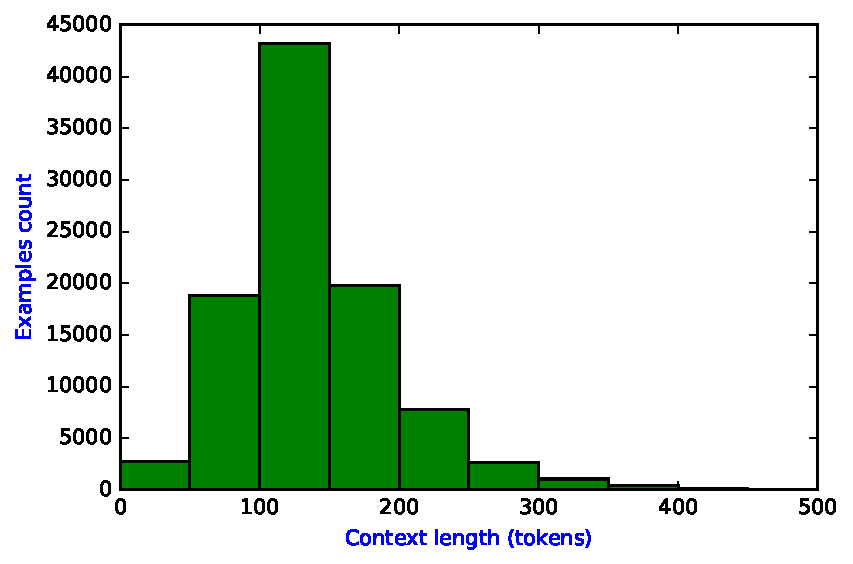
\includegraphics[width=0.3\textwidth]{context}
    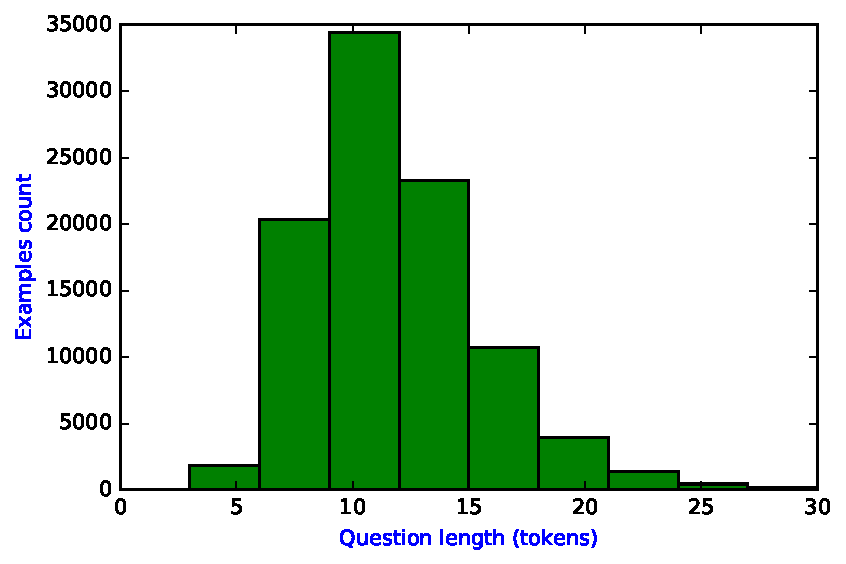
\includegraphics[width=0.3\textwidth]{question}
    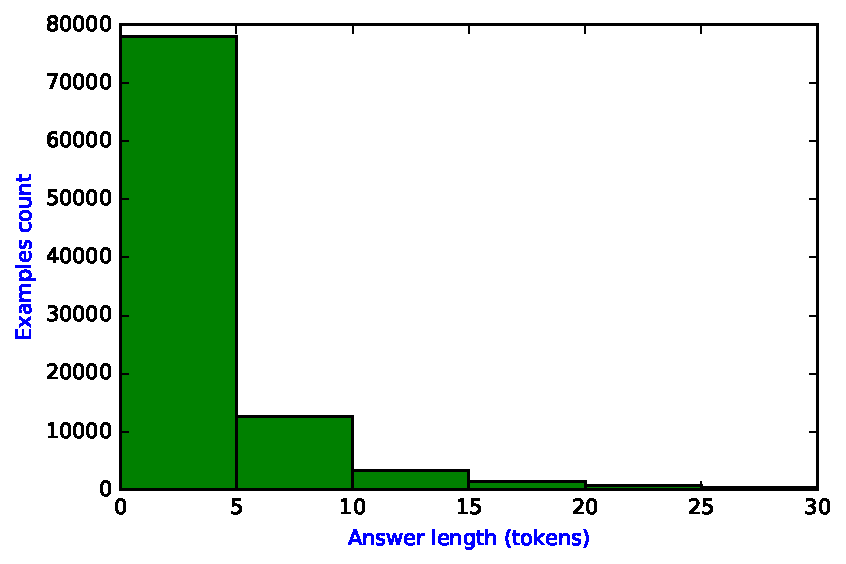
\includegraphics[width=0.3\textwidth]{answer}
    \captionsetup{format=plain, font=footnotesize, labelfont=bf}
    \caption{Data distribution.}
\end{wrapfigure}

2.5 hours for the baseline training still felt like too much, so I decided to reduce my training time further. To achieve it, I sampled ~10 times smaller data set from the training data and did most of my experiments and hyper parameter tuning on it. For example, training baseline to the peak on this data was reduced to ~10-15 minutes. Later, when the model became more complex, the training time increased, but mostly stayed under 1 hour.

Another important point in optimizing training speed is to make sure that GPU is always saturated, as the processing time for batches of different sizes is the same, as long as GPU does not crash with OOM. As a consequence, I am always choosing the largest batch size that could fit into GPU memory.

%\clearpage

\subsection{Improving spans predictions}
After making speed of hyper parameters search reasonable and choosing set of hparams on small data set, I have trained the baseline on the full training data. When looking into the output of this model, one problem was painfully obvious. The model was choosing start and end of an answer span based purely on the softmax output, and it was often producing invalid spans, e.g. spans with the end happening before the start. The simplest possible fix is first to choose a start, and then to choose an end from the interval $[start:]$. But we could do better than that! As we already know (see {\bf Figure 2}) the answers are in general very short, so we can limit this interval further to something like $[start: start + 15)$. Finally, instead of choosing start and end separately based on maximum probability of each, we could, as done in [5], choose the span $(i, j)$ such that $i <= j < i + 15$ and probability $p^{start}(i)*p^{end}(j)$ is maximized. This approach produces slightly better results and the resulting number could be interpreted as a {\it confidence score}, which I will use later when building ensemble.

\begin{table}[h!]
\centering
\setlength{\arrayrulewidth}{0.5mm}
\begin{tabular}{|c || c | c | c | c |} 
 \hline
 Model architecture & F1 score (dev) & EM (dev) & F1 score (test) & EM (test) \\
 \hline
 Baseline & 43.37 & 34.19 & n/a & n/a \\ 
 As above $+$ spans improvements & 50.19 & 39.26 & n/a & n/a \\
 As above $+$ LSTM instead of GRU & 52.37 & 41.15 & n/a & n/a \\
 As above $+$ 1 modeling layer & 65.58 & 54.32 & n/a & n/a \\
 As above $+$ 2 modeling layers & 74.7 & 64.05 & n/a & n/a \\
 As above $+$ bidirectional attention & 74.84 & 64.26 & n/a & n/a \\
 As above $+$ Common Crawl & 75.75 & 65.71 & n/a & n/a \\
 \hline \hline
 Final model (single) & {\bf 76.37} & {\bf 66.00} & n/a & n/a \\
 Final model (ensemble) & 79.01 & 70.31 & {\bf 80.04} & {\bf 71.97} \\
 \hline
 original BiDAF (single model) & 77.3 & 67.7 & 77.3 & 68.0 \\
 original BiDAF (ensemble) & 80.7 & 72.6 & {\bf 81.1} & {\bf 73.3} \\
 \hline
 Current top F1 ([6]) & n/a & n/a & {\bf 89.28} & 82.48 \\
 Current top EM ([6]) & n/a & n/a & 88.76 & {\bf 82.84} \\
 \hline
 Human Performance ([6]) & n/a & n/a & 91.22 & 82.30 \\
 \hline
\end{tabular}
\captionsetup{format=plain, font=large, labelfont=bf}
\caption{Performance results and comparisons}
\end{table}

\subsection{Main modifications}
After fixing basic span prediction errors, I replaced GRU with LSTM, as was suggested by my further hparam search on the small data set, and decided to add the modeling component. Adding it produced the biggest gains of all the changes and became very hard for me to improve upon. For example, replacing basic attention with bidirectional in this architecture was not producing any measurable gains for some time, until I also switched to Common Crawl embedding with much larger vocabulary (see the corresponding F1/EM numbers in {\bf Table 1}). Adding the modeling layer and 300 dimensional embedding led to large increase in model size, which immediately raised an issue of exceeding GPU RAM limit.

\subsection{Reducing memory usage}
Two things that helped the most with lowering my memory consumption were limiting context size and using maximum for combining hidden states in the encoders output instead of concatenation. Applied together, they have reduced memory footprint of the model by the factor of 4. At the same time, the performance drop from using these optimizations was, from my measurements, below 1\%.

Another problem with memory was the size of the checkpoint on disk, which was sometimes large than 100Mb. I solved it purely by luck. When I switched to CommonCrawl embeddings, I have found out that Tensorflow does not support creating tensors larger than 2Gb and that the solution is to create placeholder and feed the embedding into it during run. After this change, checkpoint size dropped below 20Mb even for models with a lot of parameters. I think that without this optimization it would have been much harder for me, if not impossible, to do ensembling later.

\subsection{Things that did not work}
Some things that were used in the BiDAF paper or in some other high performing SQuAD models, like  R-Net [7], for example, just did not work for me for various reasons. One, notably, was Adadelta optimizer. The problem with it that it converges much slower than Adam, so even if it will eventually find a bit better solution, it was just impractical to use under project's time constraints. Another was using additional RNN encoder when predicting ends. I have left this encoder as part of the architecture (turned off by default), but in my experiments I was not able to notice any improvement from using it.

\subsection{Finalizing hyper parameters}
I have listed all the hyper parameters of my best single model in the {\bf Table 2}. To train this model I've switched back to concatenation and increased context length to 400 to improve final performance by additional 1\%. Also, notice that I am not listing batch size in the table. This is because, as I mentioned before, I'm always choosing batch size so that GPU is saturated.

\begin{table}[h!]
\centering
\setlength{\arrayrulewidth}{0.5mm}
\begin{tabular}{|c || c | c |} 
 \hline
 Hyper Parameter & Value & Search Space \\
 \hline
 Optimizer & Adam & \{ Adam; Adadelta \} \\
 Learning rate & 0.003 & \{ 0.1 .. 0.0001 \} \\
 Context length & 400 & \{ 250 .. 600 \} \\
 Context encoder (\# of layers) & 1 &  \{ 1; 2 \} \\
 Context encoder (hidden size) & 100 &  \{ 50 .. 200 \} \\
 Modeling layer (\# of layers) & 2 &  \{ 1; 2; 3 \} \\
 Modeling layer (hidden size) & 75 &  \{ 25 .. 125 \} \\
 Dropout & 0.19 &  \{ 0.1 .. 0.3 \} \\
 RNN cell & LSTM & \{ GRU; LSTM; LayerNormBasicLSTMCell \} \\
 Grad norm & None & \{ None; 1.0 .. 10.0 \} \\
 Combiner & concat & \{ concat; mean; max; average \} \\
 Answer length & 23 & \{ 10 .. 30 \} \\
 \hline
\end{tabular}
\captionsetup{format=plain, font=large, labelfont=bf}
\caption{Final hyper parameters}
\end{table}

\subsection{Ensemble}
To improve the numbers a bit further still I am using ensemble of several most recently trained models. I have tried two techniques for ensembling: choosing an answer of a model with the highest confidence score and "voting", when the answer rating is the sum of confidence scores of the models that have chosen this answer. A bit surprisingly for me, voting performs about two times better than "highest confidence". My expectation before trying was that all the models would likely be choosing a bit different span (because the space to choose from is large) and the situation when the same answer is chosen by more than 1 model will occur very rarely. In reality it seems that the opposite is happening.

To decide whether the specific model should be included into the ensemble, I am using greedy approach. E.g. I am adding models one by one and keep only the ones that improve the results of evaluation. After deciding in this way on a specific set of models to include, I evaluate this ensemble with different limits for answer length set during inference. One surprising thing that I have found from this is that ensembling seems to improve model understanding of longer answers: if for single model optimum limit is around 15, for ensemble it grows with more models added and for 10 models optimum limit rises to 23.

\section{Conclusions}
At the end, I was able to train a high performing model for Reading Comprehension, which achieved competitive ranking on the class leader board. I had several ideas, that I did not have the time to implement, but I still believe that they could improve my model performance further and might be worse trying in the future. One idea was to use some form of a {\bf dynamic padding} instead of limiting context length and, as a result, to avoid even minimal loss of training data. Another was adding self-attention layer from R-Net paper [7] after the bidirectional attention layer. Judging from the official leader board [6], this is a popular and high performing combination. Finally, I think that the span prediction could still be improved further, so it could be interesting to try pointer networks in the future, like done in [8].

{\it The implementation will be made available at \url{github.com/raksitov/squad}.}

\section*{References}

[1] Rajpurkar, P., Zhang, J., Lopyrev, K. and Liang, P., 2016. {\bf Squad: 100,000+ questions for machine comprehension of text.} {\it arXiv preprint arXiv:1606.05250.}

[2] Seo, M., Kembhavi, A., Farhadi, A. and Hajishirzi, H., 2016. {\bf Bidirectional attention flow for machine comprehension.} {\it arXiv preprint arXiv:1611.01603.}

[3] Pennington, J., Socher, R. and Manning, C., 2014. {\bf Glove: Global vectors for word representation.} {\it In Proceedings of the 2014 conference on empirical methods in natural language processing (EMNLP) (pp. 1532-1543).}

[4] Semeniuta, S., Severyn, A. and Barth, E., 2016. {\bf Recurrent dropout without memory loss.} {\it arXiv preprint arXiv:1603.05118.}

[5] Chen, D., Fisch, A., Weston, J. and Bordes, A., 2017. {\bf Reading wikipedia to answer open-domain questions.} {\it arXiv preprint arXiv:1704.00051.}

[6] \url{rajpurkar.github.io/SQuAD-explorer/}

[7] \url{ www.microsoft.com/en-us/research/wp-content/uploads/2017/05/r-net.pdf }

[8] Shuohang Wang and Jing Jiang. {\bf Machine comprehension using match-lstm and answer pointer.}
{\it arXiv preprint arXiv:1608.07905, 2016.}

\end{document}